\newcommand{\institut}{Institut f\"ur Energie und  Automatisiertungstechnik}
\newcommand{\fachgebiet}{Elektronische Mess- und Diagnosetechnik}
\newcommand{\veranstaltung}{Praktikum Messdatenverarbeitung}
\newcommand{\pdfautor}{\"Ozg\"u Dogan (326 048), Timo Lausen (325 411), Boris Henckell (325 779)}
\newcommand{\autor}{\"Ozg\"u Dogan (326 048)\\ Timo Lausen (325 411)\\ Boris Henckell (325 779)}
\newcommand{\pdftitle}{Praktikum Messdatenverarbeitung  Termin 3 und 4}
\newcommand{\prototitle}{Praktikum Messdatenverarbeitung \\ Termin 3 und 4}
\newcommand{\aufgabe}{}

\newcommand{\gruppe}{Gruppe: G1 Fr 08-10}
\newcommand{\betreuer}{Betreuer: J\"urgen Funk}

\input{../../packages/tu_header_8}
%\begin{document}

% \lstlistoflistings
\definecolor{darkgray}{rgb}{0.95,0.95,0.95}
\definecolor{darkolivegreen}{HTML}{01a801}
\definecolor{functionsBlue}{HTML}{32b9b9}
\definecolor{variableRed}{rgb}{1,0,0}
\definecolor{stringBrown}{HTML}{bc8e8e} % f geht nicht

\lstset{
        %\lstset{extendedchars=true} % Umlaute an der richtigen stelle und nicht am Anfang ausgeben
        %basicstyle=\footnotesize\ttfamily,
        basicstyle=\small,
        %
        inputencoding=utf8,
        %
        tabsize=4,
        showspaces=false,
        showtabs=false,
        showstringspaces=true, % no special string spaces
        %
        backgroundcolor=\color{darkgray}, % background
        stringstyle=\color{stringBrown}\fseries, % Strings
        keywordstyle=\color{functionsBlue}\bfseries, % keywords Blau
        identifierstyle=\color{variableRed}, % variablen
        commentstyle=\color{darkolivegreen}, %  comments
        %
        breaklines=true,
        %
        numbers=left,
        numberstyle=\tiny,
        stepnumber=1,
        numbersep=7pt,
        %
        frame=single,
        columns=flexible,
        %
        xleftmargin=-2cm,
        xrightmargin=-1.5cm,
        %
        language=Matlab
}


%---------------------------------------------------------------------
%---------------------------------------------------------------------
%---------------------------------------------------------------------


\section{Vorbereitungsaufgaben}
\begin{quote}
    \subsection{Vorbereitungsaufgaben Termin 3}
    \begin{quote}
        \subsubsection{Sinusfunktion erzeugen und DFT erstellen}
        \begin{quote}
            Die erste Vorbereitungsaufgabe hatte das Ziel einen verschobenes Sinussignal zu erzeugen, die DFT davon zu
            bestimmen und dieses zu plotten. Der dazugehärige Quelltext sinus2.m
            befindet sich im Anhang.
            \begin{figure}[H]
            \centering
                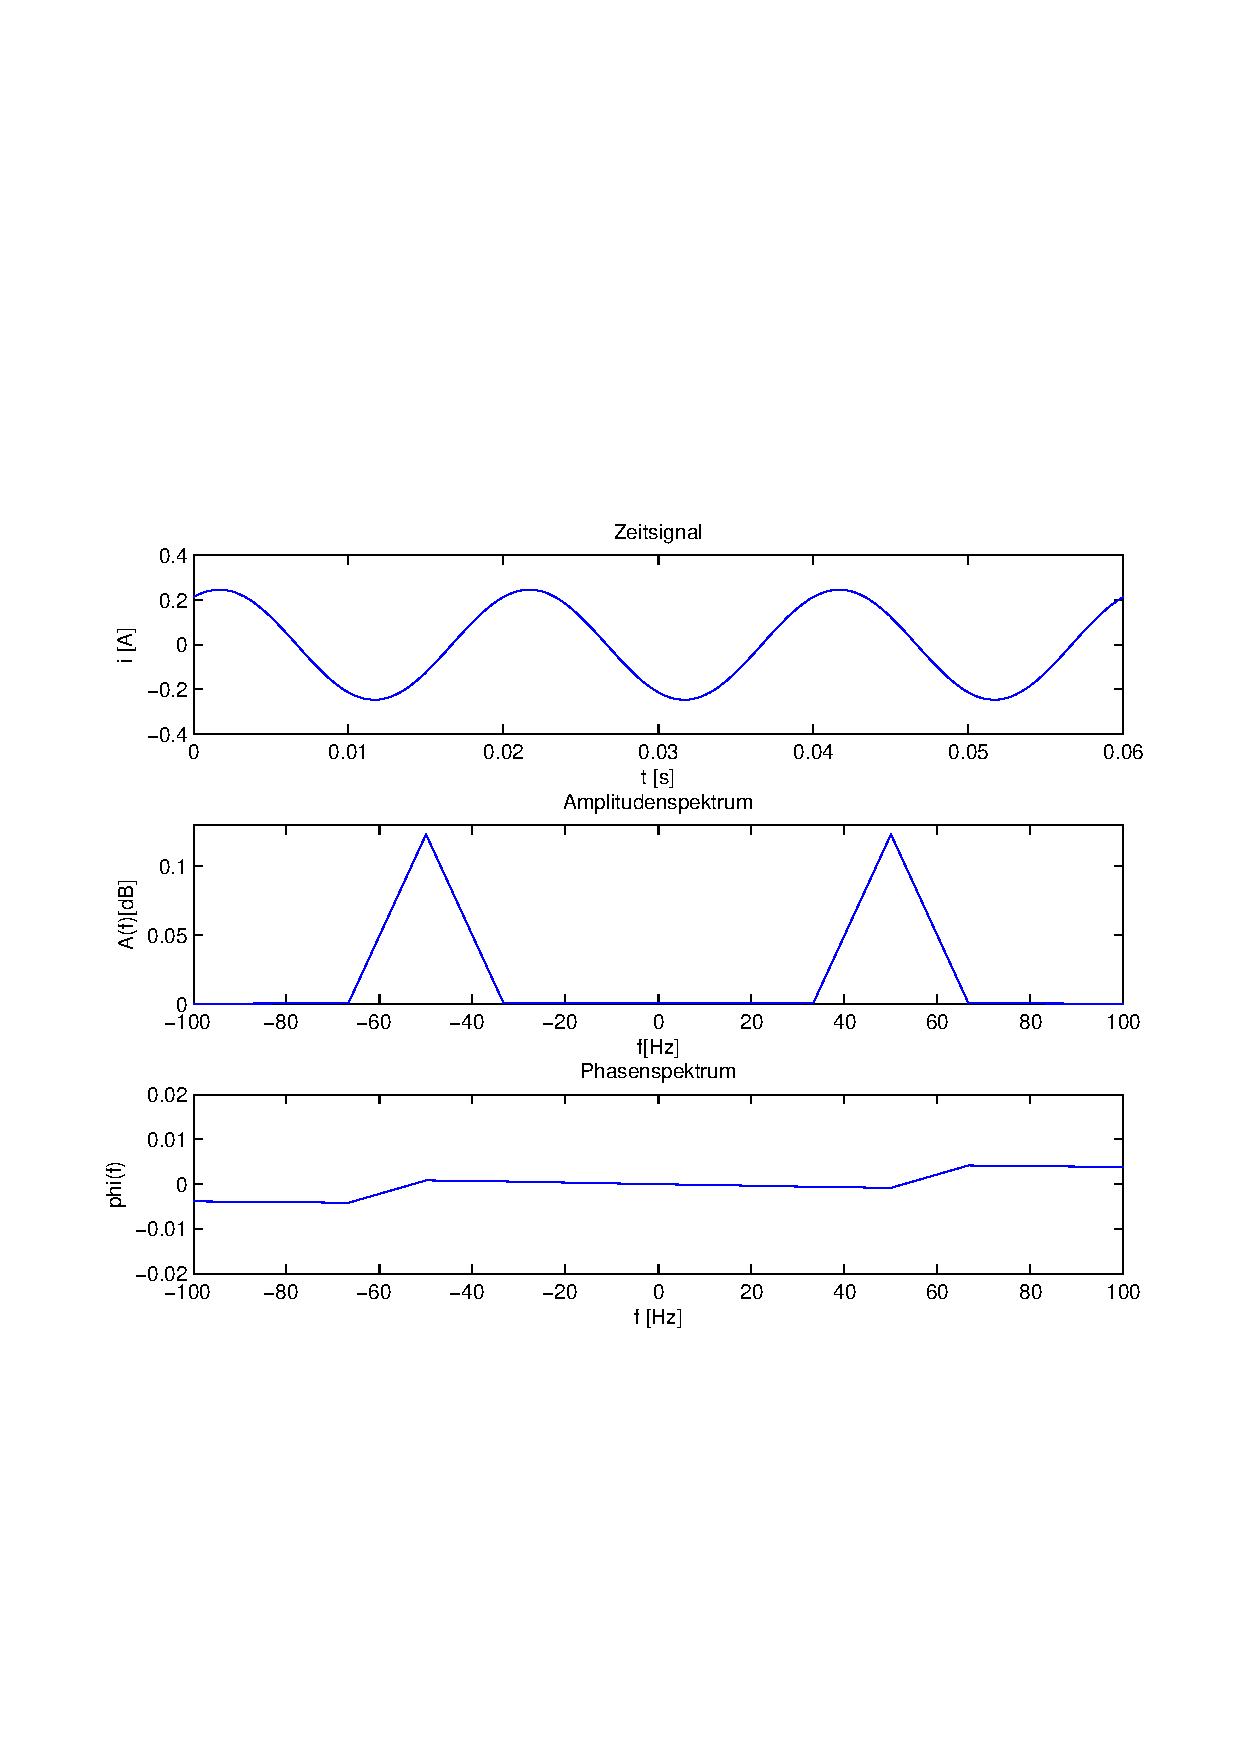
\includegraphics[scale=0.5, trim = 1cm 6cm 1.5cm 8cm, clip]{./Bilder/VerschobenerSinusAufgabe1}
                    \caption{Verschobener Sinus}
                    \label{fig:./Bilder/VerschobenerSinusAufgabe1}
            \end{figure}
        
        \end{quote}
        
    	\subsubsection{Angeschnittene Sinusfunktion}
        \begin{quote}
            In der zweiten Vorbereitungsaufgabe sollte eine Matlab-Funktion
            geschrieben werden, die einen angeschnittene Sinusfunktion simuliuliert.\\
            Um diese Funktion zu erstellen haben wir eine for Schleife
            imlementiert, die den gesamten Zeitvektor t durchläuft. Für jeden Durchlauf wird getestet, 
            wo sich der jeweilige Zeitpunkt im Verhältniss zum halben
            Sinussignal befindet. Anschließend wird in der if Abfrage bestimmt, ob sich dieser Zeitpunkt relativ zur halben
            Periode des Sinussignals vor oder hinter dem Phasenanschnittswinkel befindet. Abhängig davon wird der
            dementsprechenden Stelle im Ausgabevektor der Wert $0$ oder der
            Wert, den die Sinusfunktion ermittelt, übergeben.\\
            Wir haben die Graphen für folgende Phasenanschnittswinkel $ \alpha = 0, \frac{1}{8} \pi, \frac{1}{4}
            \pi, \frac{3}{8} \pi, \frac{1}{2} \pi,\frac{5}{8} \pi, \frac{3}{4} \pi, \frac{7}{8} \pi$ und $\pi$
            geplottet.\\
            Der dazugehärige Quelltext befindet sich im Anhang.
        \end{quote}
        
        \subsubsection{Effektivwert des Stroms im Zeitbereich}
        \begin{quote}
            Für den Effektivwert des Stroms im Zeitbereich ermitteln wir die Wurzel des Mittelwertes des Quadrats des
            Stromvektors.\\
            Der dazugehörige Quelltext befindet sich im Anhang.
        \end{quote}
        
        \subsubsection{Effektivwert des Stroms im Frequenzbereich}
        \begin{quote}
            Den Effektivwert des Stroms im Frequenzbereich ermitteln wir ähnlich wie den Effektivwert des Stroms im
            Zeitbereich. Das Parsevalschen-Theorem besagt, dass die Energien eines Signals im Zeitbereich gleich seiner
            Energie im Frequenzbereich ist.\cite{PasevalscheTheorem}\\
            \begin{equation*}
            	\begin{split}
            		\sum_{n=0}^{N-1} |x[n]|^2 = \frac{1}{N} \sum_{k=0}^{N-1} |X[k]|^2
            	\end{split}
            \end{equation*}
            
            Der dazugehörige Quelltext befindet sich im Anhang.
            \end{quote}
        \subsubsection{Ergebnisse Vorbereitungsaufgaben}
        \begin{quote}
                                    %4 Grafiken:
                \begin{center}
                \begin{tabular}{ll}
    
                \hspace{-11em}
                    \begin{minipage}{0.6\textwidth}
    
                        \begin{figure}[H]
                            \label{fig:}
                            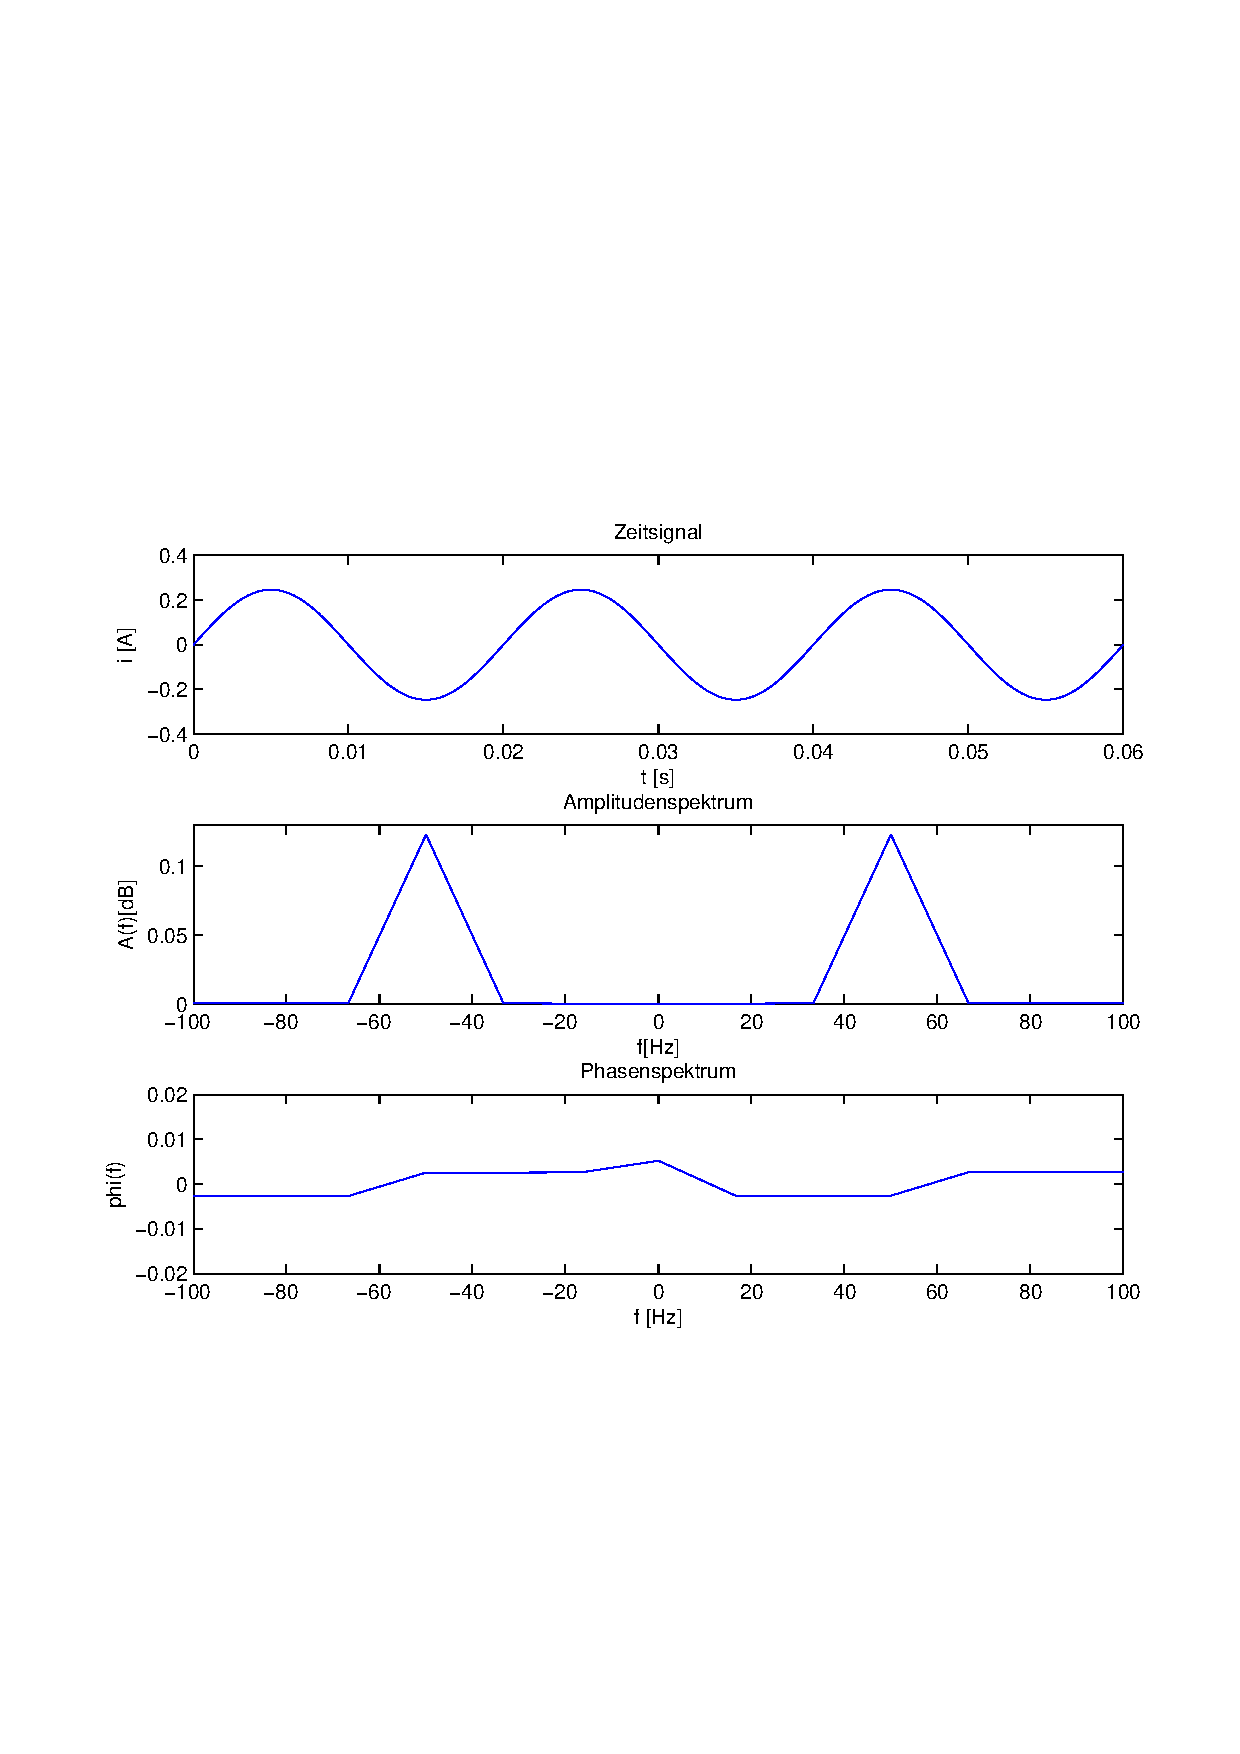
\includegraphics[scale=0.5, trim = 1.5cm 7cm 1.5cm 8.5cm,
                            clip]{./Bilder/Phasenanschnitt08pi.pdf}
                            %FIXME [width=640px,
                             %height=474px]
                            \caption{Sinussignal mit Phasenanschnitt von $0$}
                        \end{figure}
    
                    \end{minipage}
                    \begin{minipage}{0.6\textwidth}
    
                        \begin{figure}[H]
                            \label{fig:}
                            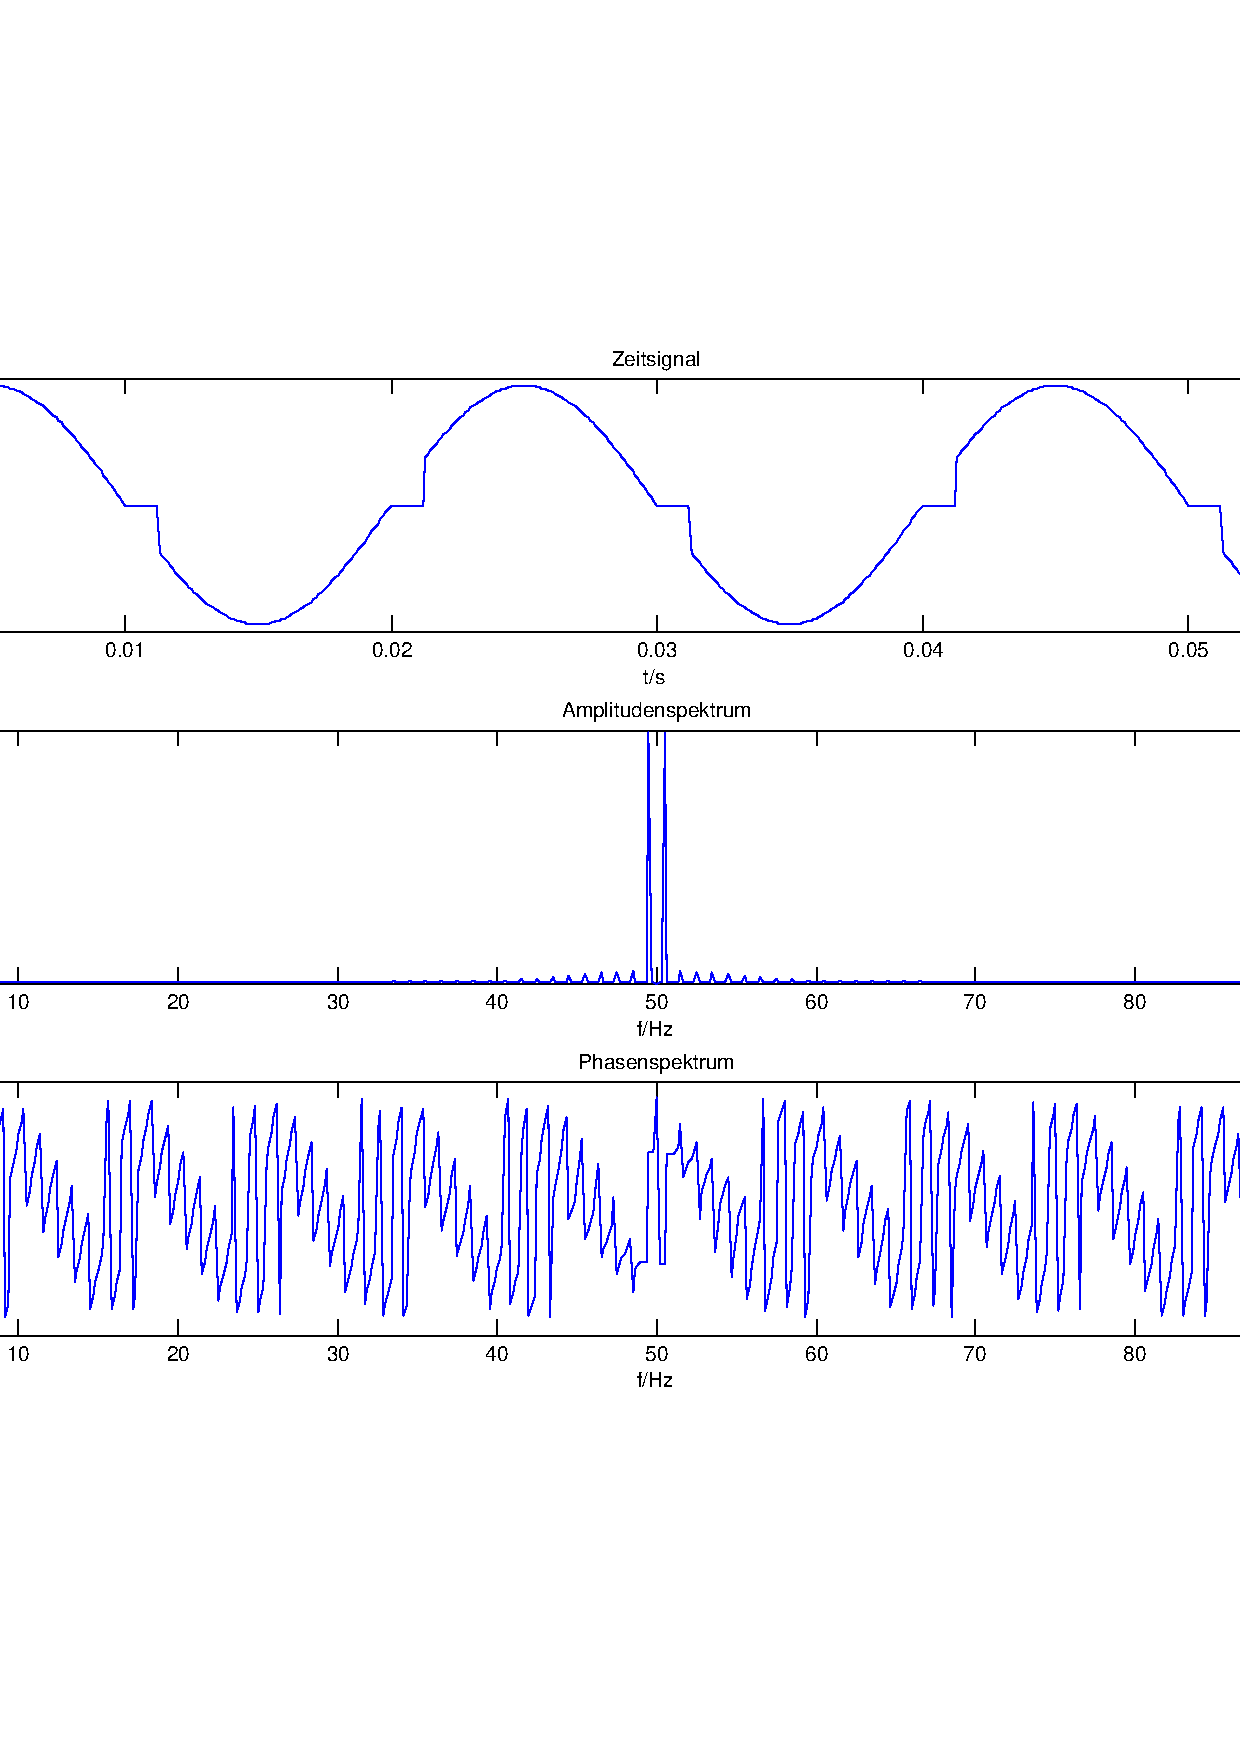
\includegraphics[scale=0.5, trim = 1.5cm 7cm 1.5cm 8.5cm,
                            clip]{./Bilder/Phasenanschnitt18pi.pdf}
                            %FIXME [width=640px,
                             %height=474px]
                            \caption{Sinussignal mit Phasenanschnitt von $\frac{1}{8}/pi$}
                        \end{figure}
                    \vspace{-1.5em}
    
                    \end{minipage}
    
                \end{tabular}
                \end{center}
    
                            %4 Grafiken:
                \begin{center}
                \begin{tabular}{ll}
    
                \hspace{-11em}
                    \begin{minipage}{0.6\textwidth}
    
                        \begin{figure}[H]
                            \label{fig:}
                            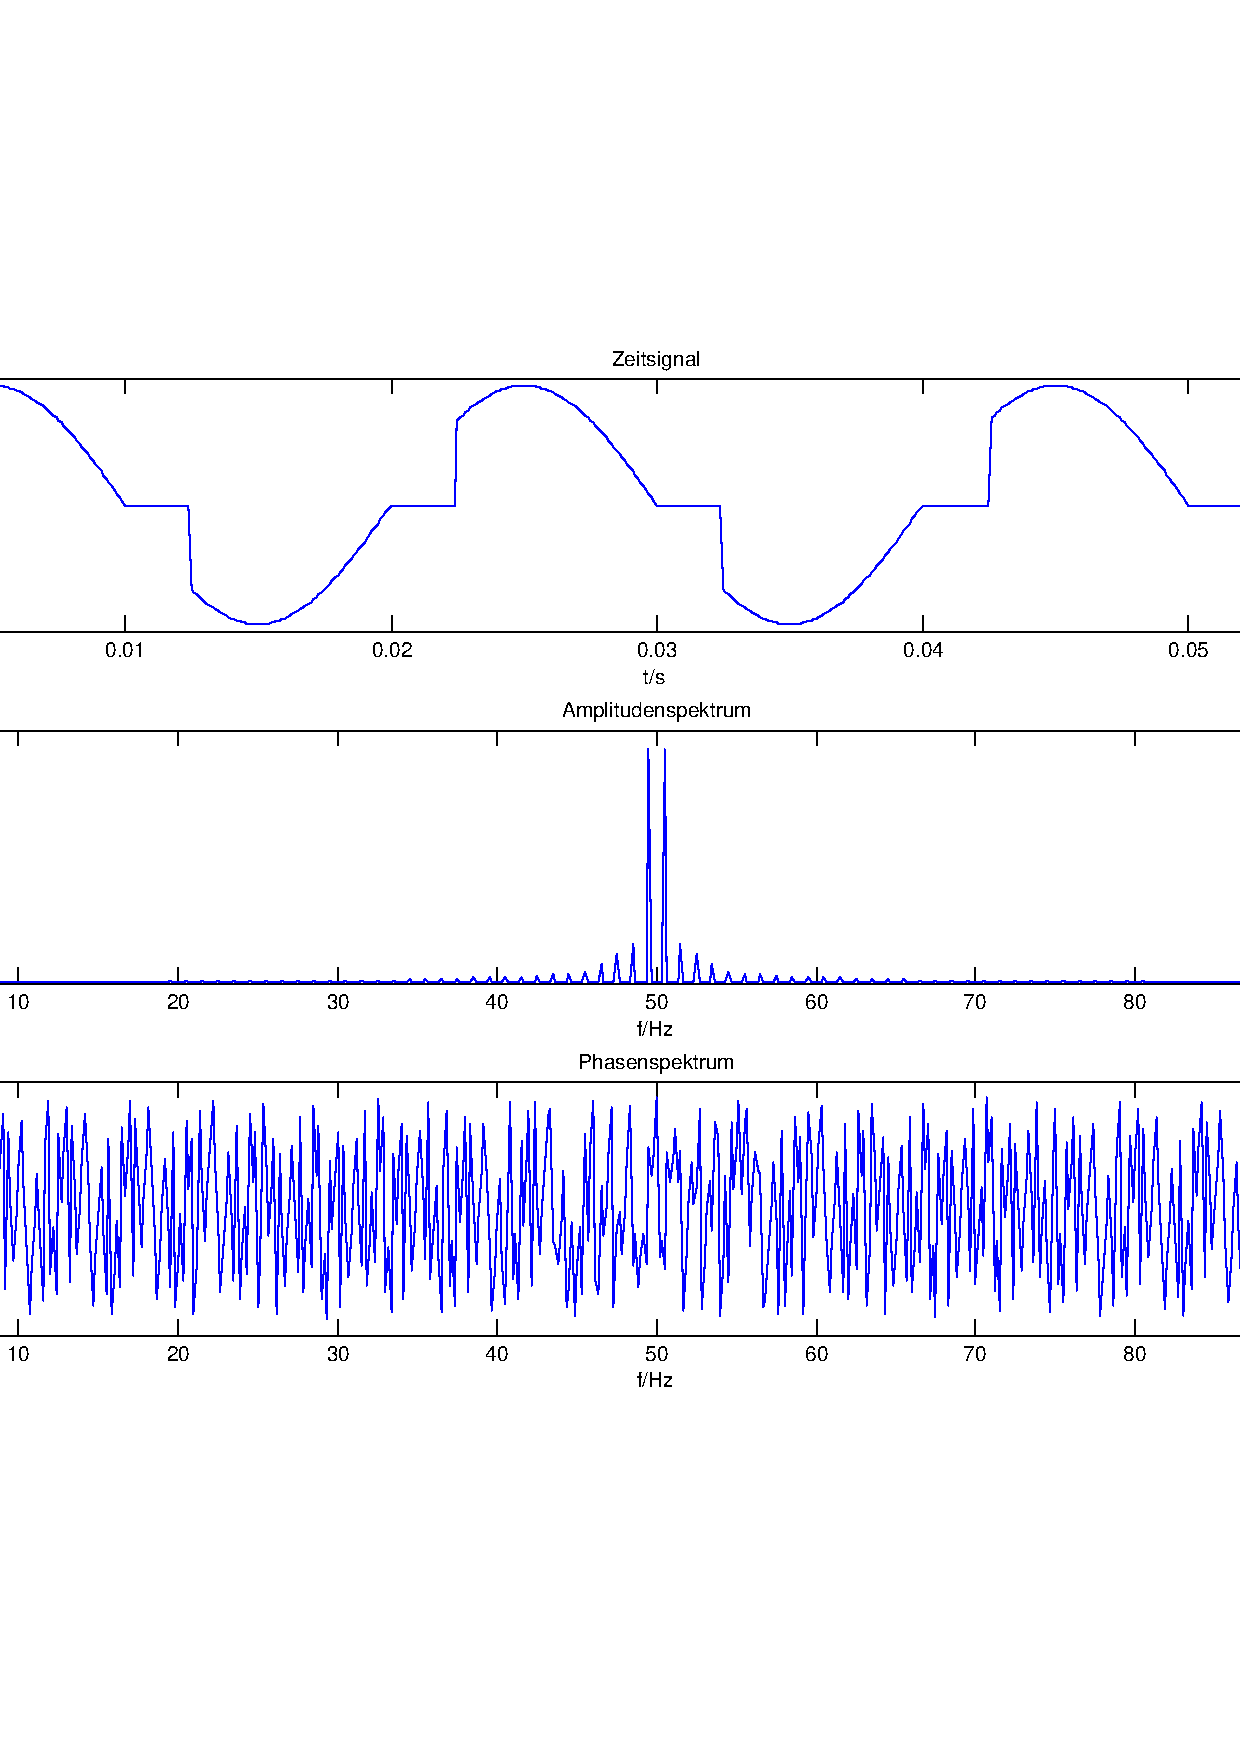
\includegraphics[scale=0.5, trim = 1.5cm 7cm 1.5cm 8.5cm,
                            clip]{./Bilder/Phasenanschnitt28pi.pdf} %FIXME [width=640px, height=474px]
                            \caption{Sinussignal mit Phasenanschnitt von $\frac{1}{4}/pi$}
                        \end{figure}
    
                    \end{minipage}
                    \begin{minipage}{0.6\textwidth}
    
                         \begin{figure}[H]
                            \label{fig:}
                            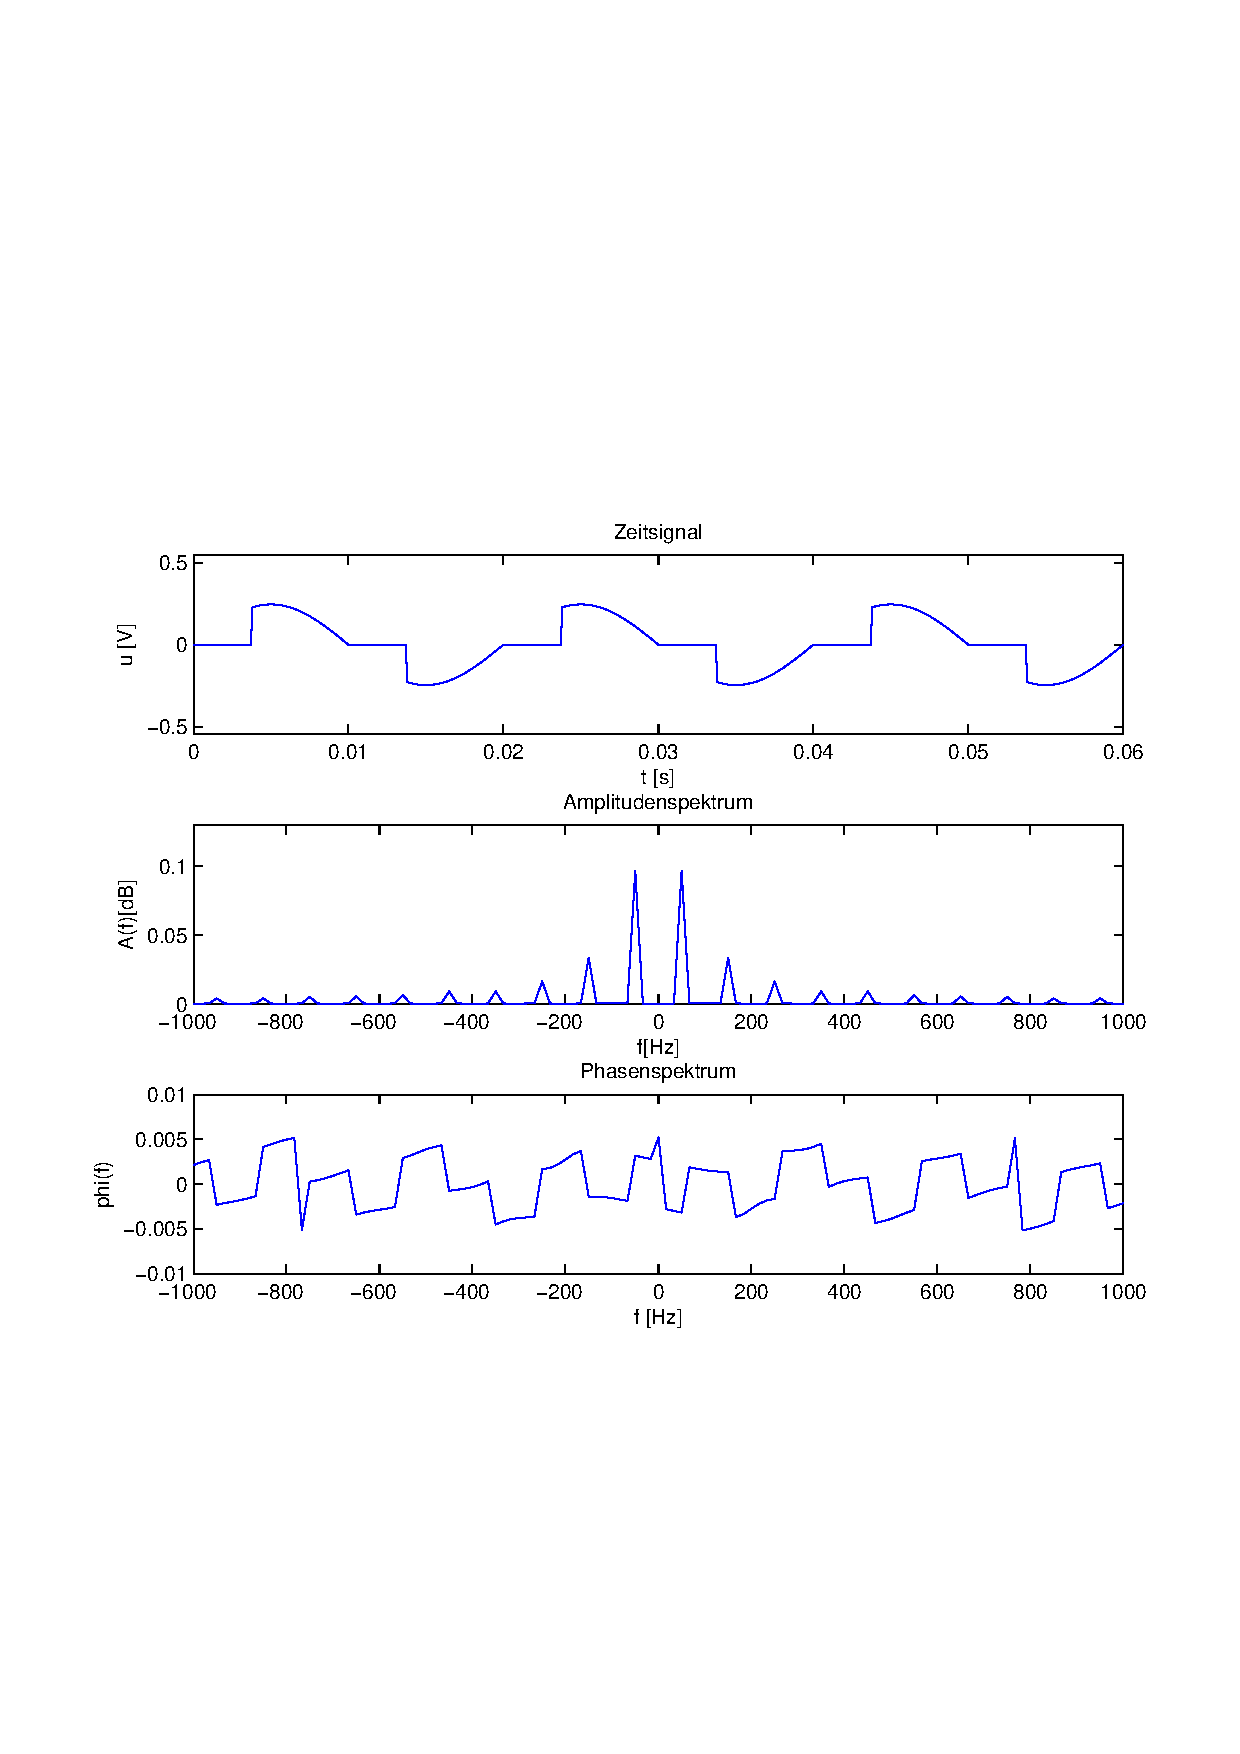
\includegraphics[scale=0.5, trim = 1.5cm 7cm 1.5cm 8.5cm,
                            clip]{./Bilder/Phasenanschnitt38pi.pdf} %FIXME [width=640px, height=474px]
                            \caption{Sinussignal mit Phasenanschnitt von $\frac{3}{8}/pi$}
                        \end{figure}
                   \vspace{-1.5em}
    
                    \end{minipage}
    
                \end{tabular}
                \end{center}
    
                            %4 Grafiken:
                \begin{center}
                \begin{tabular}{ll}
    
                \hspace{-11em}
                    \begin{minipage}{0.6\textwidth}
    
                        \begin{figure}[H]
                            \label{fig:}
                            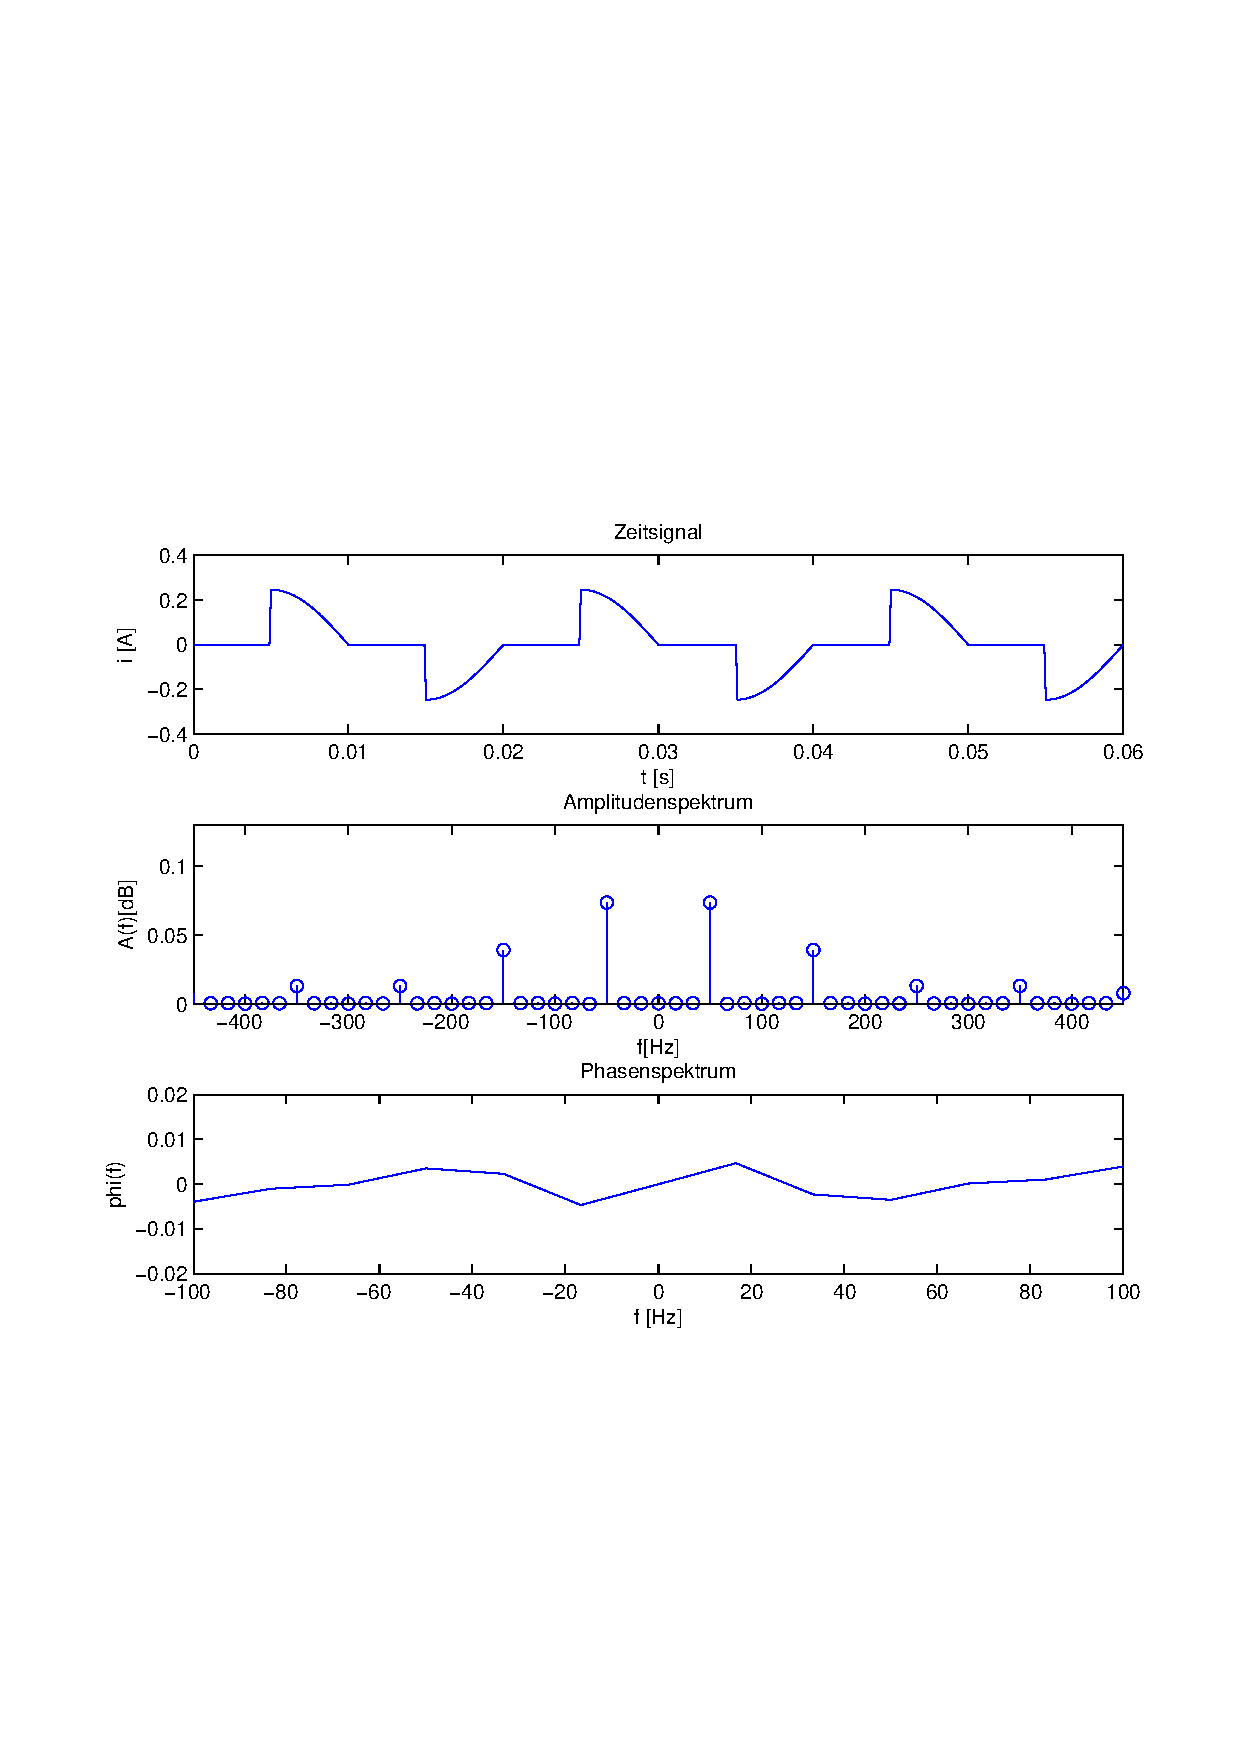
\includegraphics[scale=0.5, trim = 1.5cm 7cm 1.5cm 8.5cm,
                            clip]{./Bilder/Phasenanschnitt48pi.pdf} %FIXME [width=640px, height=474px]
                            \caption{Sinussignal mit Phasenanschnitt von $\frac{1}{2}/pi$}
                        \end{figure}
    
                    \end{minipage}
                    \begin{minipage}{0.6\textwidth}
    
                       \begin{figure}[H]
                            \label{fig:}
                            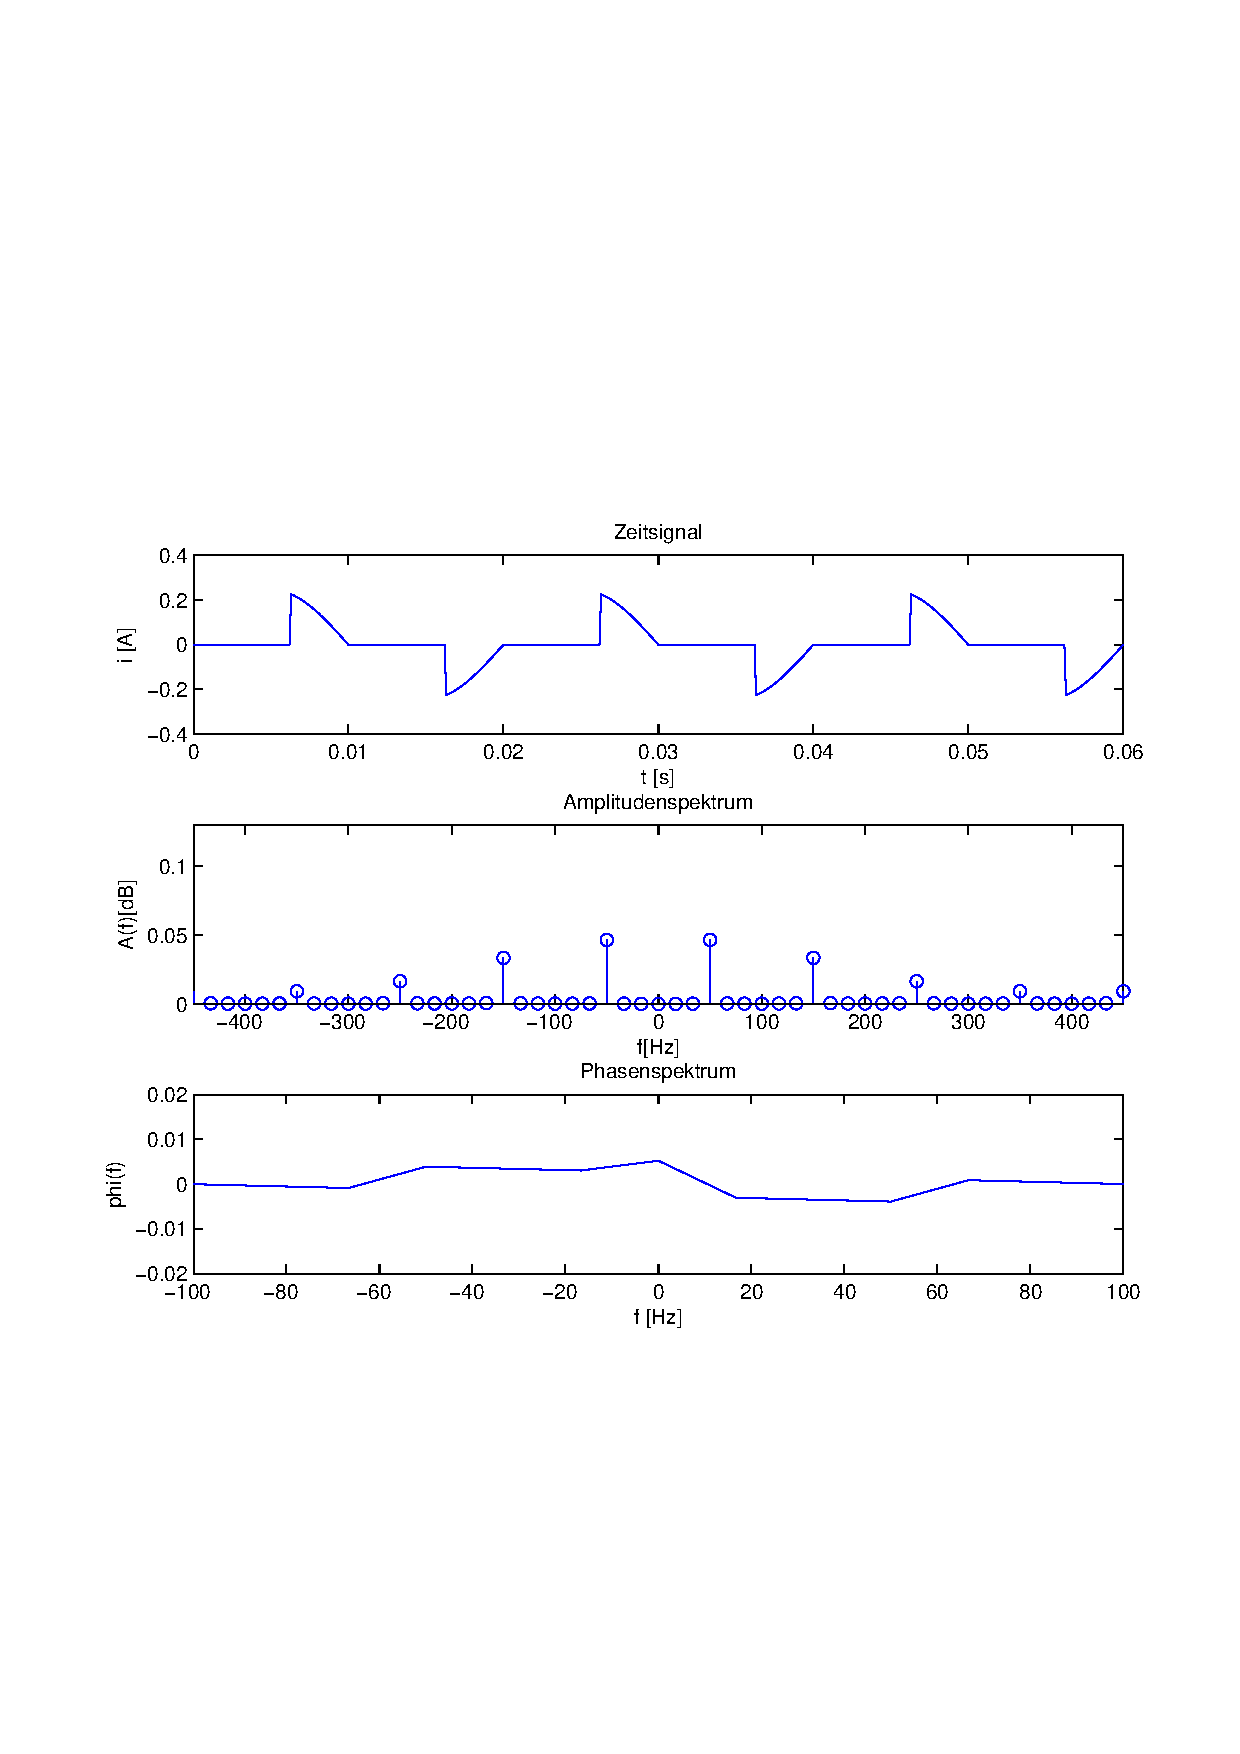
\includegraphics[scale=0.5, trim = 1.5cm 7cm 1.5cm 8.5cm,
                            clip]{./Bilder/Phasenanschnitt58pi.pdf} %FIXME [width=640px, height=474px]
                            \caption{Sinussignal mit Phasenanschnitt von $\frac{5}{8}/pi$}
                        \end{figure}
                     \vspace{-1.5em}
    
                    \end{minipage}
    
                \end{tabular}
                \end{center}
    
                   %4 Grafiken:
                \begin{center}
                \begin{tabular}{ll}
    
                \hspace{-11em}
                    \begin{minipage}{0.6\textwidth}
    
                        \begin{figure}[H]
                            \label{fig:}
                            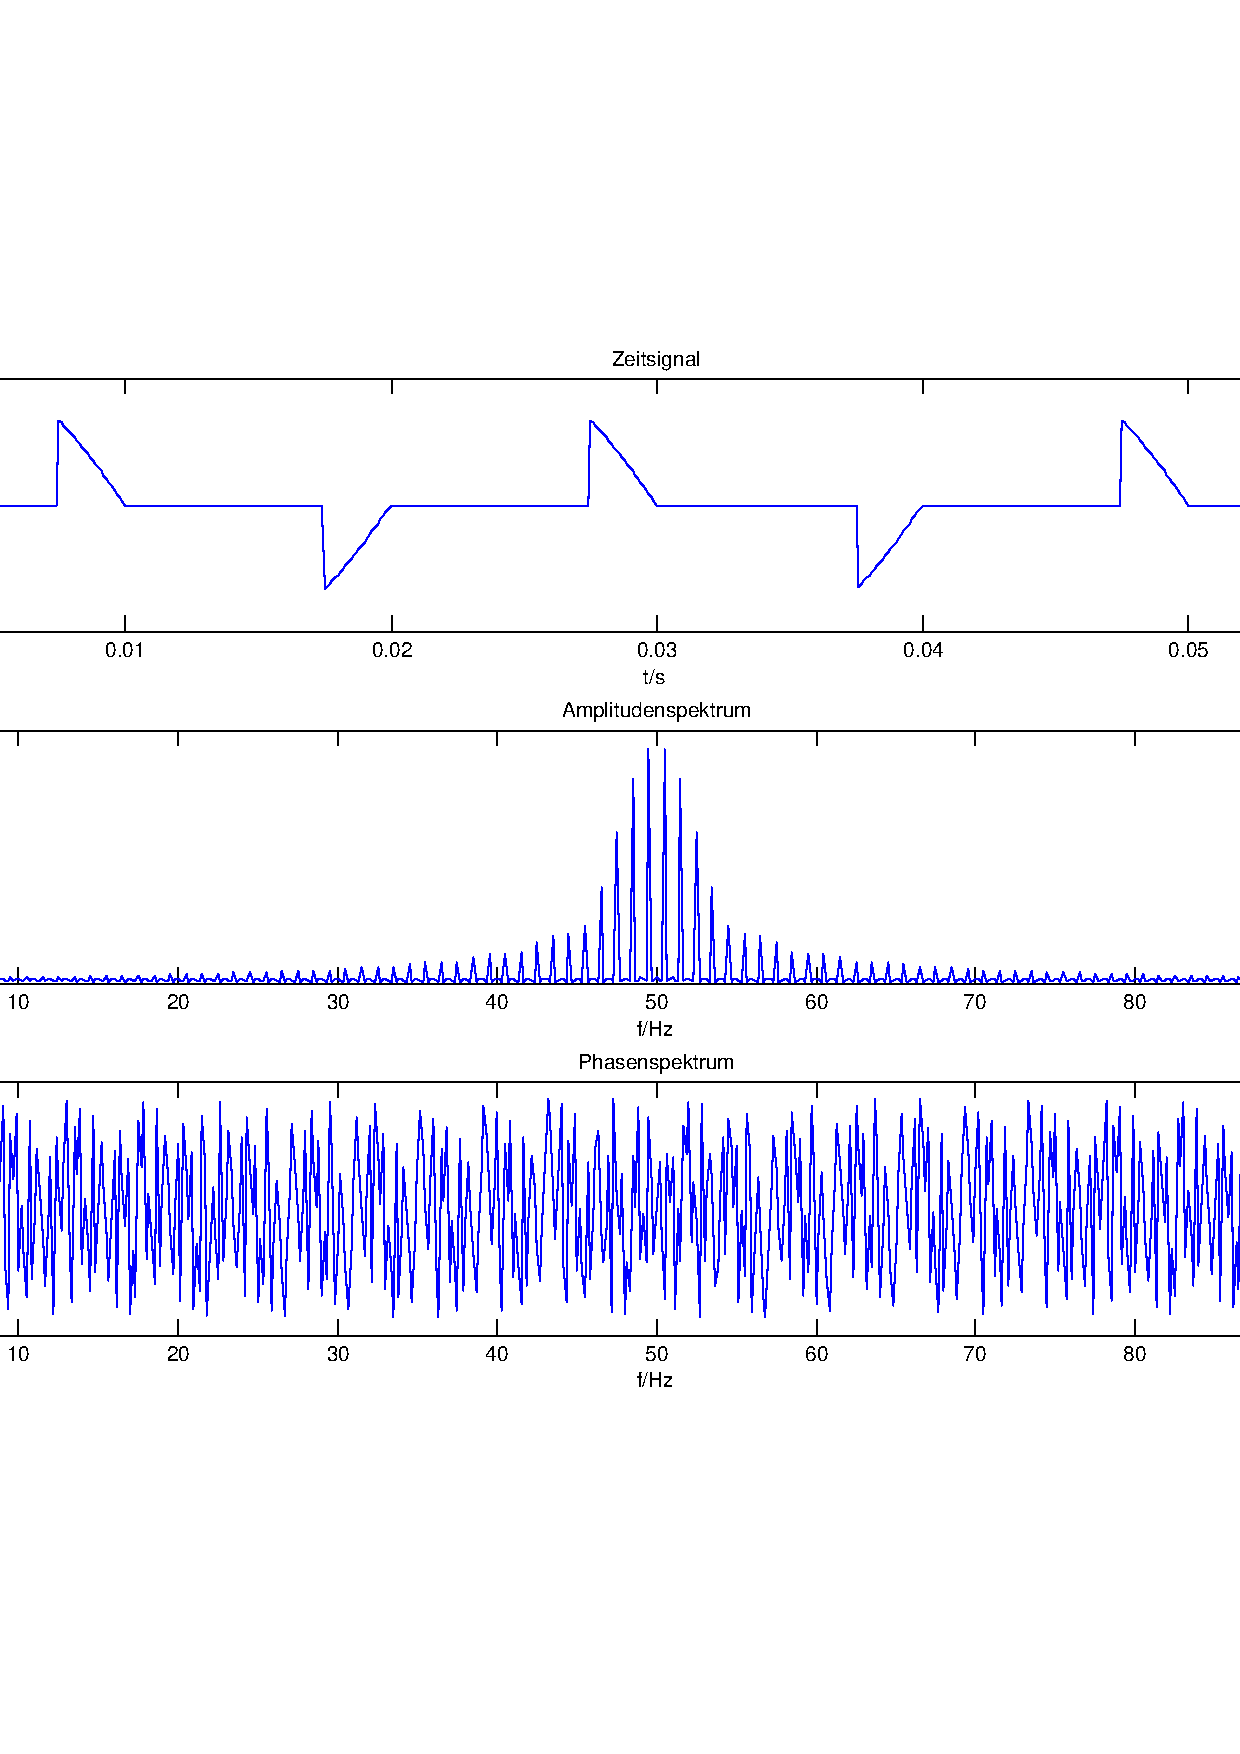
\includegraphics[scale=0.5, trim = 1.5cm 7cm 1.5cm 8.5cm,
                            clip]{./Bilder/Phasenanschnitt68pi.pdf} %FIXME [width=640px, height=474px]
                            \caption{Sinussignal mit Phasenanschnitt von $\frac{3}{4}/pi$}
                        \end{figure}
    
                    \end{minipage}
                    \begin{minipage}{0.6\textwidth}
    
                       \begin{figure}[H]
                            \label{fig:}
                            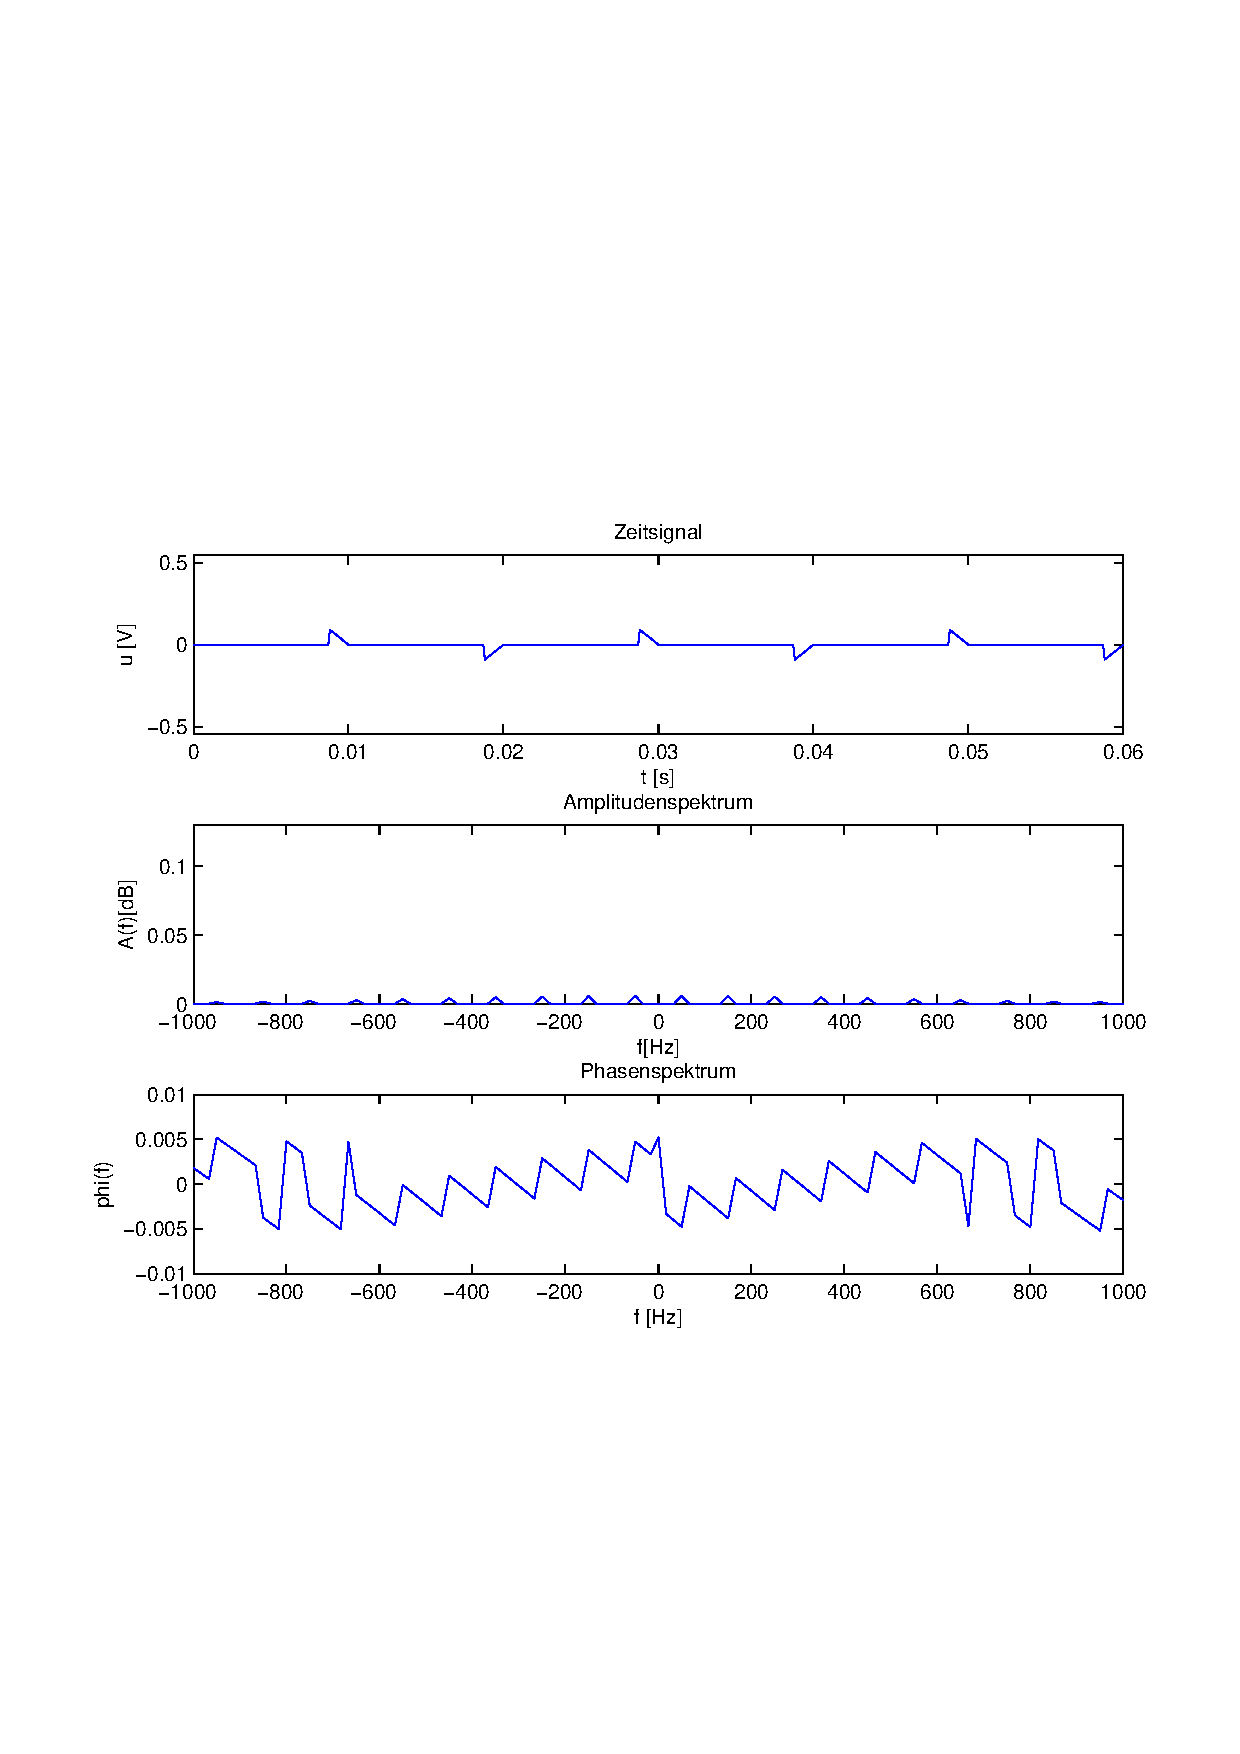
\includegraphics[scale=0.5, trim = 1.5cm 7cm 1.5cm 8.5cm,
                            clip]{./Bilder/Phasenanschnitt78pi.pdf} %FIXME [width=640px, height=474px]
                            \caption{Sinussignal mit Phasenanschnitt von $\frac{7}{8}/pi$}
                        \end{figure}
                     \vspace{-1.5em}
    
                    \end{minipage}
    
                \end{tabular}
                \end{center}
                
                   %4 Grafiken:
                \begin{center}
                \begin{tabular}{ll}
    
                \hspace{-4em}
                    \begin{minipage}{0.6\textwidth}
    
                        \begin{figure}[H]
                            \label{fig:}
                            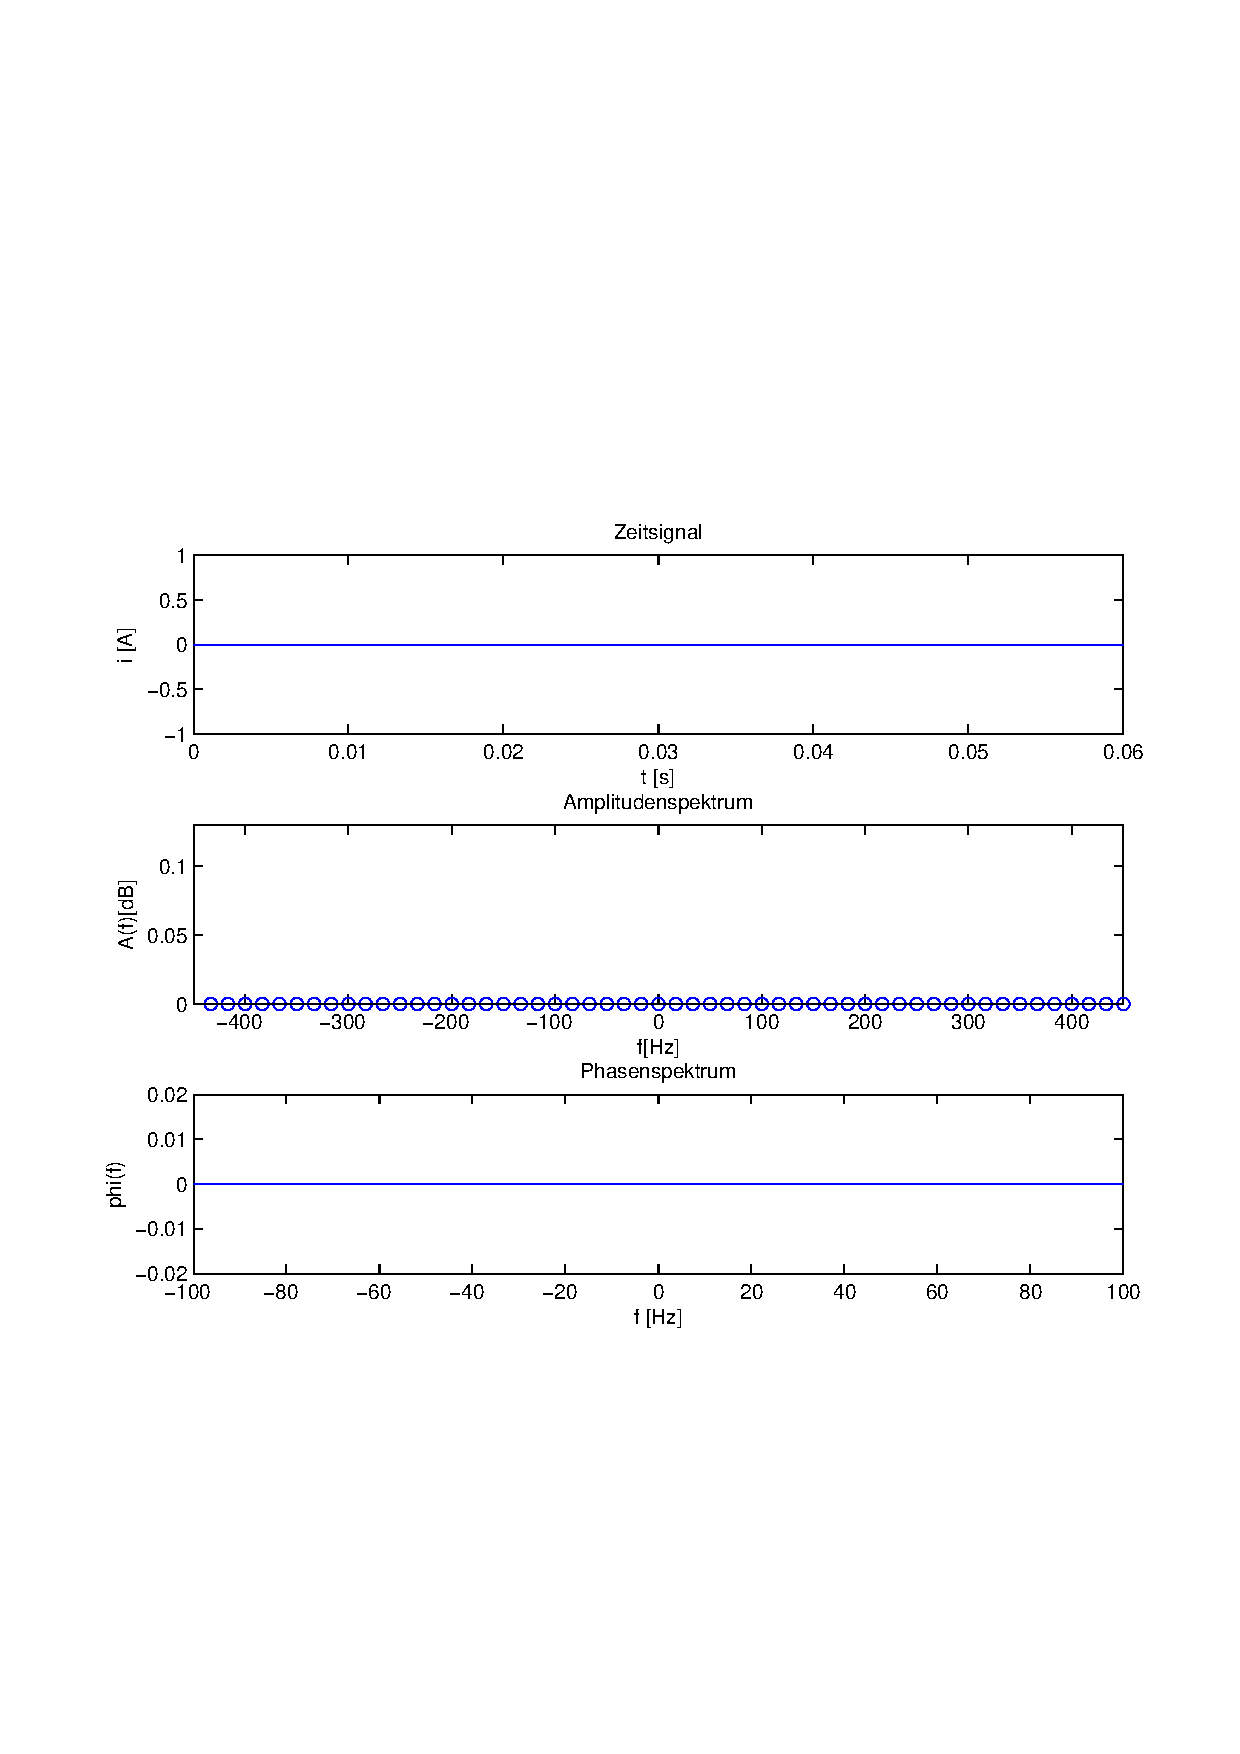
\includegraphics[scale=0.5, trim = 1.5cm 7cm 1.5cm 8.5cm,
                            clip]{./Bilder/Phasenanschnitt88pi.pdf} %FIXME [width=640px, height=474px]
                            \caption{Sinussignal mit Phasenanschnitt von $/pi$}
                        \end{figure}
    
                    \end{minipage}
    
                \end{tabular}
                \end{center}
                 \begin{center}
                     \begin{tabular}{|c|c|c|}
                                 
                       \hline
                       $\alpha $ & $i_{eff}$ (Zeitbereich) & $i_{eff}$ Frequenzbereich\\ \hline
                       $0$ & 3,5326 & 3,5326 \\ \hline
                       $\frac{1}{8} \pi$ & 3,5105 & 3,5105 \\ \hline
                       $\frac{1}{4} \pi$ & 3,3744 & 3,3744 \\ \hline
                       $\frac{3}{8} \pi$ & 3,0338 & 3,0338 \\ \hline
                       $\frac{1}{2} \pi$ & 2,5145 & 2,5145 \\ \hline
                       $\frac{5}{8} \pi$ & 1,8097 & 1,8097 \\ \hline
                       $\frac{3}{4} \pi$ & 1,0748 & 1,0748 \\ \hline
                       $\frac{7}{8} \pi$ & 0,3940 & 0,3940 \\ \hline
                       $ \pi$ & 0 & 0 \\ \hline
                             
               
                     \end{tabular}
                 \end{center}        
        \end{quote}
    \end{quote}
    \subsection{Vorbereitungsaufgaben Termin 4}
    \begin{quote}
        In dem zweiten Teil der Vorbereitungsaufgaben ging es um Fensterung. Mit
        unterschiedlichen Fensterfunktionen kann man Analysefenster erschaffen,
        die ein ganzzahliges Vielfaches der Periodendauer des Messsignals lang
        sind. Somit kann man bei der Untersuchung der Signale Leck-Effekte
        verhindern.\\
       
        \subsubsection{Matlabfunktion-Spektrum}
		\begin{quote}
            Dafür machten wir uns mit unterschiedlichen Fensterfunktionen vertraut und schrieben eine MATLAB Funktion,
            mit der ein Fenster generiert werden konnte, dessen Länge genau einer Periodenlänge des verwendeten Signals
            entspricht. Zusätzlich wurden Fenster und Signal überlagert und die DFT gebildet, Betrags- und
            Phasenspektren wurden geplottet.\\
            Das dazugehärige Matlabscripte Spektrum.m sowie Vorbereitungsaufgabe42.m befindet sich im Anhang.\\
            In diesem Skript haben wir ein Sinussignal mit der Frequenz $100$Hz erzeugt und jeweils mit einem Rechteck-,
            einem BlackMan-, einem Hanning- sowie einem verkürztem Hanningfenster multipliziert.\\
            Die Plotts dazu sind hier:
            
                            %4 Grafiken:
                \begin{center}
                \begin{tabular}{ll}
    
                \hspace{-11em}
                    \begin{minipage}{0.6\textwidth}
    
                        \begin{figure}[H]
                            \label{fig:}
                            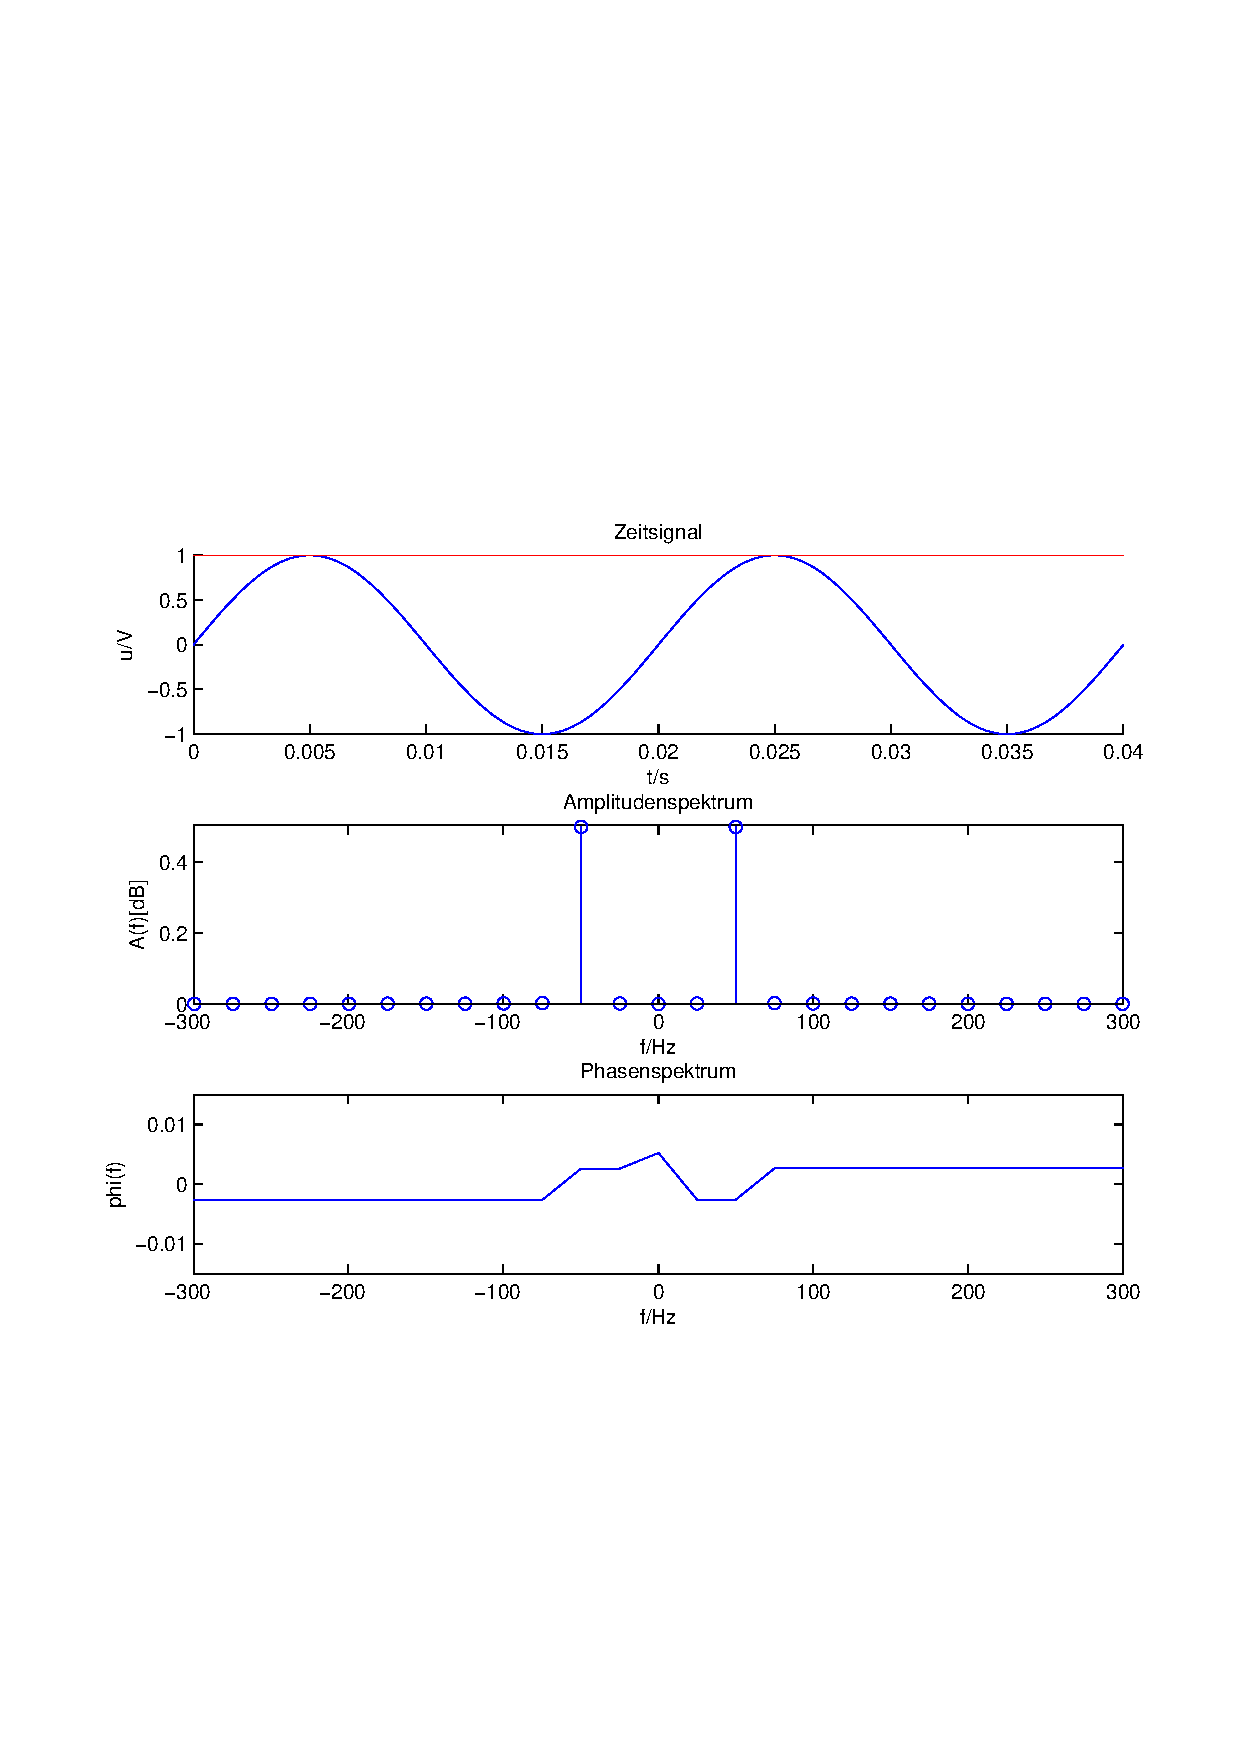
\includegraphics[scale=0.5,trim = 1.5cm 7cm 1.5cm 8cm, clip]{./Bilder/Rechteckwindow}
                            %FIXME [width=640px,
                             %height=474px]
                            \caption{DFT eines Rechteckfensters}
                        \end{figure}
    
                    \end{minipage}
                    \begin{minipage}{0.6\textwidth}
    
                        \begin{figure}[H]
                            \label{fig:}
                            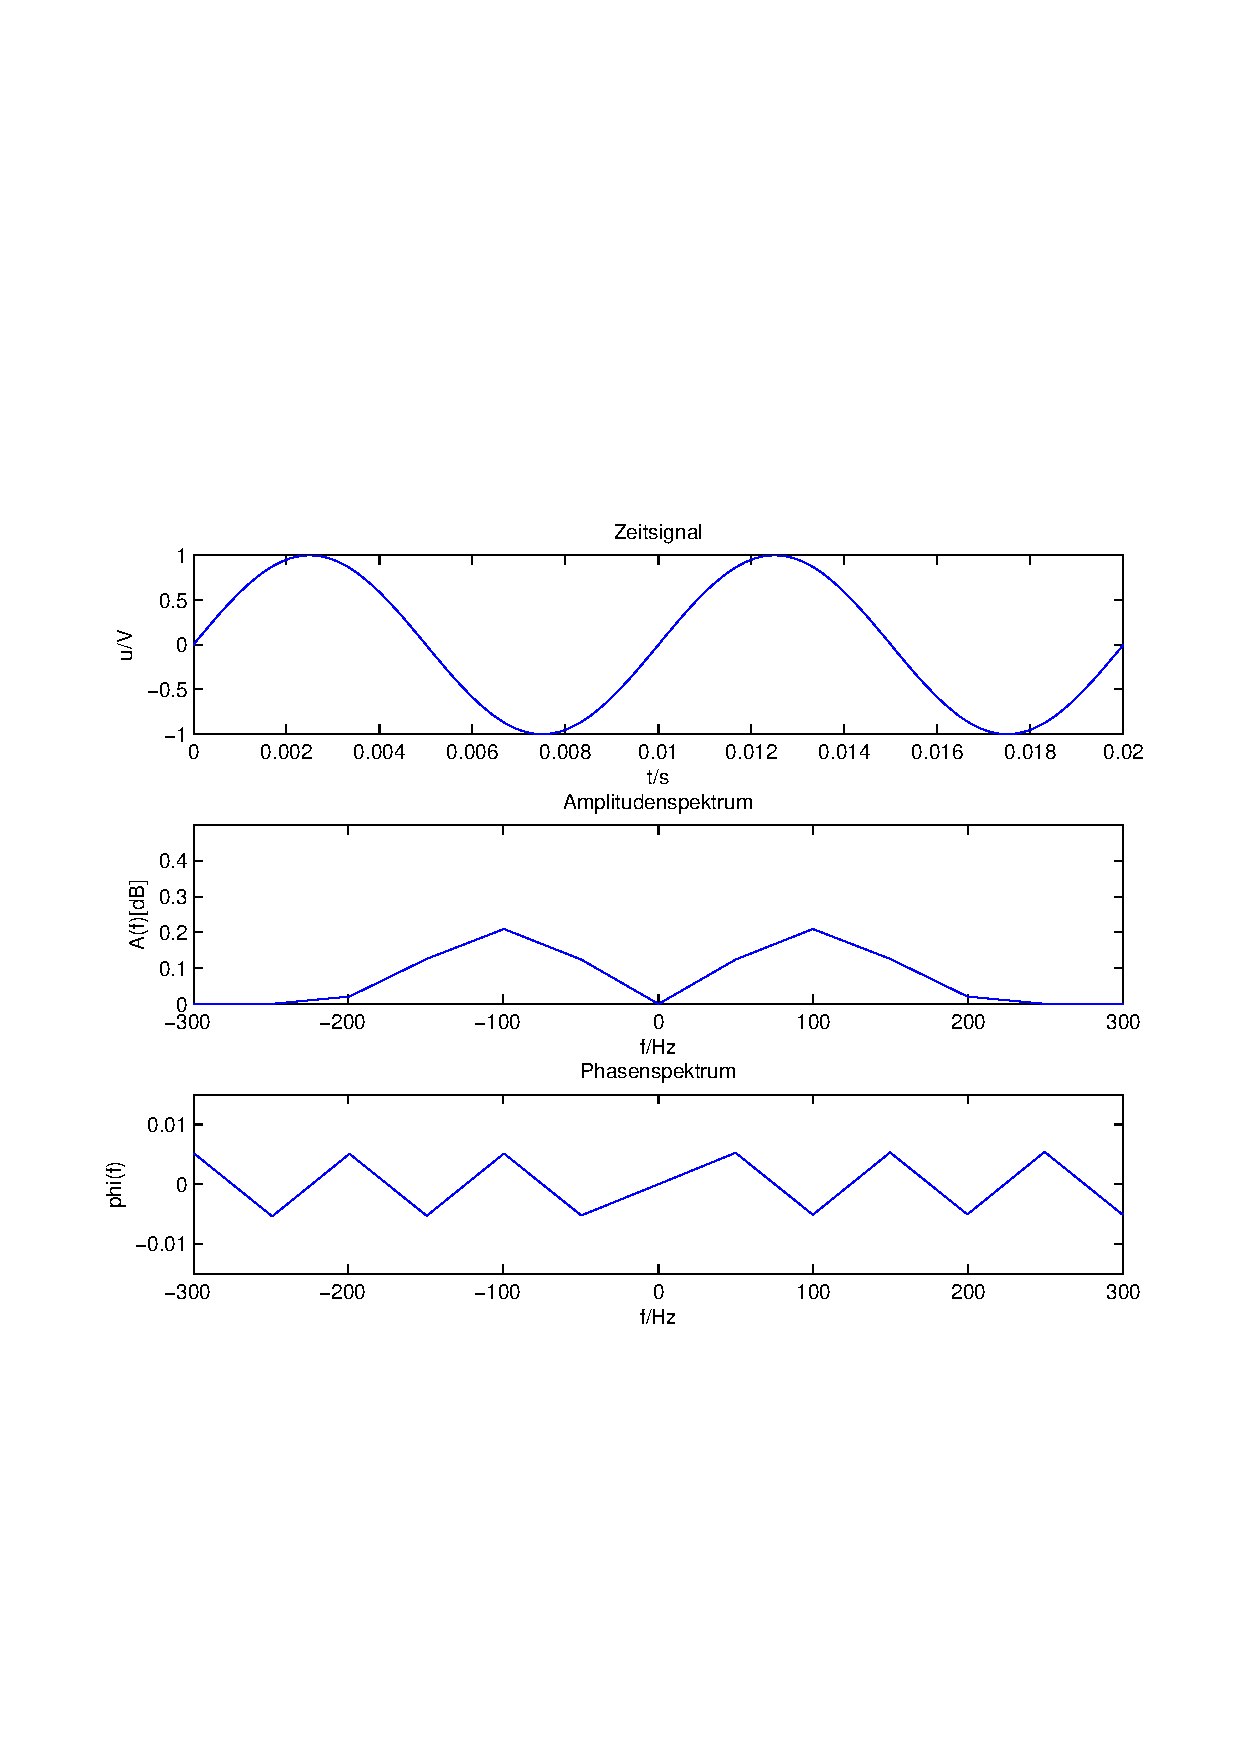
\includegraphics[scale=0.5,trim = 1.5cm 7cm 1.5cm 8cm, clip]{./Bilder/BlackManwindow}
                            %FIXME [width=640px,
                             %height=474px]
                            \caption{DFT eines Hanningfensters}
                        \end{figure}
                    \vspace{-1.5em}
    
                    \end{minipage}
    
                \end{tabular}
                \end{center}
    
                            %4 Grafiken:
                \begin{center}
                \begin{tabular}{ll}
    
                \hspace{-11em}
                    \begin{minipage}{0.6\textwidth}
    
                        \begin{figure}[H]
                            \label{fig:}
                            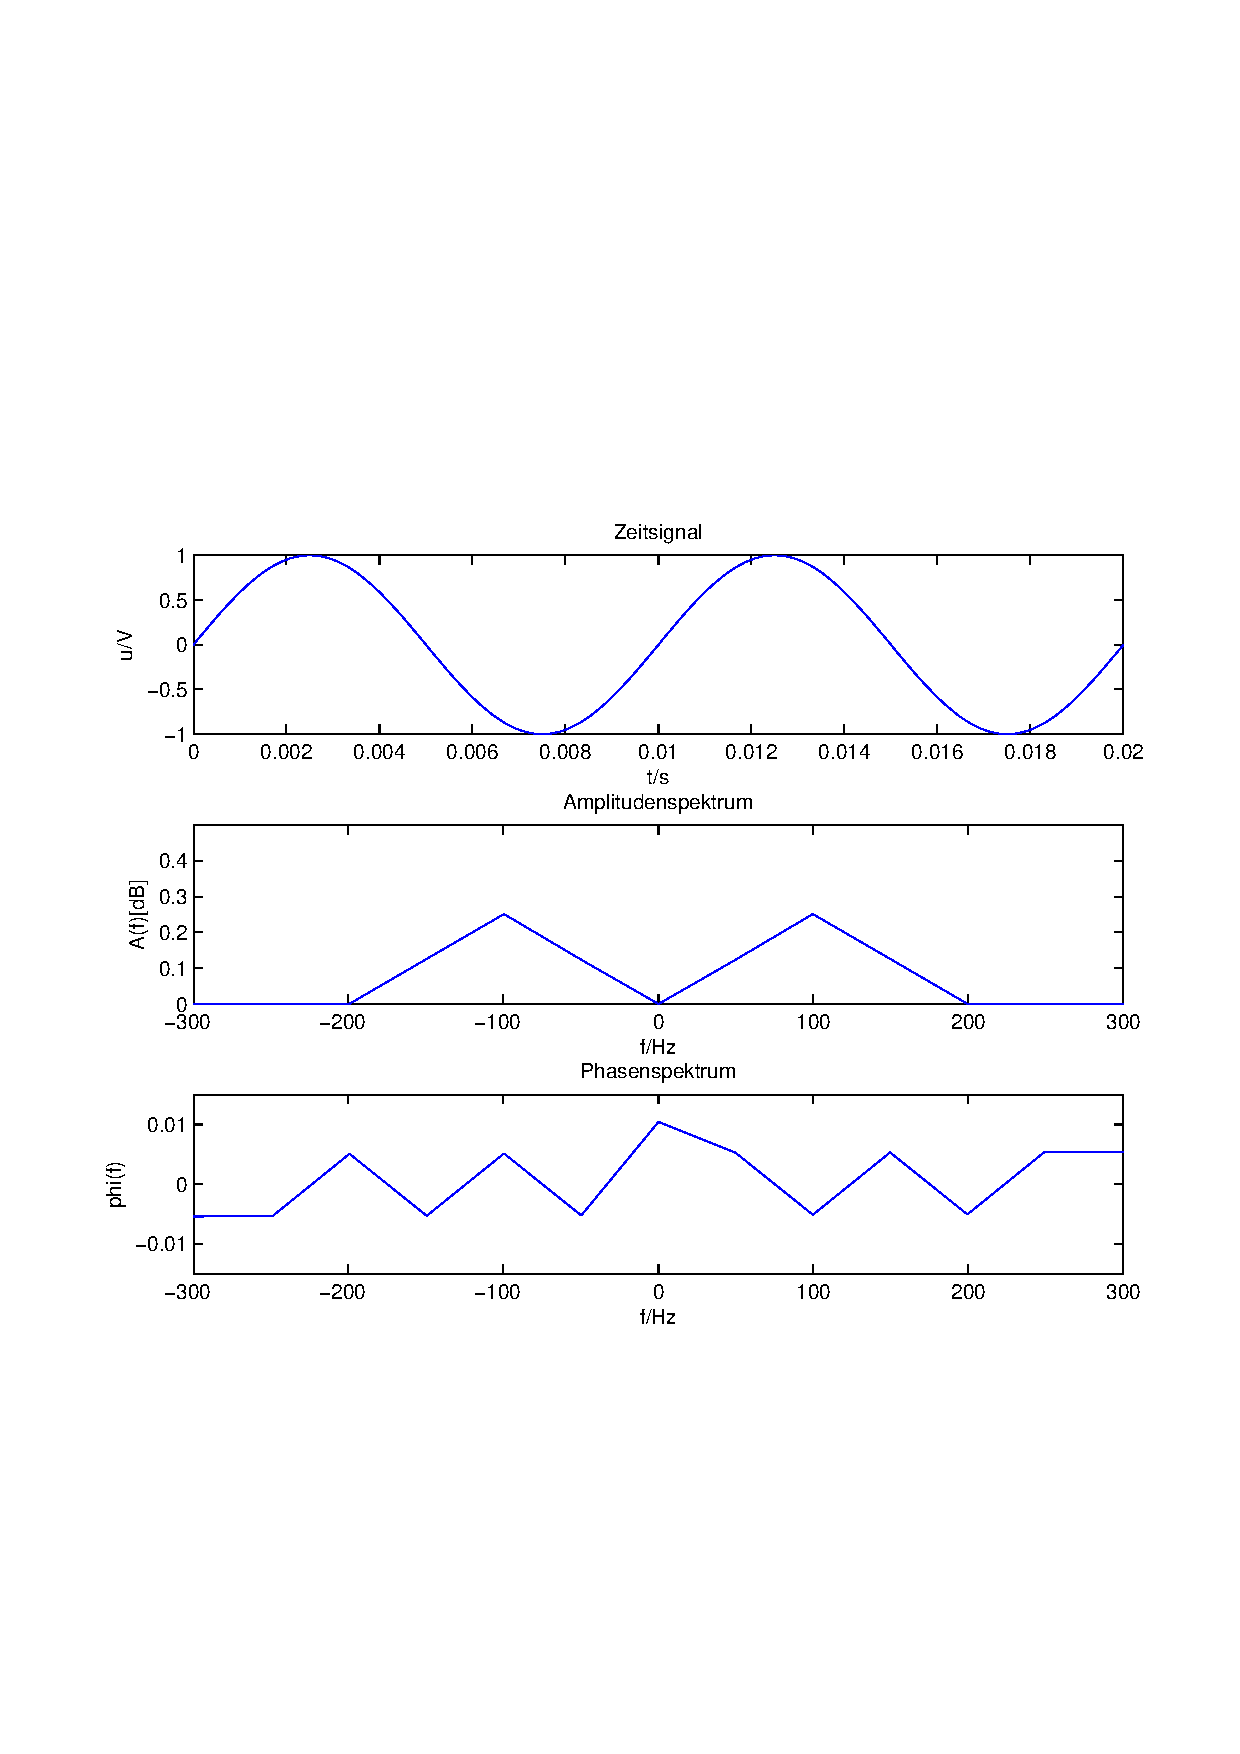
\includegraphics[scale=0.5,trim = 1.5cm 7cm 1.5cm 8cm, clip]{./Bilder/Hanningwindow} %FIXME [width=640px,
                            % height=474px]
                            \caption{DFT eines Rechteckfensters mit Zeropadding}
                        \end{figure}
    
                    \end{minipage}
                    \begin{minipage}{0.6\textwidth}
    
                         \begin{figure}[H]
                            \label{fig:}
                            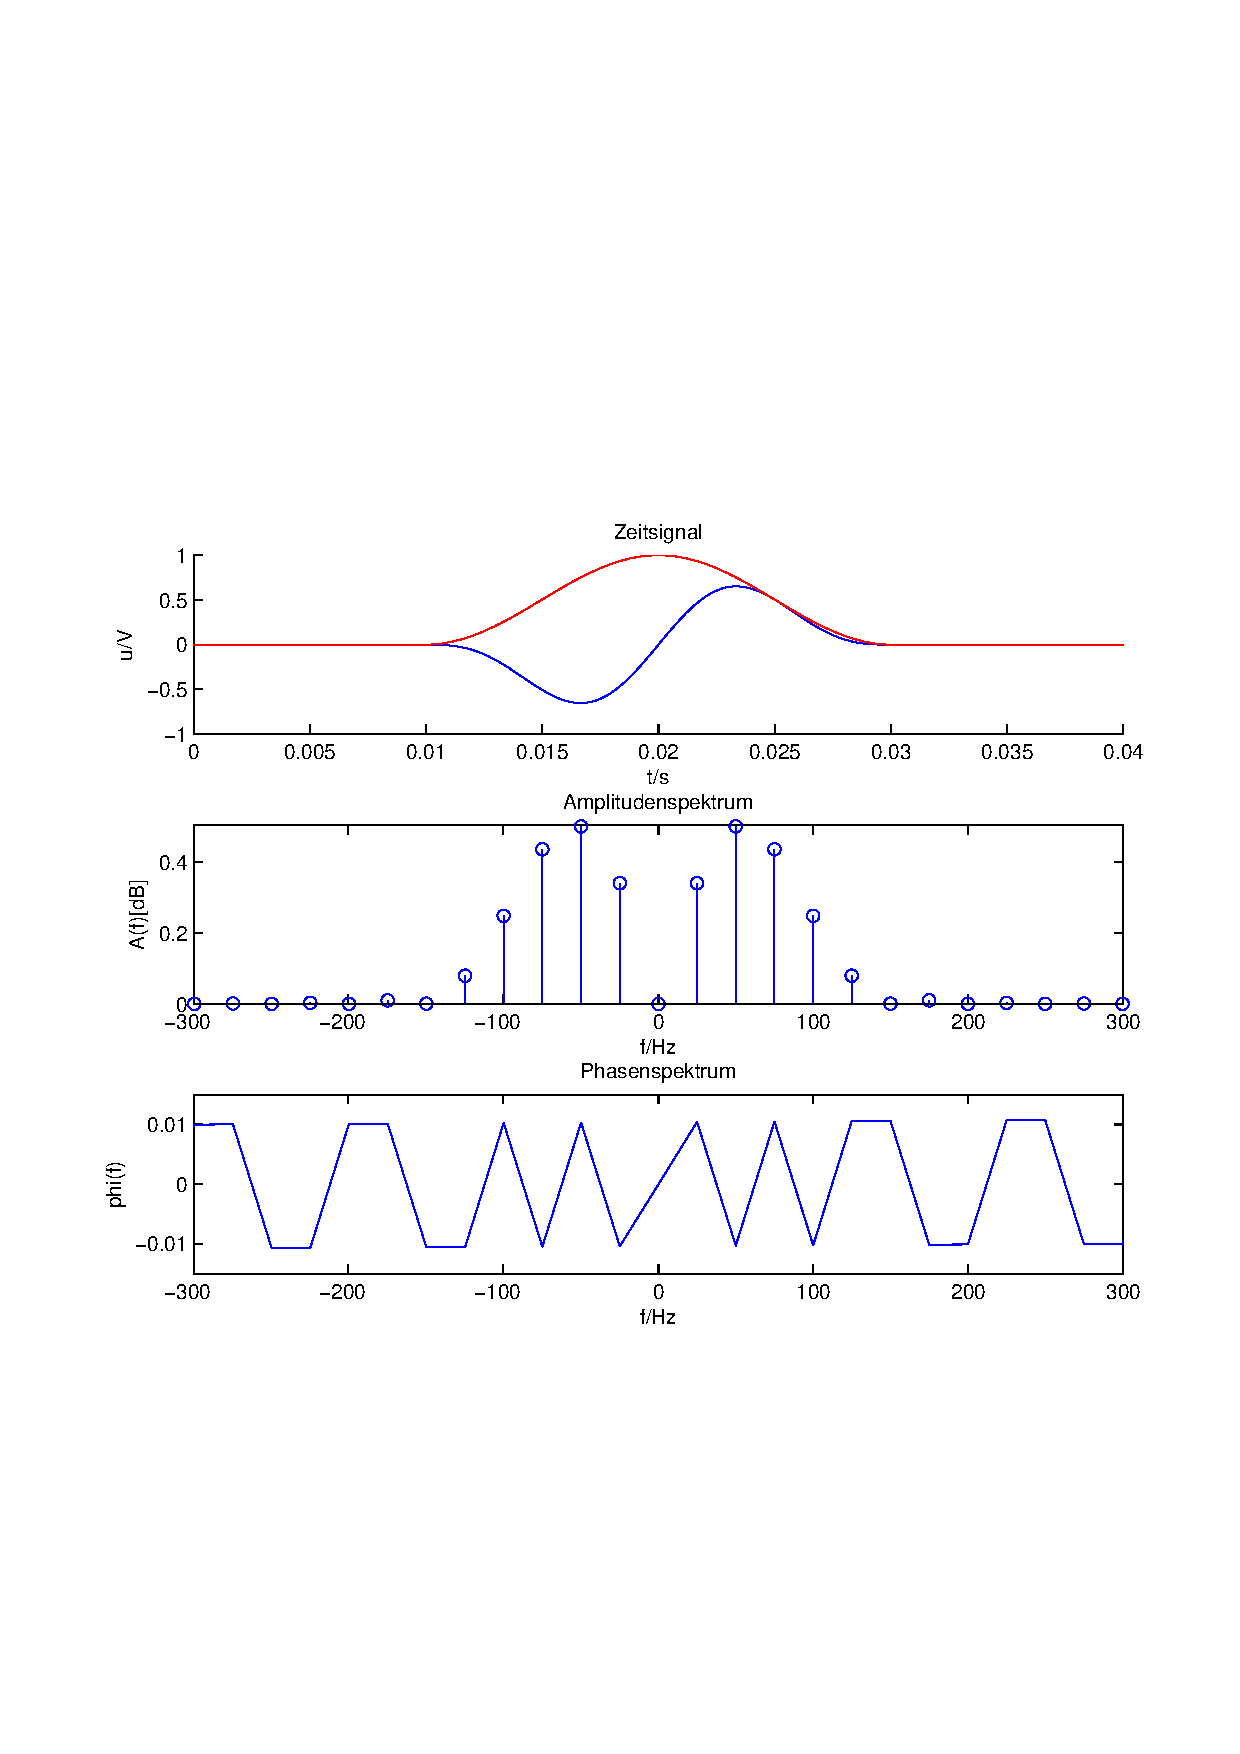
\includegraphics[scale=0.5, trim = 1.5cm 7cm 1.5cm 8cm, clip]{./Bilder/Hanningwindowverkuerzt} %FIXME [width=640px,
                            % height=474px]
                            \caption{DFT eines Hanningfensters mit Zeropadding}
                        \end{figure}
                   \vspace{-1.5em}
    
                    \end{minipage}
    
                \end{tabular}
                \end{center}
   
            Die letzte Simulation zeigt eine Fensterung, die zu dem Leck-Effekt
            führt. Als Ergebniss ist ein beiteres und flacheres Spektrum zu sehen, wie es beim Leckeffekt zu erwarten war.
    			
		\end{quote}

        \subsubsection{DFT eines Rechteck- und Hanningfenster}
		\begin{quote}
            Außerdem untersuchten wir die Spektren von einem Hanning- und einem Rechteckfenster, zuerst mit einer
            Fensterlänge von $16$ und danach mit einer Länge von $2^20$, wobei die restlichen Werte durch Null-Padding
            eingefügt wurden.\\
            Das dazugehörige Skript Vorbereitungsaufgabe43.m befindet sich im Anhang
            Die Plotts dazu sind hier:
            
                %4 Grafiken:
                \begin{center}
                \begin{tabular}{ll}
    
                \hspace{-11em}
                    \begin{minipage}{0.6\textwidth}
    
                        \begin{figure}[H]
                            \label{fig:}
                            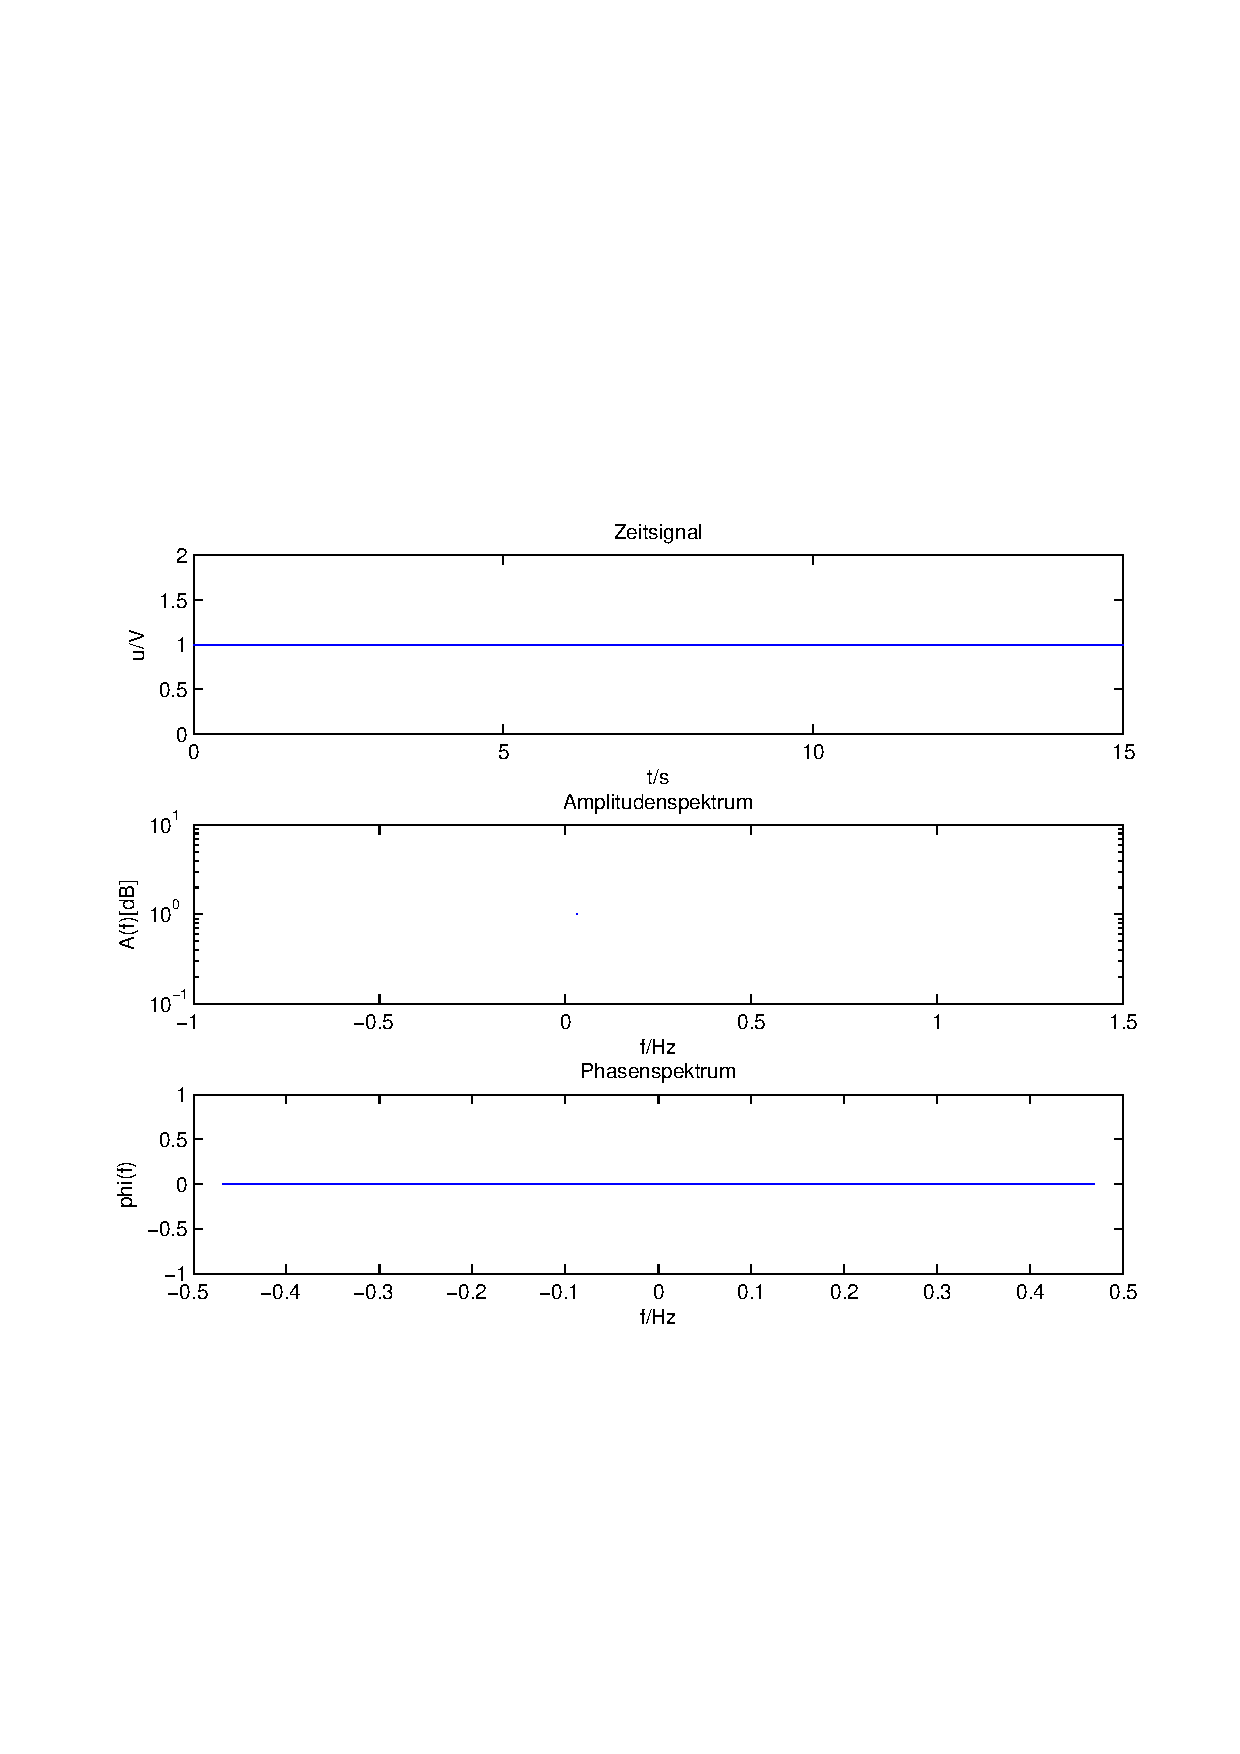
\includegraphics[scale=0.5, trim = 1.5cm 7cm 1.5cm 8cm, clip]{./Bilder/RechteckDFT}
                            %FIXME [width=640px,
                             %height=474px]
                            \caption{DFT eines Rechteckfensters}
                        \end{figure}
    
                    \end{minipage}
                    \begin{minipage}{0.6\textwidth}
    
                        \begin{figure}[H]
                            \label{fig:}
                            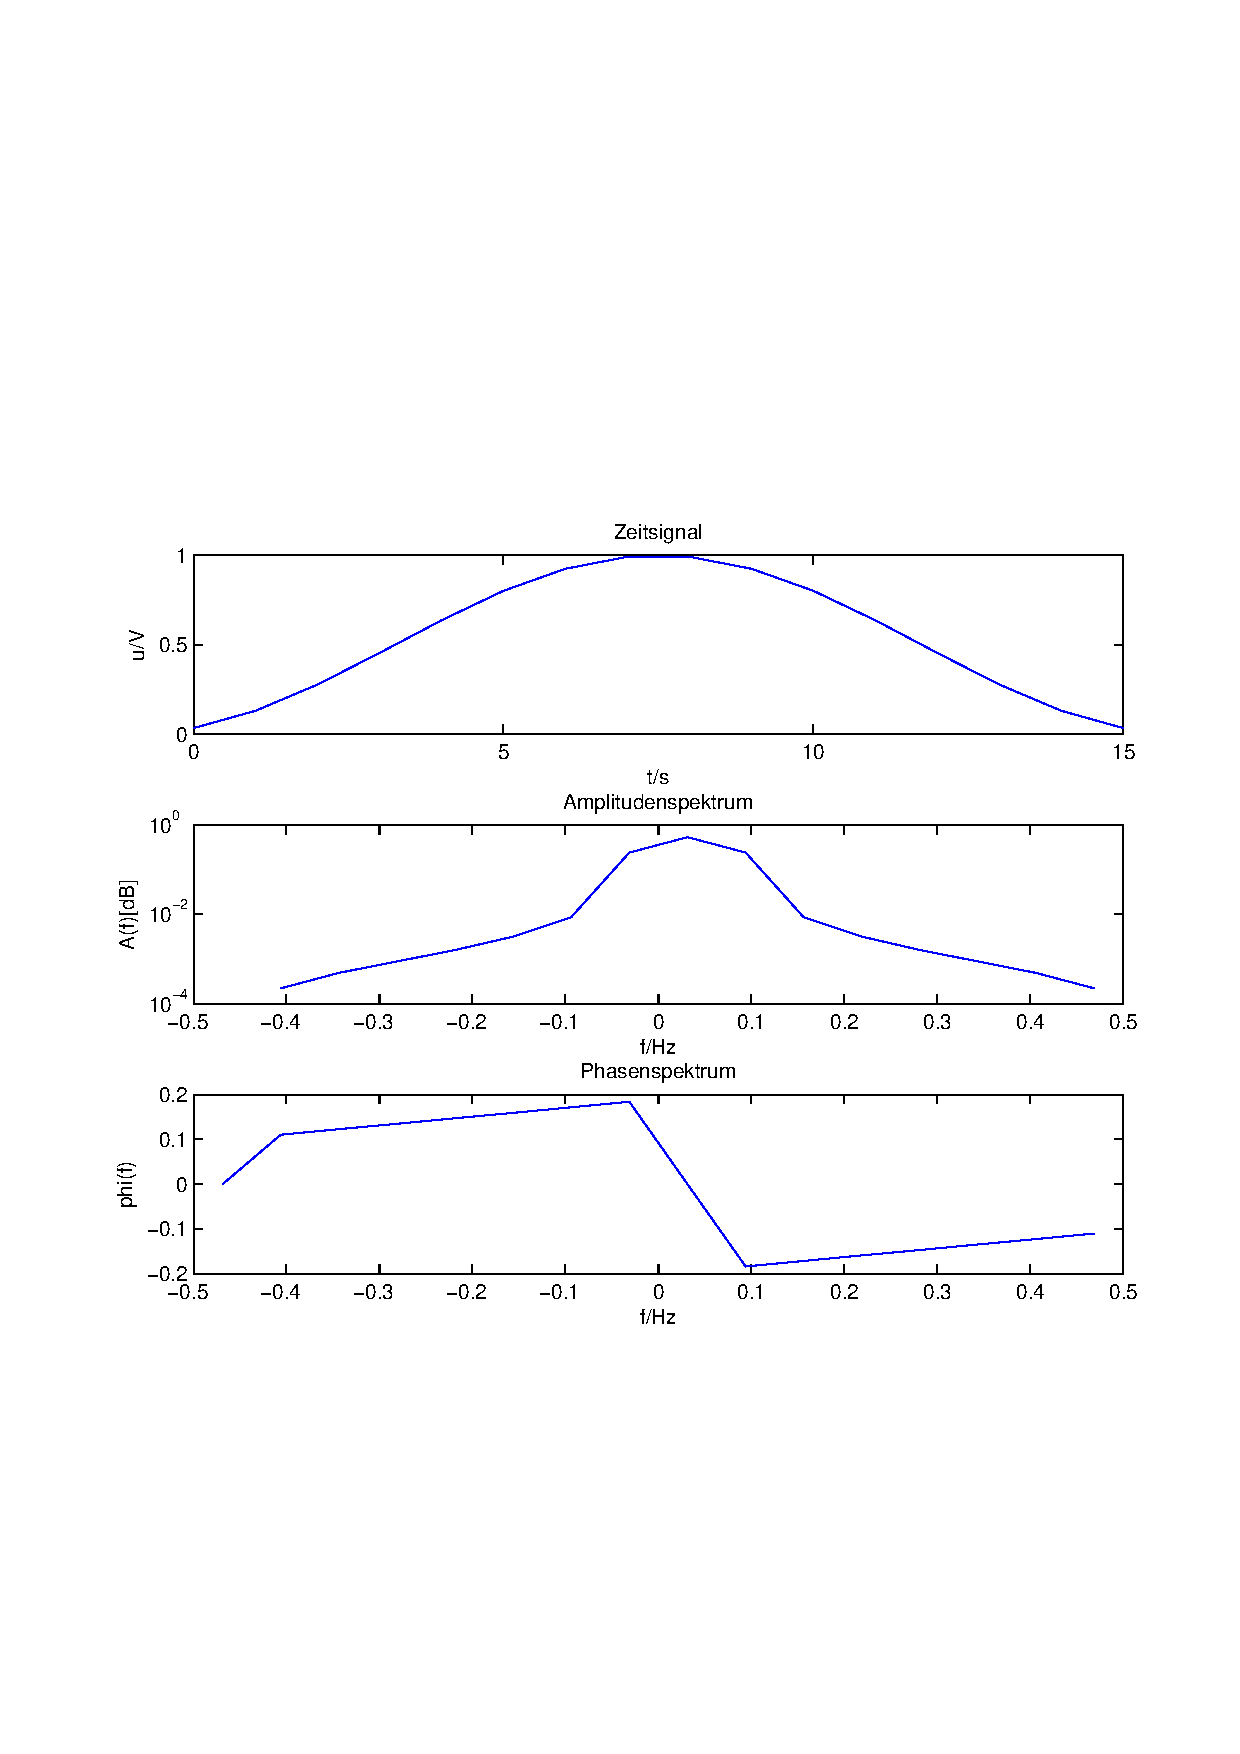
\includegraphics[scale=0.5, trim = 1.5cm 7cm 1.5cm 8cm, clip]{./Bilder/HanningDFT}
                            %FIXME [width=640px,
                             %height=474px]
                            \caption{DFT eines Hanningfensters}
                        \end{figure}
                    \vspace{-1.5em}
    
                    \end{minipage}
    
                \end{tabular}
                \end{center}
    
                            %4 Grafiken:
                \begin{center}
                \begin{tabular}{ll}
    
                \hspace{-11em}
                    \begin{minipage}{0.6\textwidth}
    
                        \begin{figure}[H]
                            \label{fig:}
                            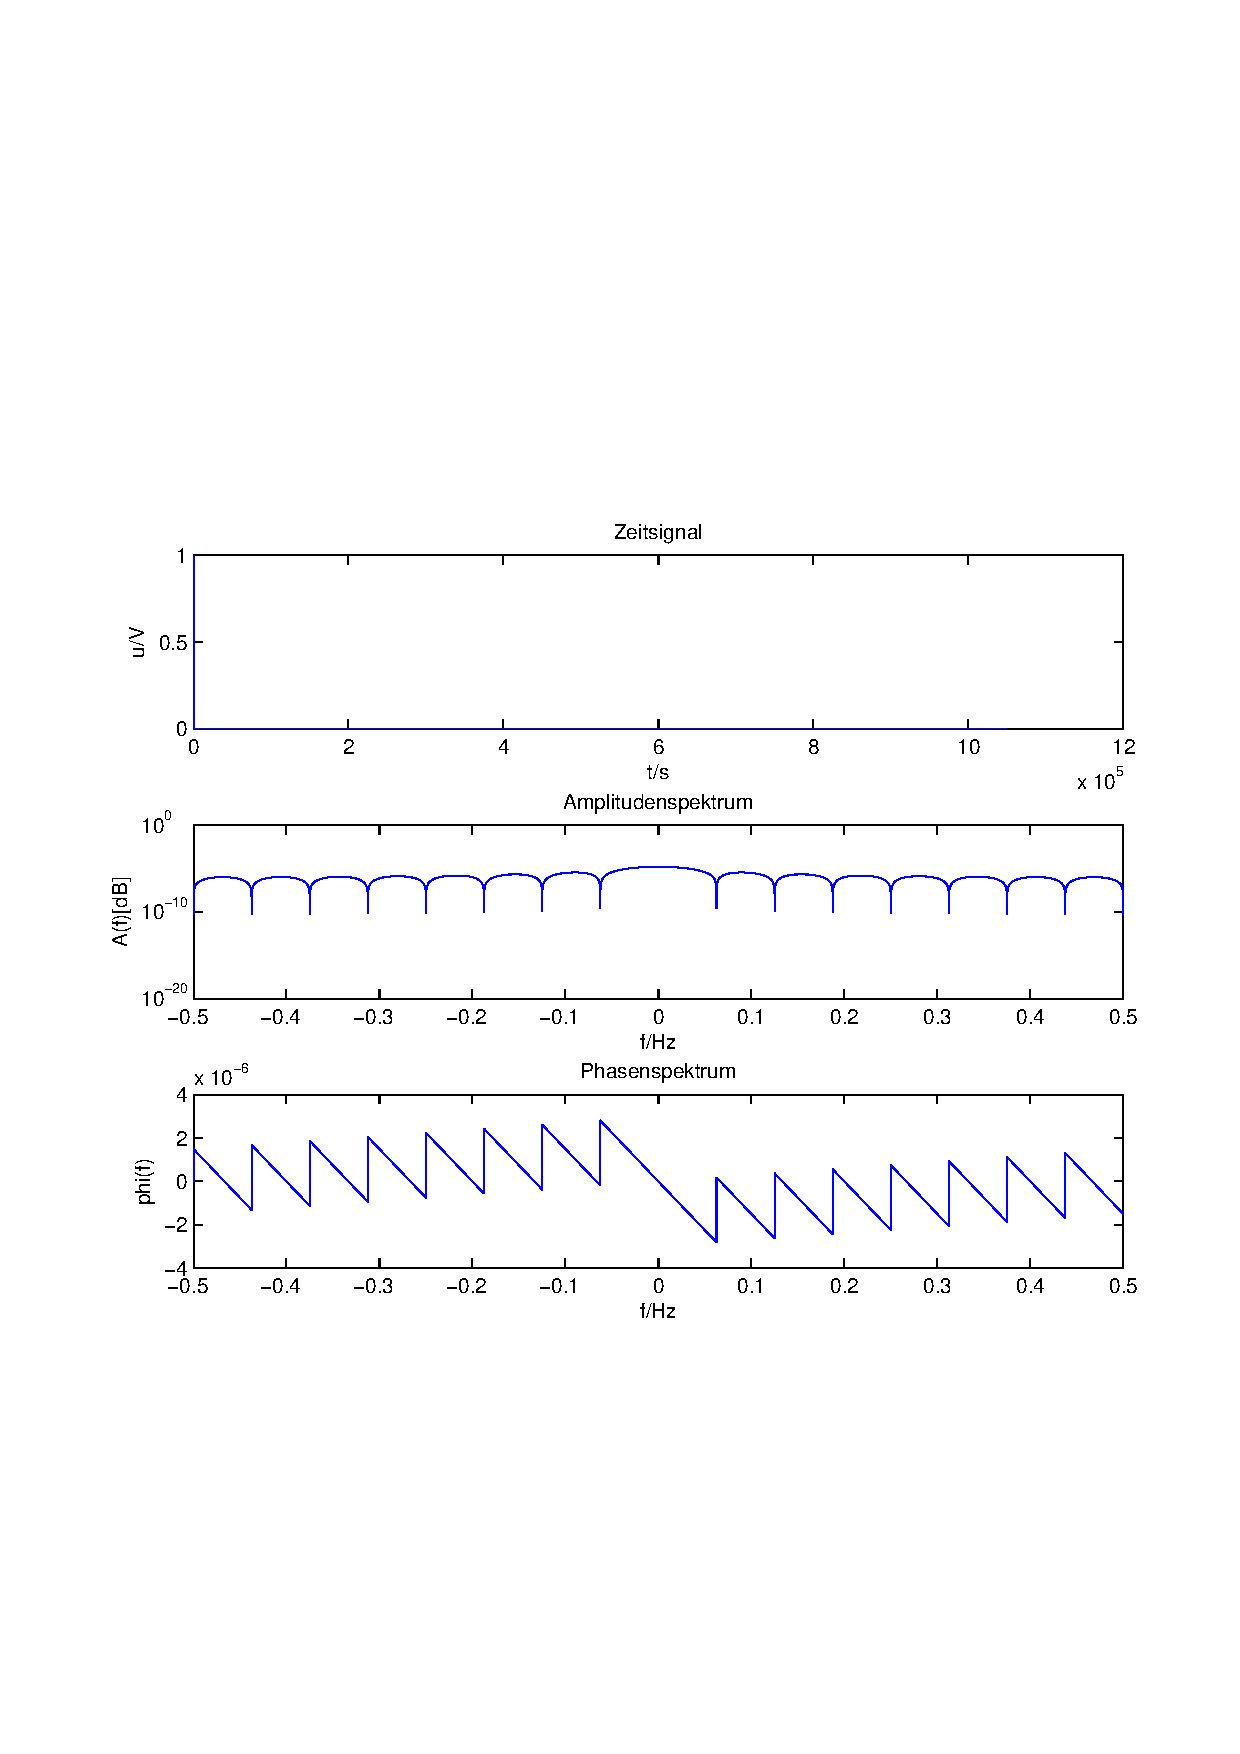
\includegraphics[scale=0.5, trim = 1.5cm 7cm 1.5cm 8cm, clip]{./Bilder/RechteckDFTzeropadding} %FIXME [width=640px,
                            % height=474px]
                            \caption{DFT eines Rechteckfensters mit Zeropadding}
                        \end{figure}
    
                    \end{minipage}
                    \begin{minipage}{0.6\textwidth}
    
                         \begin{figure}[H]
                            \label{fig:}
                            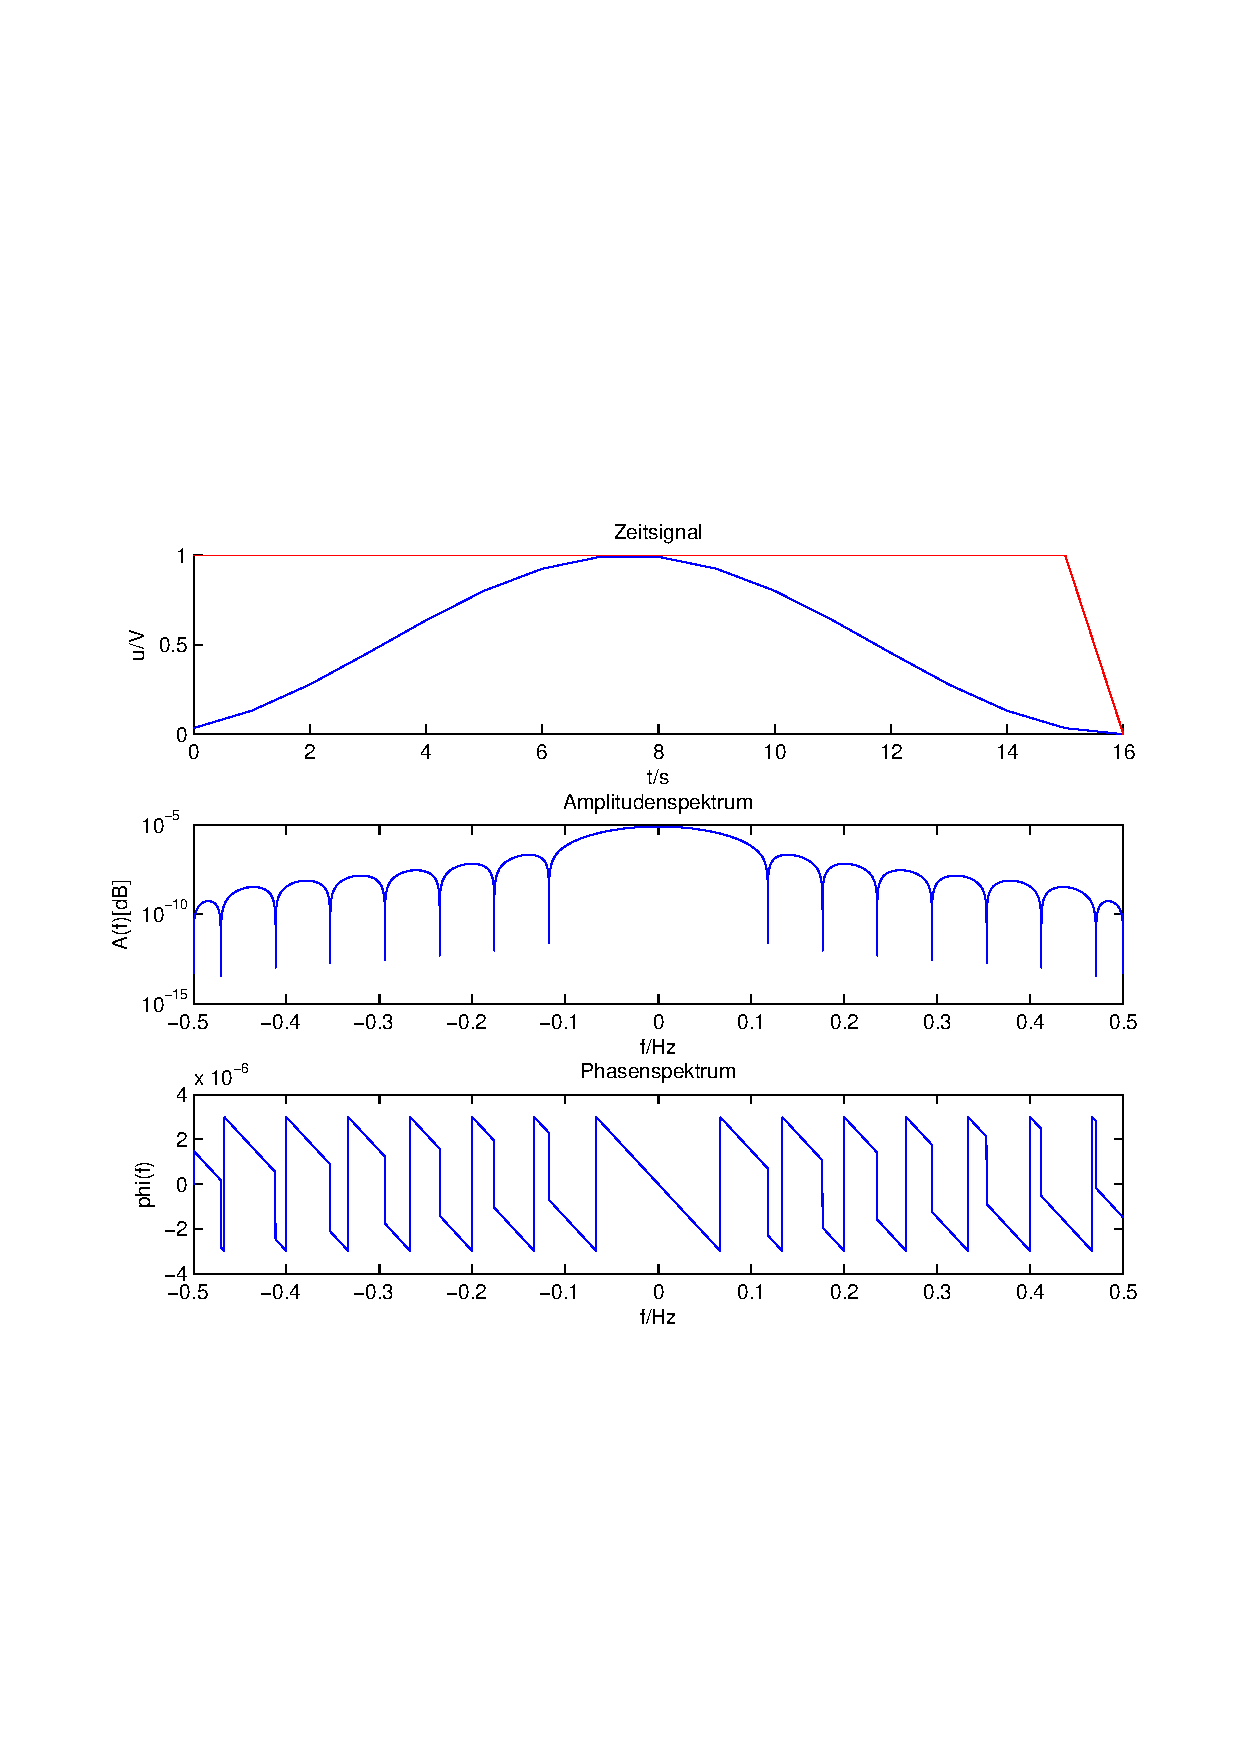
\includegraphics[scale=0.5, trim = 1.5cm 7cm 1.5cm 8cm, clip]{./Bilder/HanningDFTzeropadding} %FIXME [width=640px,
                            % height=474px]
                            \caption{DFT eines Hanningfensters mit Zeropadding}
                        \end{figure}
                   \vspace{-1.5em}
    
                    \end{minipage}
    
                \end{tabular}
                \end{center}
                
        Wir können sehen, dass die DFT-Spektren der Fenster mit dem Zero-Padding
        den erwarteten Sifunkionen entsprechen, während die DFT-Spektren der
        Fenster mit der Länge von $16$ es nicht tun. Dieses Ergebnis liegt
        daran, dass durch die DFT das Zeitsignal periodisch erweitert wird. Wenn
        beispielsweise beim Rechteck ein Signal mit der konstanten Amplitude von
        $1$ unendlich erweitert wird, erhält man ein unendlich ausgedehntes Rechteck mit der
        Amplitude $1$. Bei der DFT wird das Signal dann nicht als das
        Ursprungssignal erkannt und die Spektren weichen von der Erwartung ab.
        Wenn aber durch das Zero-Padding das Rechteck in der unendlichen Periodizität hervorgehoben wird, 
        kann das Signal als Rechteck abgetastet und in eine korrekte Sifunktion transformiert
        werden. Das gleiche Ereignis macht sich auch beim Hanningfenster
        sichtbar. 
            
		\end{quote}
    \end{quote}
\end{quote}

%--------------------------------------------------------------------
%--------------------------------------------------------------------

\section{Termin 3: Spektralanalyse I - DFT}
\begin{quote}

	\subsection{Schaltungsaufbau}
	\begin{quote}
	Im praktischen Teil des dritten Termins wurden nun reelle Messwerte aufgenommen
	und anhand der Diskreten Fouriertransformation untersucht.\\
	Dazu wurde zunächst eine Schaltung aufgebaut, in der der Strom im
	Dimmerschaltkreis erfasst werden konnte. Der Strom aus der Steckdose führt
	dabei in die Dimmerschaltung und dann in den Stromwandler der Wandler-Box. Dort
	wird das Signal in eine Spannung umgewandelt. Das Verhältnis von Strom zu
	Spannung ist bei dem Wandler linear. Bei einem Maximalstrom von $0.9 A$ kann
	man eine Maximalspannung von $\pm 10 V$ erhalten. Daher muss der Vorfaktor von
	$\frac{0.9 A}{10 V} = 0.09 \frac{A}{V}$ berücksichtigt werden. Noch in der
	Wandler-Box wird dieses Signal gefiltert und führt zum Sensorknoten, wo anhand
	der Spannungsmessung Rückschlüsse auf den Strom gemacht werden können.
	
	\begin{figure}[H]
    \centering
        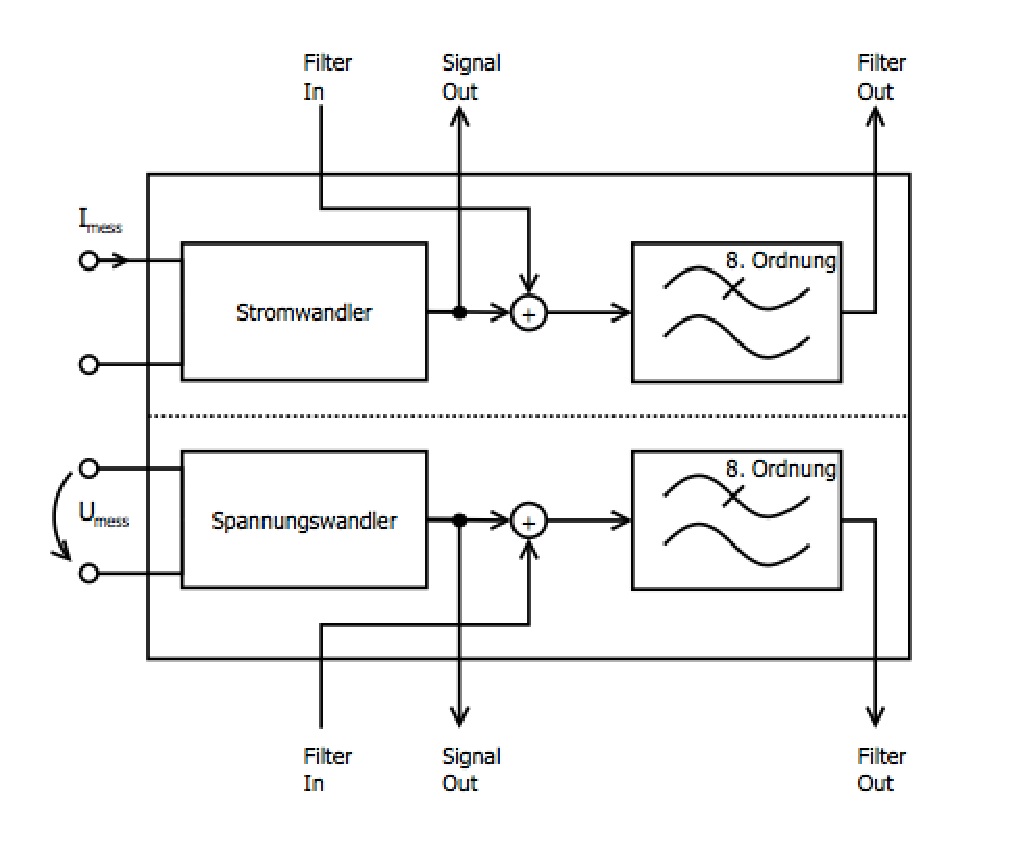
\includegraphics[scale=0.7, trim = 0cm 0cm 0cm 0cm, clip]{./Bilder/Schaltungwandlerbox}
            \caption{Aufbau Wandlerbox}
    \end{figure}
    
	\cite{Schaltungwandlerbox}
	\end{quote}
	
	\subsection{MATLAB-Skript für Anschnittswinkel-Bestimmung}
	\begin{quote}	
	Als nächstes soll anhand eines selbstgeschriebenem MATLAB-Skripts der
	Anschnittswinkel der unterschiedlichen Signale bestimmt werden. Die
	Anschnittswinkel werden dafür vorher mit dem Oszilloskop eingestellt. Da es
	manuell nicht so einfach ist, wurden kleine Abweichungen toleriert.
	
	Unsere anhand des MATLAB-Skripts errechneten Werte wichen nur minimal von den
	erwarteten Anschnittswinkeln ab. Das Ergebnis war also zufriedenstellend. 
    Das dazugehörige Skript ist am Ende des Protokolls zu sehen.
   	\end{quote}
	
	\subsection{Amplituden- und Phasenspektrum des Stroms anhand der DFT}
	\begin{quote}
        In diesem Teil bestand die Aufgabe darin für einen selbst gewählten Anschnittswinkel den Stromverlauf
        aufzunehmen und das Amplituden sowie das Phasenspektrum aufzunehmen. Es sollte eine passende Abtastfrequenz und
        ein passendes Messfenster gewählt werden. Außerdem sollte der Einfluss des Antialiasing-Filters auf den
        Betragsfrequenzgang korrigiert werden.\\
        Für unsere Messung haben wir uns entschieden, mit einer Abtastfrequenz
        von $15kHz$ und einem Messfenster von $600$ Messwerten abzutasten. Die
        Abtastfrequenz haben wir gewählt, da sie fast die maximal mögliche Abtastfrequenz des Messknotens ist und wir mit 
        mehr Abtastwerten eine größere Genauigkeit erreichen. 
        Als Zeitfenster haben wir zwei Perioden gewählt, was bei einer Frequenz von $50Hz$ ein Zeitfenster von $0$ bis
        $0.04 s$ bedeutet. Bei der gewählten Abtastfrequenz ergibt sich daraus ein Messfenster von $600$
        Messwerten.
        
        \vspace{1em}
        
        Um die Auswirkung des Antialiasing-Filters auf den Betragsfrequenzgang
        zu korrigieren, betrachen wir zunächst den Betragsfrequenzgang des
        Filters selbst, den wir in einem früheren Termin aufgenommen haben. Wie gewollt dämpft das Filter alle Frequenzen 
        größer als $5kHz$ mit mehr als $60dB$ und ist damit nicht mehr von dem ADU messbar.
        Um dieses Ziel zu erreichen, beginnt das Filter schon ab einer Frequenz
        von $1,2 kHz$ zu dämfen und verfälscht dadurch die Amplituden der Messwerte der Frequenzen 
        zwischen $1,2 kHz$ und $5 kHz$.
        
        \vspace{1em}
        
        Diesen Fehler korrigieren wir indem wir den Kehrwert des Amplitudengangs des Filters mit dem Betragsspektrum der
        Messwerte multiplizieren. Dafür benötigen wir genau so viele Abtastwerte
        des Amplitudengangs des Filters wie wir auch für die gesamte Messung gewählt haben: $600$. 
        Bei der manuellen Messung des Frequenzganges haben wir jedoch
        lediglich $18$ Messwerte aufgenommen. Unser erster Gedanke war eine Interpolation des gemessenen Frequenzgang zu
        erstellen und daraus einen passenden Vektor zu realisieren. Leider
        hatten wir dabei einige Umsetzungsschwierigkeiten, wesshalb uns unser
        Tutor den Tipp gab, anstatt des reell gemessenen Filters das simulierten
        Filter zu benutzen.\\
        Daher haben wir uns mit Hilfe des bode Befehls den Betragsgang des simulierten Butterworth Tiefpass 8.Ordnung
        für die selben Frequenzen ausgeben lassen, mit denen auch abgetastet
        wurde. Jedoch mussten wir noch beachten, dass das abgetastete Signal bei der DFT doppelt vorkommt 
        und auch den Betragsgang daran anpassen müssen. Da wir
        uns dafür entschieden haben in $dB$ zu arbeiten, haben wir diesen
        Betragsgang von $1$ abgezogen um den invertierten Betragsfrequenzgang zu bekommen.\vspace{1em}
        
        Zur Korrektur haben wir diesen invertierten Betragsfrequenzgang bei der
        Berechnung des Spektrum des gemessenen Signals an das errechnete
        Betragsspektrum addiert. Anschließend haben wir das korrigierte Spektrum geplottet.
        Außerdem haben wir den korrigierten und den unkorrigierten Betragsfrequenzgang übereinandergelegt.\\
        Hier sind die Ergebnisse:\\
        
        \begin{figure}[H]
        \centering
            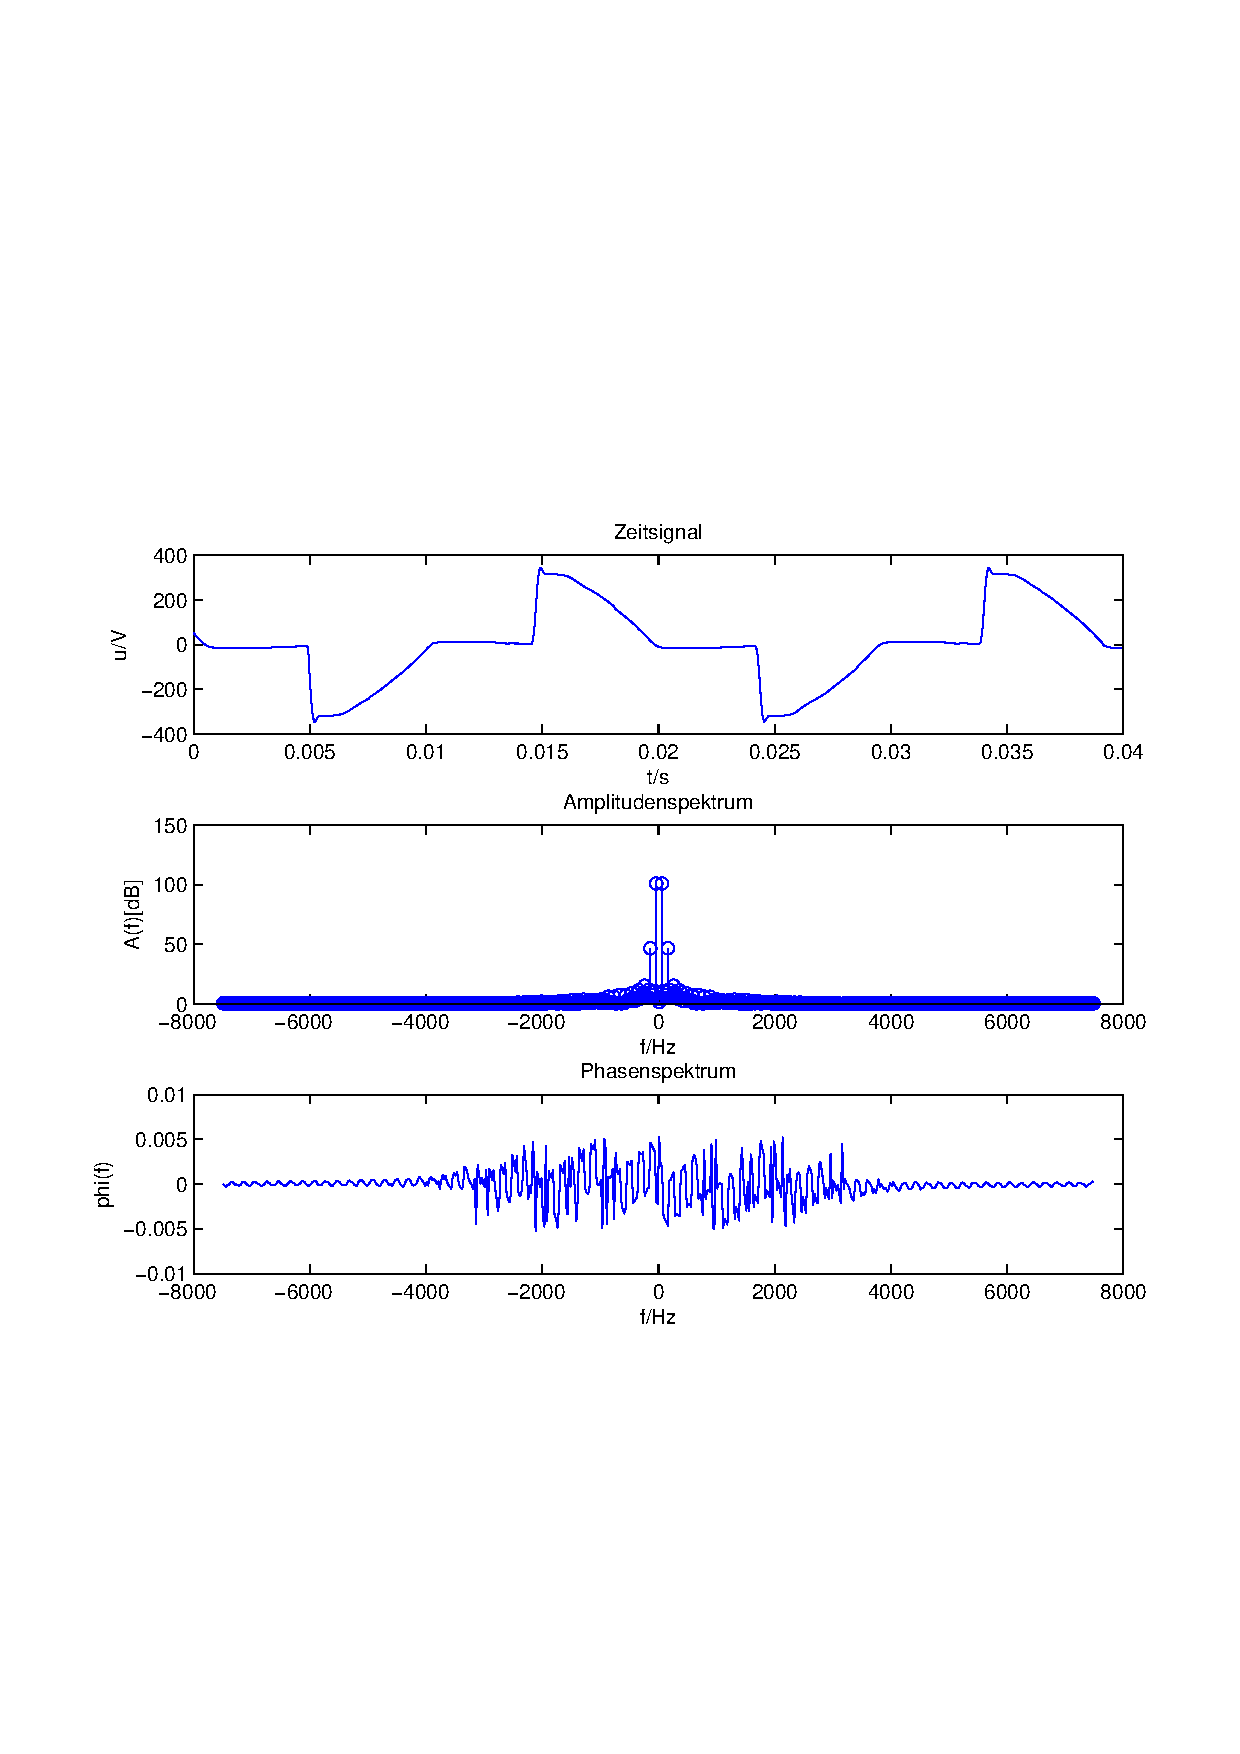
\includegraphics[scale=0.7, trim = 1.5cm 7cm 1.5cm 8.5cm, clip]{./Bilder/korrigiertesSpektrumauf33}
                \caption{korregiertes Spektrum des aufgenommenen Stromverlaufs}
        \end{figure}

        \begin{figure}[H]
        \centering
            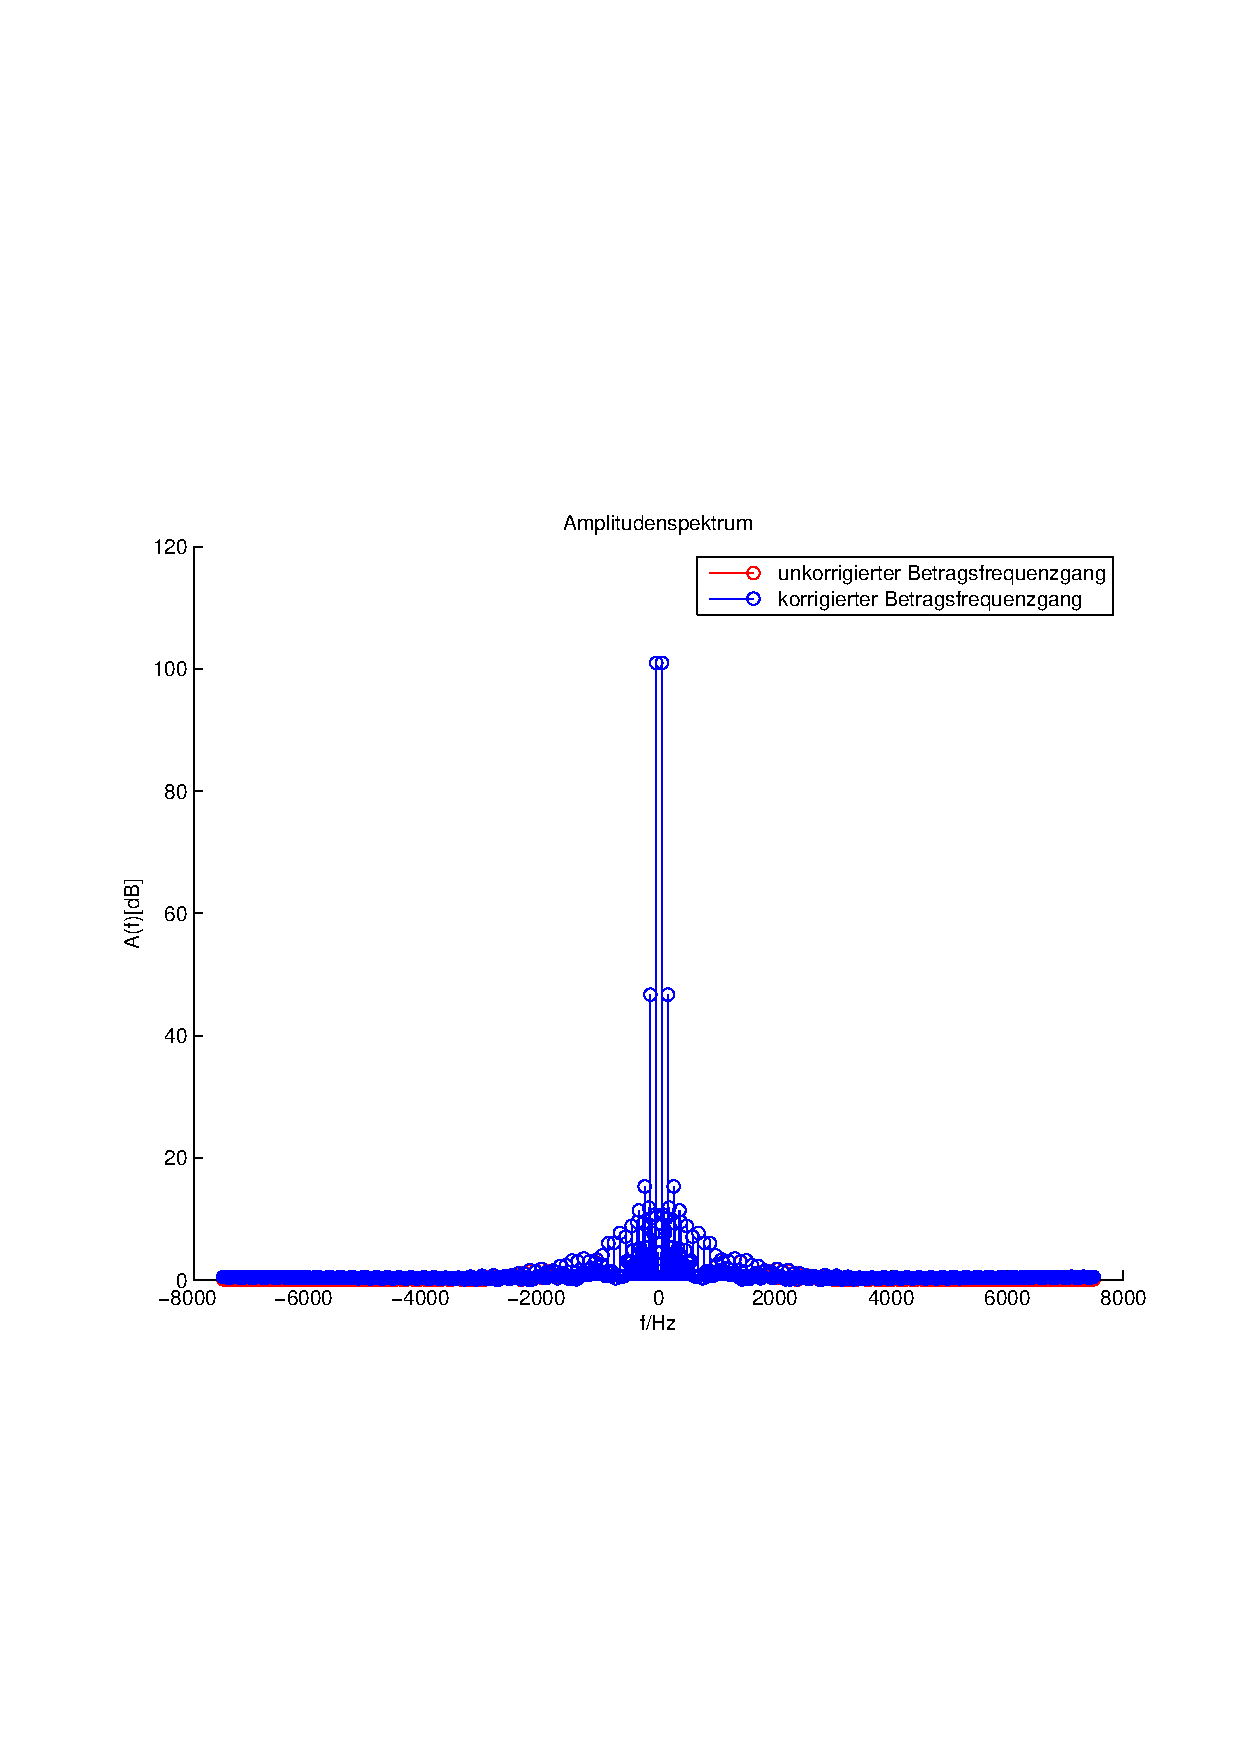
\includegraphics[scale=0.7, trim = 1.5cm 7cm 1.5cm 8.5cm, clip]{./Bilder/betragsfrequenzgang_korr_vs_unkorr.pdf}
                \caption{Korregierter und unkorrigierter Betrgsfrequenzgang}
        \end{figure}
        
        Wie zu erwarten war hat die Korrektur auf den ersten Blick keinen auffallenden Einfluss. Das Betragspektrum
        zeigt, dass die Frequenzen, die durch das Antialiasing Filter
        beeinflusst werden, sowieso schon eine kleine Amplitude besitzen. Um jedoch die Auswirkungen der Korrektur 
        genauer zu betrachten, Vergrößern wir den Betragsfrequenzgang auf den interessanten Bereich der hohen Frequenzen.
        
        \begin{figure}[H]
        \centering
            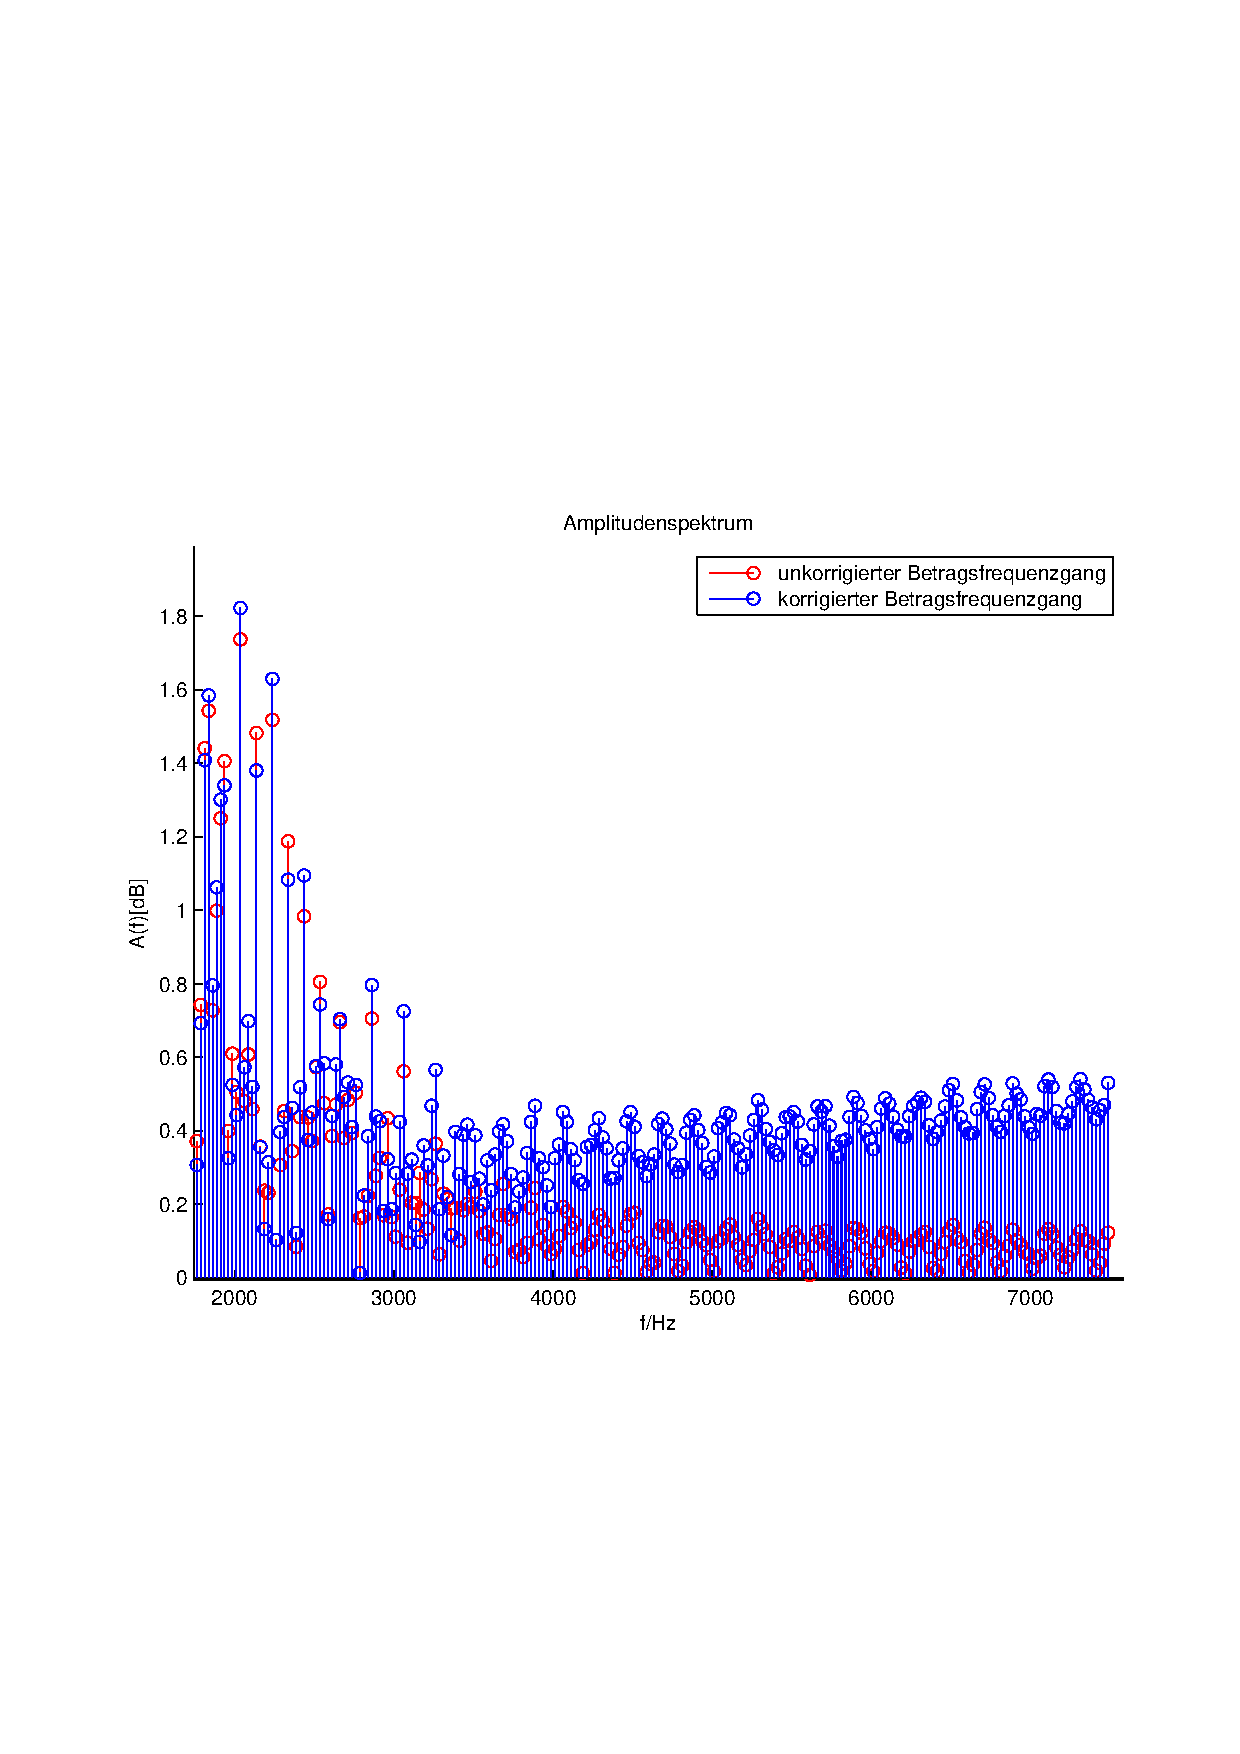
\includegraphics[scale=0.7, trim = 1.5cm 7cm 1.5cm 8.5cm,
            clip]{./Bilder/betragsfrequenzgang_korr_vs_unkorr_zoom}
                \caption{Korregierter und unkorrigierter Betragsfrequenzgang}
        \end{figure}
    
        In dieser Grafik lässt sich gut erkennen, dass die Korrektur die
        Amplituden der hohen Frequenzen verstärkt, die Amplituden der niedrigen Frequenzen 
        jedoch nahezu unverändert lässt. Ein solches Verhalten haben wir erwartet.
        
	\end{quote}
	
	\subsection{Effektivwert des Stroms im Zeit- und Frequenzbereich}
	\begin{quote}
	Zuletzt sollte der Effektivwert des Stroms einer Messung im Zeit- und
	Frequenzbereich ermittelt werden, indem der MATLAB-Skript der
	Vorbereitungsaufgabe verwendet wurde. Wir verwendeten den Strom des Signals bei
	einem Anschnittswinkel von $\frac{\pi}{2}$.\\
	Das MATLAB-Skript gibt uns das Ergebnis von $0.21 A$ für Zeit- und
	Frequenzbereich. Der mithilfe des Multimeters gemessene Strom beträgt $0.224
	A$.\\
	
	Vergleicht man beide Messungen, kann man sehen, dass es keine erhebliche
	Differenz gibt.
	
	 
	\end{quote}
\end{quote}

\section{Termin 4: Spektralanalyse II - Fensterung}
\begin{quote}

	Im Labor soll nun ein phasenangeschnittener Strom gemessen und mit der DFT untersucht werden.
	Dazu wird der Dimmer auf dem "Lampenbrett" verwendet.
	
	\subsection{Versuchsaufbau}
	\begin{quote}
    	Allgemein gilt: Um Strom zu messen muss man ein Amperemeter in Reihe mit der Last schalten. 
    	Daher muss auch hier der Stromwandler aus der "blauen Box" in Reihe zur Last geschaltet 
    	werden. Das in eine Spannung gewandelte und gefilterte Signal wird mit dem Sensorknoten gemessen. 
    	Das Messsignal wird anschließend mit Matlab weiterverarbeitet.
    
    	\begin{figure}[htb]
        	\centering
        	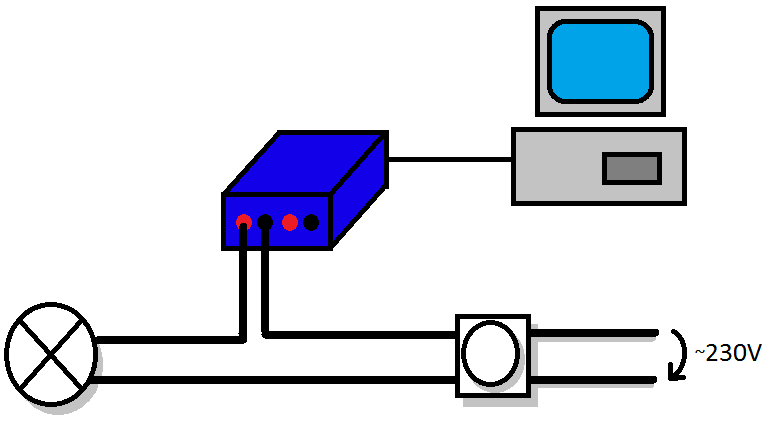
\includegraphics[scale=0.6,  trim = 0cm 0cm 0cm 0cm,clip]{./Bilder/Versuchsaufbau1}
        	\caption{Versuchsaubau um angeschnittenen Strom zu messen}
    	\end{figure}	
	\end{quote}
	
	\subsection{Versuchsdurchführung}
	\begin{quote}
		        
		\subsubsection{Spektrum mit Fensterung}
		\begin{quote}
            An dem Phasenanschnittdimmer wird ein Zündwinkel eingestellt. Dieser kann aber nicht am Dimmer bestimmt
            werden, da eine Skala fehlt. Statt dessen wird das Phasenangeschnittene Signal zunächst mit dem Ossziloskop
            gemessen.
            Dabei wird die Zeitdifferenz zwischen dem Nulldurchgang und Zündmoment gemessen. Anschließend wird das
            Signal auch mit dem Sensorknoten abgetastet.\\
            Um den Leckeffekt von vornerein zu umgehen, wird als Messdauer ein ganzzahliges vielfaches der Signalperiode
            (20ms) gewählt.\\
            Die Abtastfrequenz muss wie folgt gewählt werden.
            Die 3dB-Grenzfrequenz des Allaisingfilters liegt bei 2,05kHz, die Auflösung des ADUs beträgt 10Bit und der
            Eingangsspannungsbereich beträgt 14V.\\
            
            \begin{align}
                U_{LSB} = \frac{14V}{2^{10}-1} = 0,01368V 
            \end{align} 
		
		    Nun kann die benötigte Dämpfung, um Allaising zu verhindern, berechnet werden.\\
		
            \begin{align}
                D = 20 \cdot log_{10}(\frac{14V}{U_{LSB}}) = 60dB
            \end{align} 
		
            Der Filter ist ein Filter 8.Ordnung und besitzt eine Steilheit von 160dB/Dekade. Es wird abgeschätzt, dass
            der Filter ab ca.7kHz um über 60dB dämpft. Daher muss die Abtastfrequenz mindestens 14kHz betragen.

    		
    		\TODO{Özgü: Fensterwahl: Hanning oder Rechteck im Vergleich, da beide
    		Fensterfunktionen ihre pros und cons für die DFT Spektren haben(siehe Skript).
    		Abtastfrequenz 15kHz, da nahezu höchste Auflösung des Messknotens, also größer
    		als 7kHz (num of samples beträgt 600). Wir haben 0.04s aufgenommen, also genau zwei Periodendauer a 20ms. 
    		Länge des Fensters beträgt ein ganzzahliges Vielfaches der Periodenlänge des
    		Signals.}
		
		\end{quote}
		
		\subsubsection{Auswirkungen des Fensters}
		\begin{quote}
		  Es werden nun nacheinander Rechteck-, Hanning- und Blackmanfenster über das Signal gelegt. Die Längen der Fenster
		  sind absichtlich so gewählt, dass es zum leckeffekt kommt. Es wird nun untersucht, wie sich die unterschiedlichen
		  Fenster auf den Leckeffekt auswirken.		
		\end{quote}
		
		\subsubsection{Qualität der Netzspannung}
		\begin{quote}
            Nun soll die Qualität der Netzspannung überprüft werden. Theoretisch beträgt die Netzspannung 230V bei 50Hz.
            Allerdings können auf der Grundwelle zusätzlich zu den 50Hz weitere Oberwellen vorhanden sein. Der Anteil
            dieser Oberwellen an der Versorgungsspannung darf nicht über $8\%$ liegen.\\
            Für diesen Versuch wird die Netzspannung an den Spannungswandler der Blauenbox angelegt. Nun kann mit dem
            Sensorknoten die Netzspannung gemessen werden. Der Spannungswandler setzt die Eingangsspannung um den Faktor
            56,6 herrab. Um die Netzspannung zu bestimmen, muss der Messwert mit 56,6 multipliziert werden.
		
    		\begin{figure}[htb]
        		\centering
        		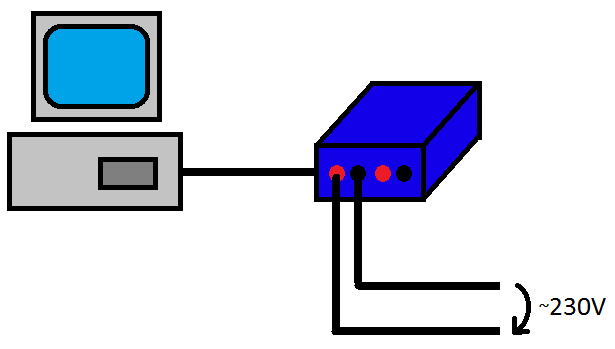
\includegraphics[scale=0.6, trim = 0cm 0cm 0cm 0cm,
                    clip]{./Bilder/Versuchsaufbau2}
        		\caption{Versuchsaubau um Netzqualität zu messen}
    		\end{figure}
		
		Der Gesamtoberschwingungsgehalt (THD-Wert für Total Harmonic Distortion) wird
		anhand folgender Formel berechnet:
		
		\begin{align}
		THD = \frac{\sqrt{U_2^2 + U_3^2 + \cdot \cdot \cdot + U_N^2}}{U_1}
		\end{align} 
		
		Mit diesem Ansatz sollte ein Netzoberschwingungsanalysator auf Basis der DFT
		realisiert werden. Hierzu wurde eine Messkette entworfen.
		
		\end{quote}%Ende subsubsection
	\end{quote}%Ende subsection
	
	\subsection{Versuchsauswertung}
    \begin{quote}
        \subsubsection{Spektrum mit Fensterung}
		\begin{quote}
            Von dem aufgezeichenteten Verlauf des phasenangeschnittetenen Stroms soll das Frequenz- und das
            Phasenspektrum bestimmt werden. Bei der Auswertung ist darauf zu achten, dass das Spektrum nicht durch
            schlechte Wahl des Fensters und der
            Messdauer verfälscht wird.\\
            Der Leckeffekt wird umgangen, indem die Messdauer ein ganzzahliges Vielfaches der Signalperiode beträgt. Die
            Messdauer wurde zu 40ms gewählt. Dies ist die zweifache Periode der Grundwelle.\\
            Es sollen pro Periode 300 Samples aufgenommen werden, um den Verlauf des Signals gut zu verfolgen.
            Daraus ergibt sich folgende Samplerate.
            
            \begin{align}
              f_{Samplerate} = \frac{T_{Messdauer}}{N_{Messwerte}} = 15000Hz
            \end{align} 
            
            Die Mindestsamplerate beträgt 14kHz. Eine Abtastrate von 15kHz ist also ausreichen um das Signal
            alliasingfrei abzutasten.\\
            Als Fenster wird das Hanningfenster gewählt. Es hat ein breites Hauptmaxima. Dadurch wird der Leckeffekt
            stark unterdrückt. Allerdings ist es nicht sehr frequenzselektiv. Dies ist in diesem Fall aber nicht von
            großer Bedeutung, da laut der Simulation (Vorbereitungsaufgaben Termin 3) die wichtigen Frequenzanteile ca.
            50Hz von einander entfernt sind.\\
            Das Spektrum des Signals müsste nun halbwegs vom Leckeffekt befreit sein.
            Allerdings sind die Amplituden durch den Frequenzgang des Antiallaisingfilters und durch die Fensterfunktion
            verzerrt. Um den Frequenzgang des Filters zu kompensieren, wird das Spektrum mit dem inversen Frequenzgang
            korrigiert. Die Verzerrung durch das Fenster kann korrigiert werden, indem das Spektrum durch die Summe des
            Fensters geteilt wird.\\
            
            \begin{figure}[H]
                \centering
                
                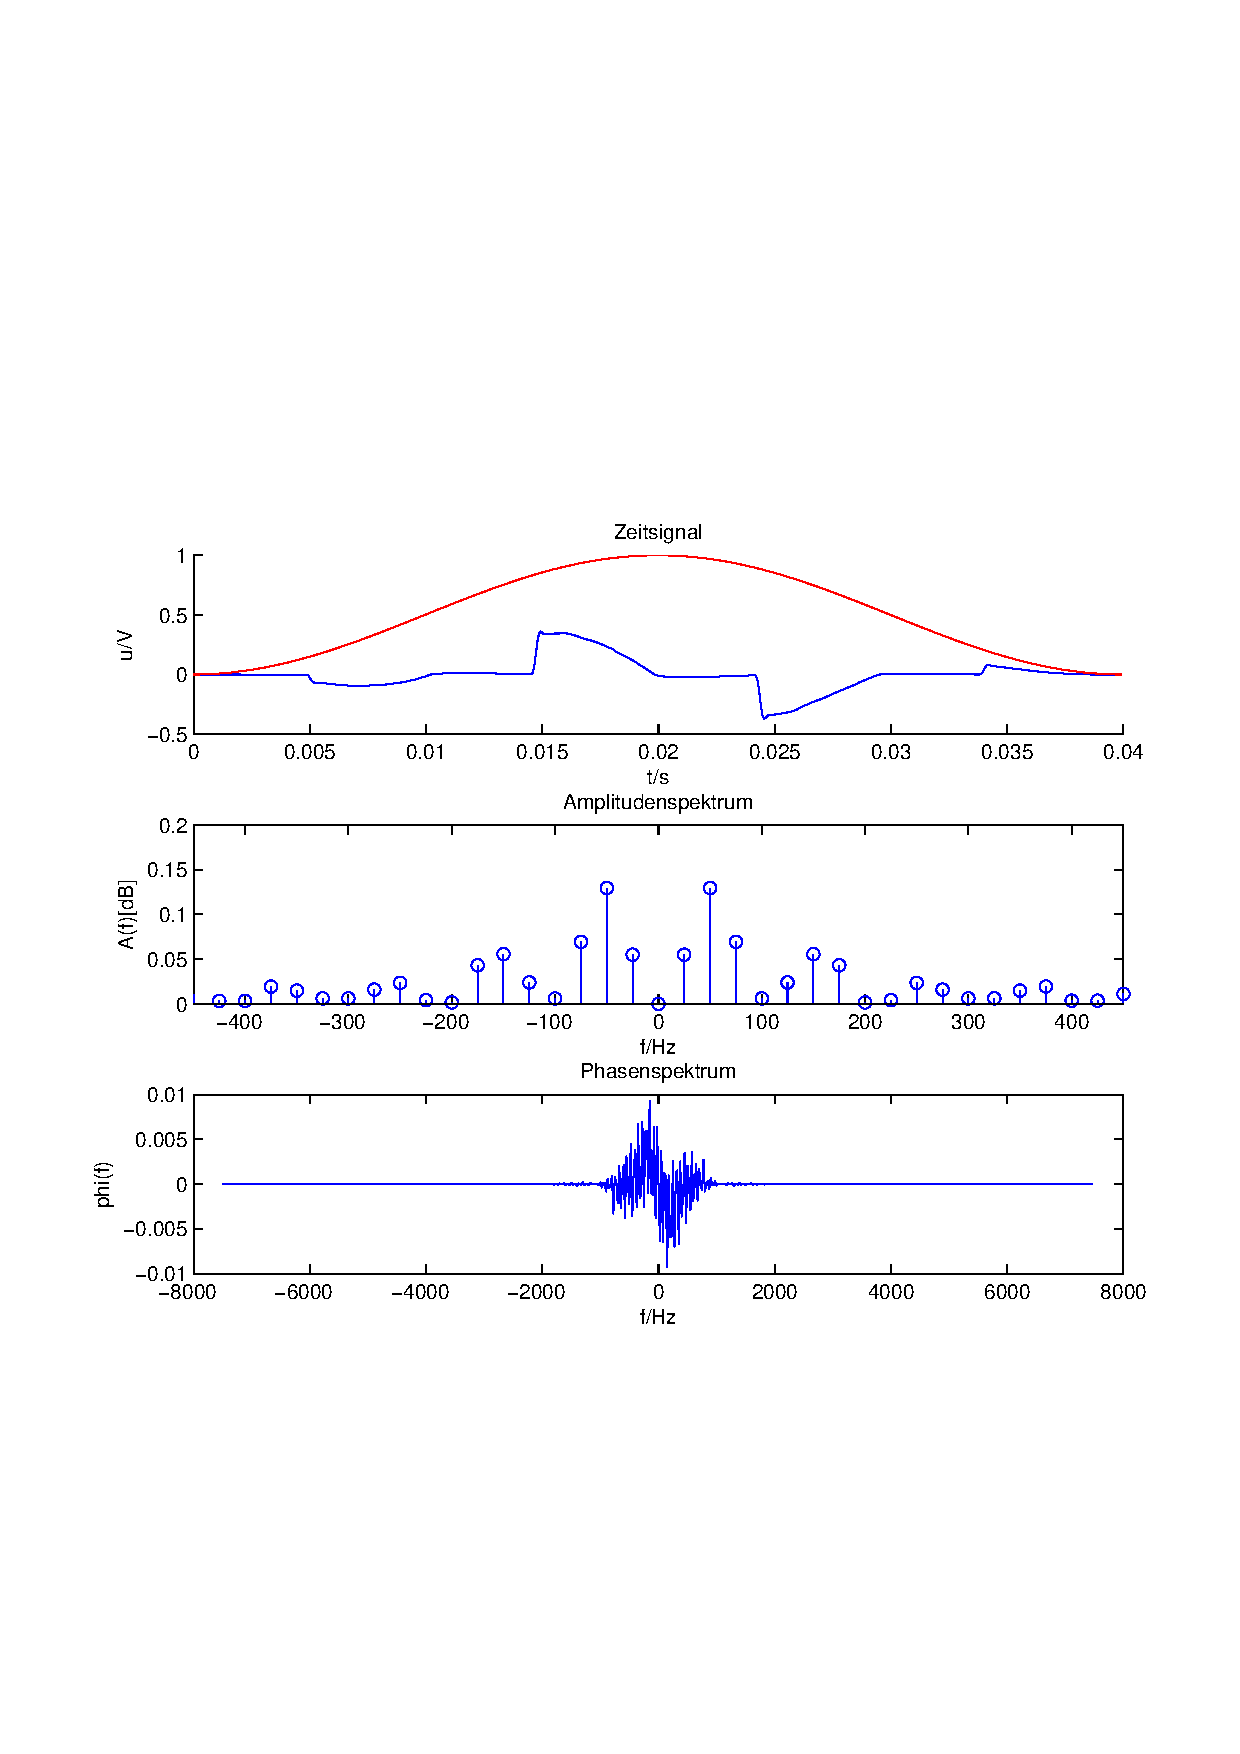
\includegraphics[scale=0.7, trim = 1.5cm 7cm 1.5cm 8.5cm,
                clip]{./Bilder/Phasenanschnittsmessungmithanningfenster.pdf}
                    \caption{Spektrum des angeschnittenen Sinus mit Hanningfenster}
            \end{figure}
    
            Im Vergleich mit der Simulation aus den Vorbereitungsaufgaben von Termin 3, fällt auf, dass die klaren
            Spektrallinien stark verlaufen sind. Der Leckeffekt ist also trotz Fenster aufgetreten. Dies liegt daran,
            dass alle Fensterfunktionen, außer dem Rechteckfenster, das Amplitudenspektrum verlaufen lassen.\\
            Da das Fenster relativ genau 2 Perioden des Messsignals beträgt, kann mit dem Rechteckfenster ein wesendlich
            genaueres Spektrum bestimmt werden.\\
            
            \begin{figure}[H]
            \centering
                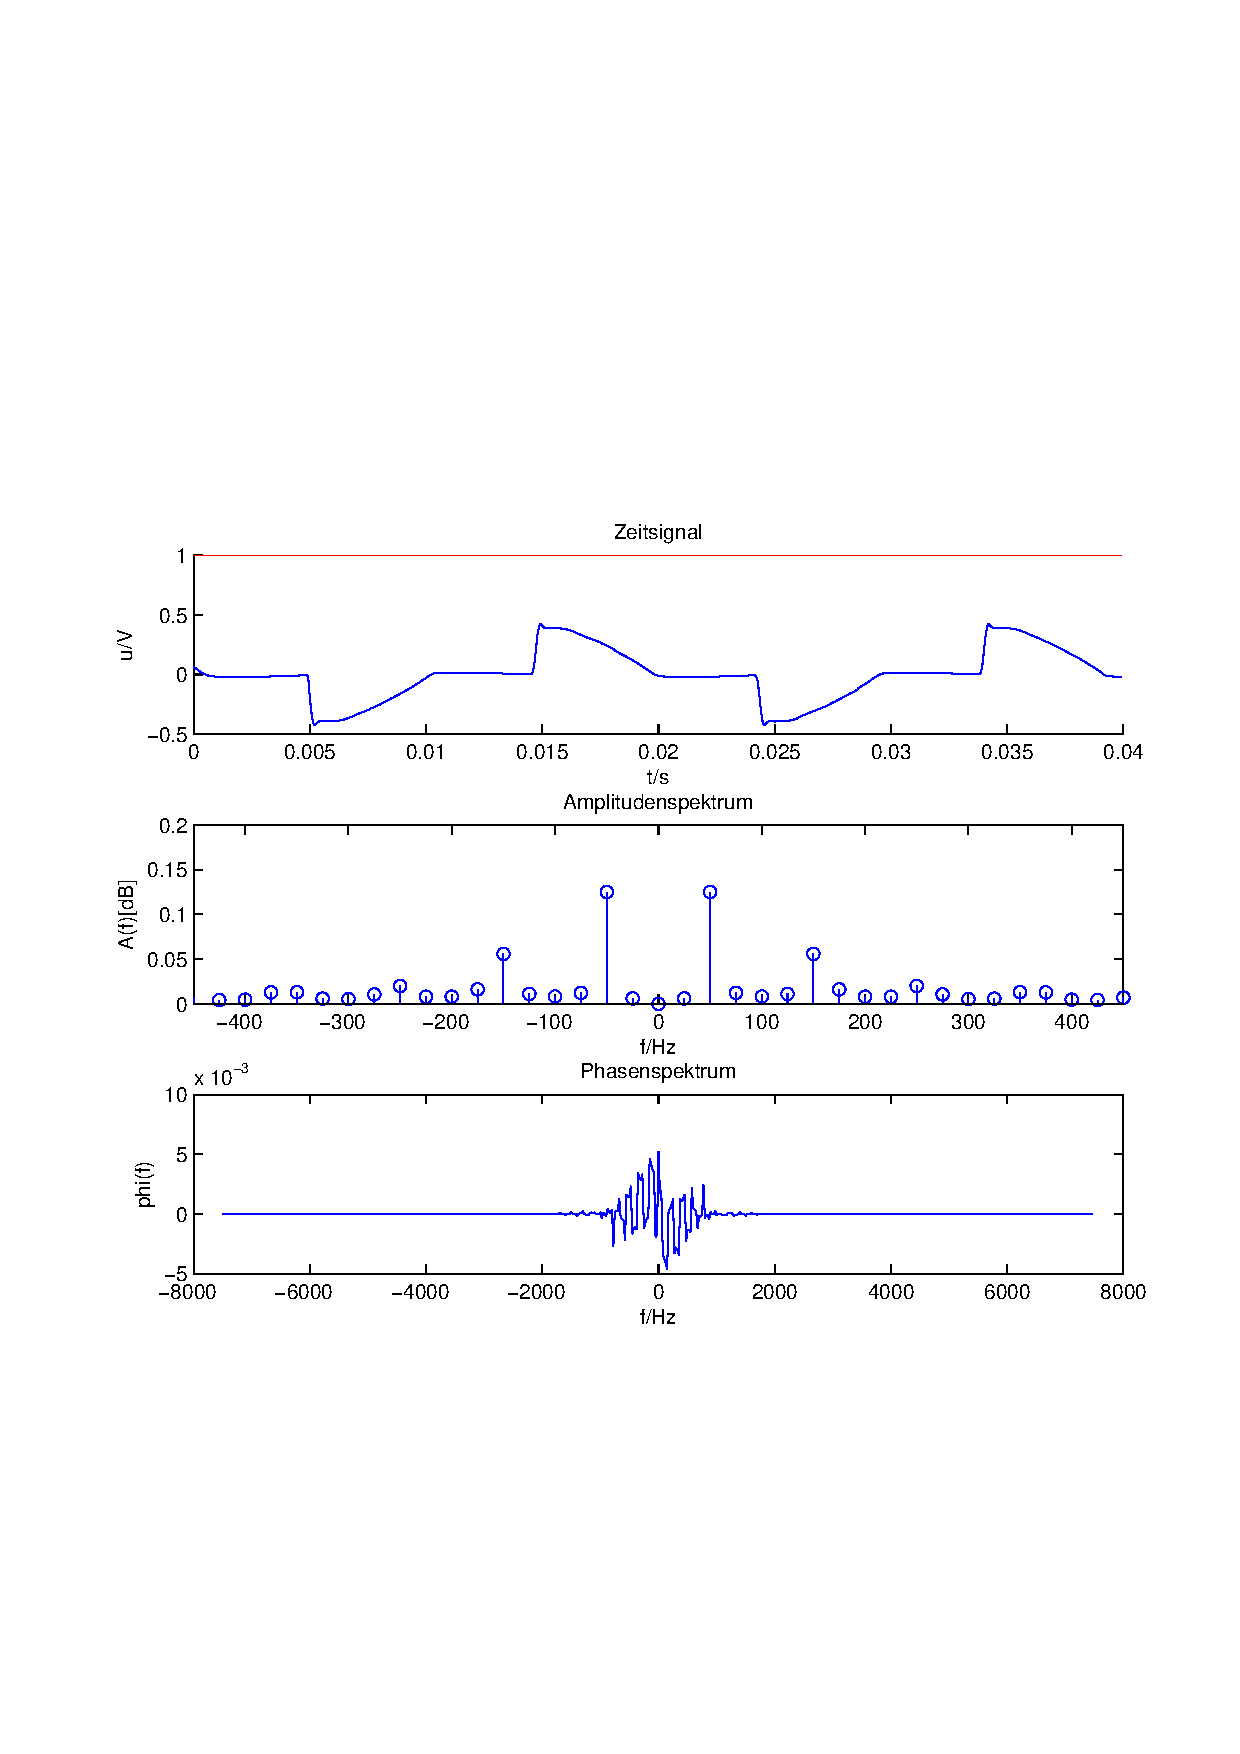
\includegraphics[scale=0.7, trim = 1.5cm 7cm 1.5cm 8.5cm,
                clip]{./Bilder/Phasenanschnittsmessungmitrechteckfenster.pdf}
                    \caption{Spektrum des angeschnittenen Sinus mit Hanningfenster}
            \end{figure}
            
            Wenn das zu messende Signal eine konstante, bekannte Periode besitzt, ist es vorteilhaft ein Rechteckfenster
            zu verwenden. Das Signal kann seine form dabei beliebig verändern. Sollte die Periode des Signals nicht
            konstant sein ist es aber besser eine Fensterfunktion zu verwenden um den Leckeffekt zumindest zu
            verringern.

         \end{quote} % Ende Subsubsection
        
        \subsubsection{Verkürztes Fenster }
<<<<<<< HEAD
		\begin{quote}
			         \begin{figure}[H]
            \centering
                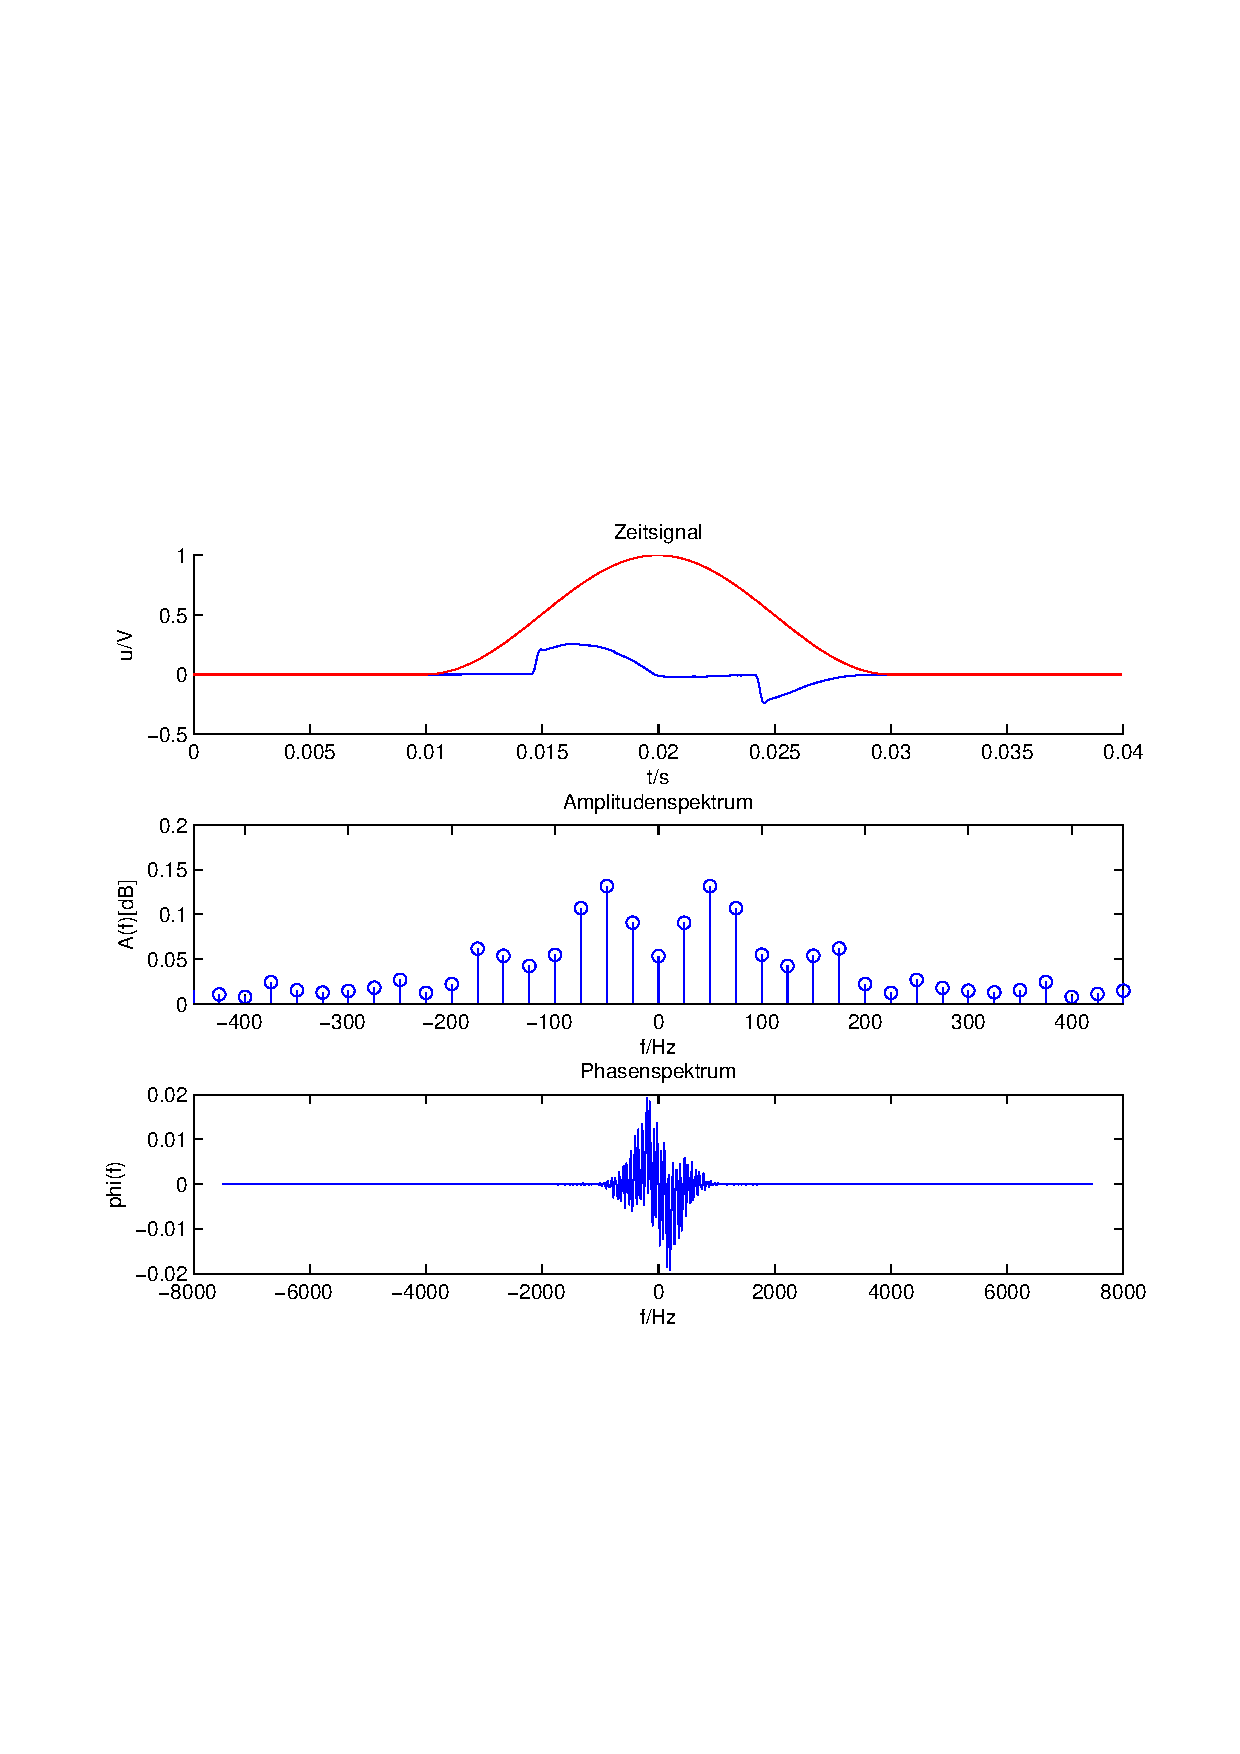
\includegraphics[scale=0.6, trim = 1.5cm 7cm 1.5cm 8.5cm,
                clip]{./Bilder/Phasenanschnittsmessungmithanningfensterleckeffekt}
                    \caption{Phasenanschnittsmessung mit zu kurzem Hanningfenster}
            \end{figure}
        
        \TODO{Boris: Bilder reinhauen wieviele willst du Özgü?}
=======
		\begin{quote}        
                                    %4 Grafiken:
                \begin{center}
                \begin{tabular}{ll}
    
                \hspace{-11em}
                    \begin{minipage}{0.6\textwidth}
    
                        \begin{figure}[H]
                            \label{fig:}
                            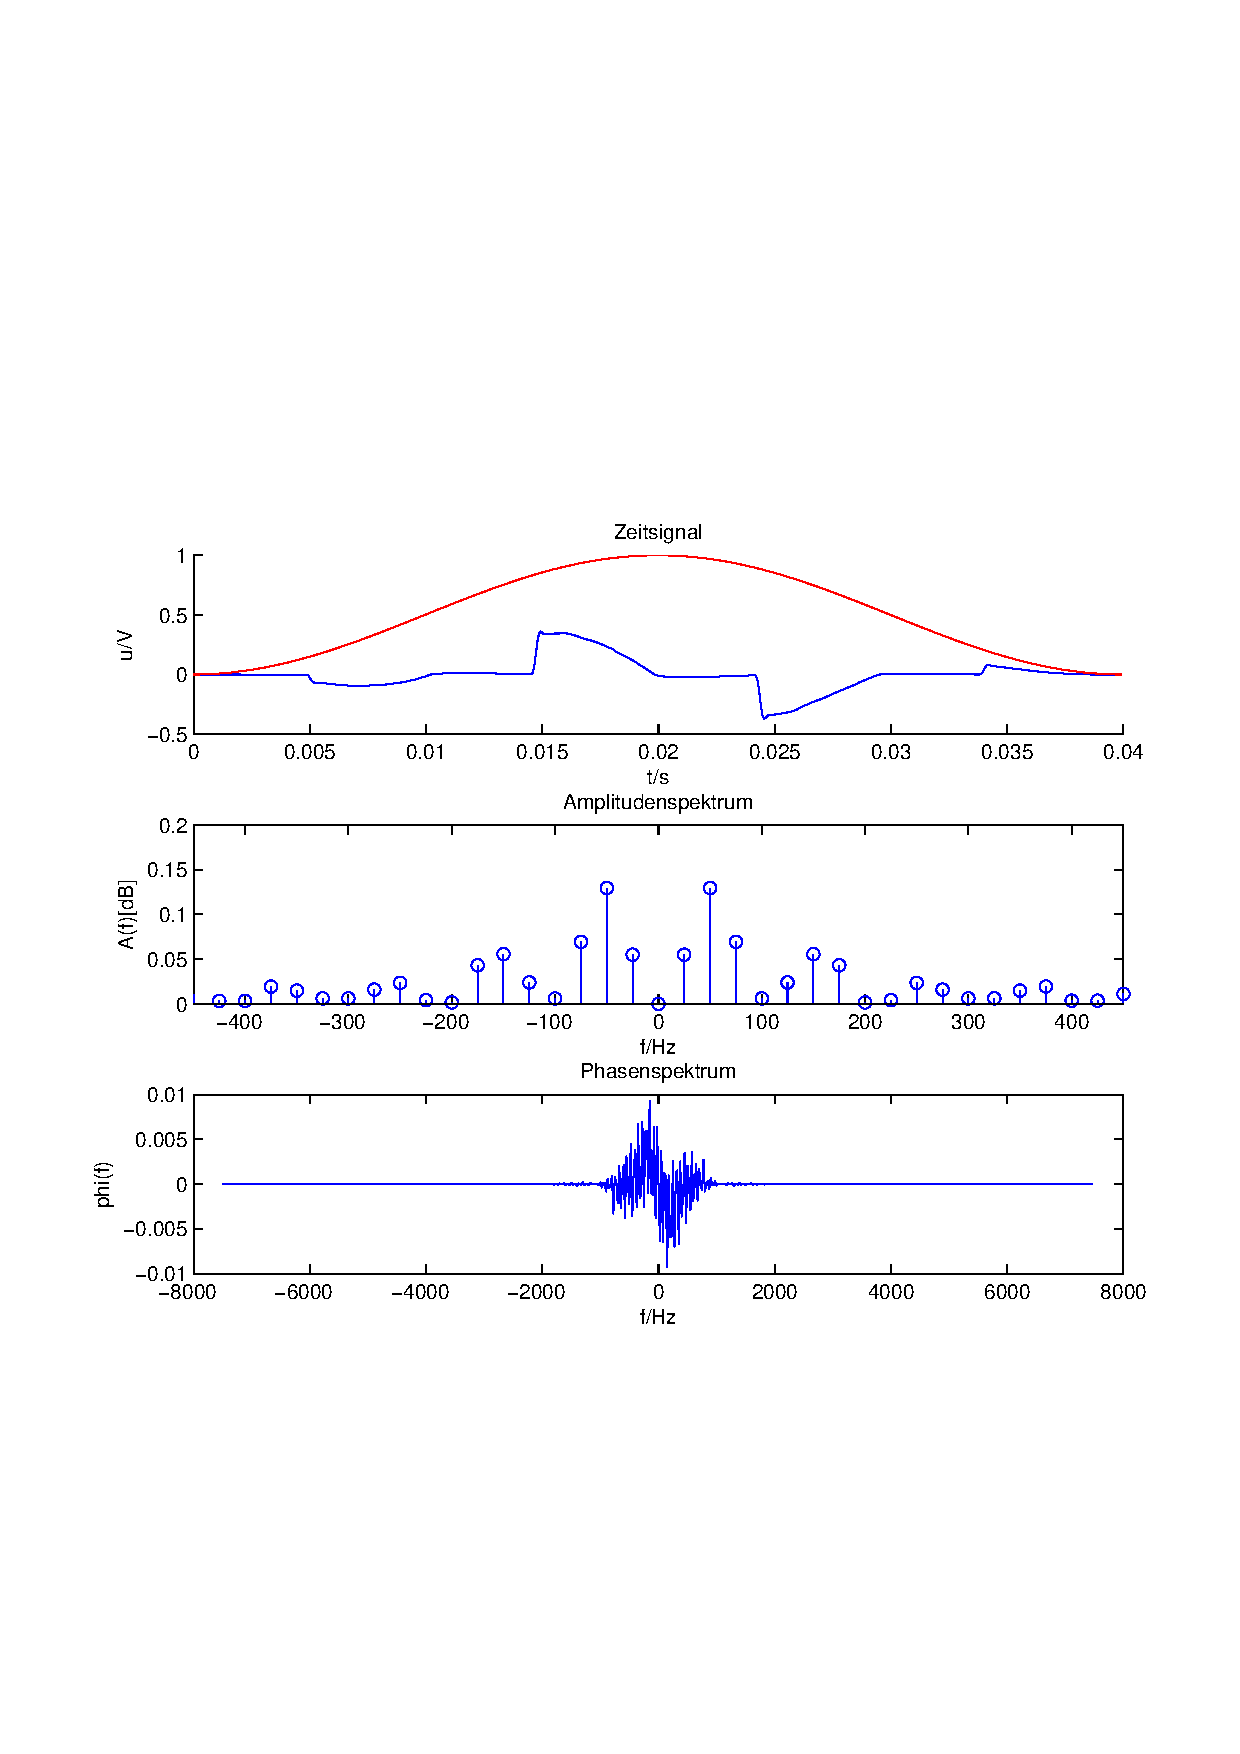
\includegraphics[scale=0.4, trim = 1.5cm 7cm 1.5cm 8cm,
                            clip]{./Bilder/Phasenanschnittsmessungmithanningfenster} %FIXME [width=640px, height=474px]
                            \caption{Phasenanschnittsmessung mit passenden Hanningfenster}
                        \end{figure}
    
                    \end{minipage}
                    \begin{minipage}{0.6\textwidth}
    
                         \begin{figure}[H]
                            \label{fig:}
                            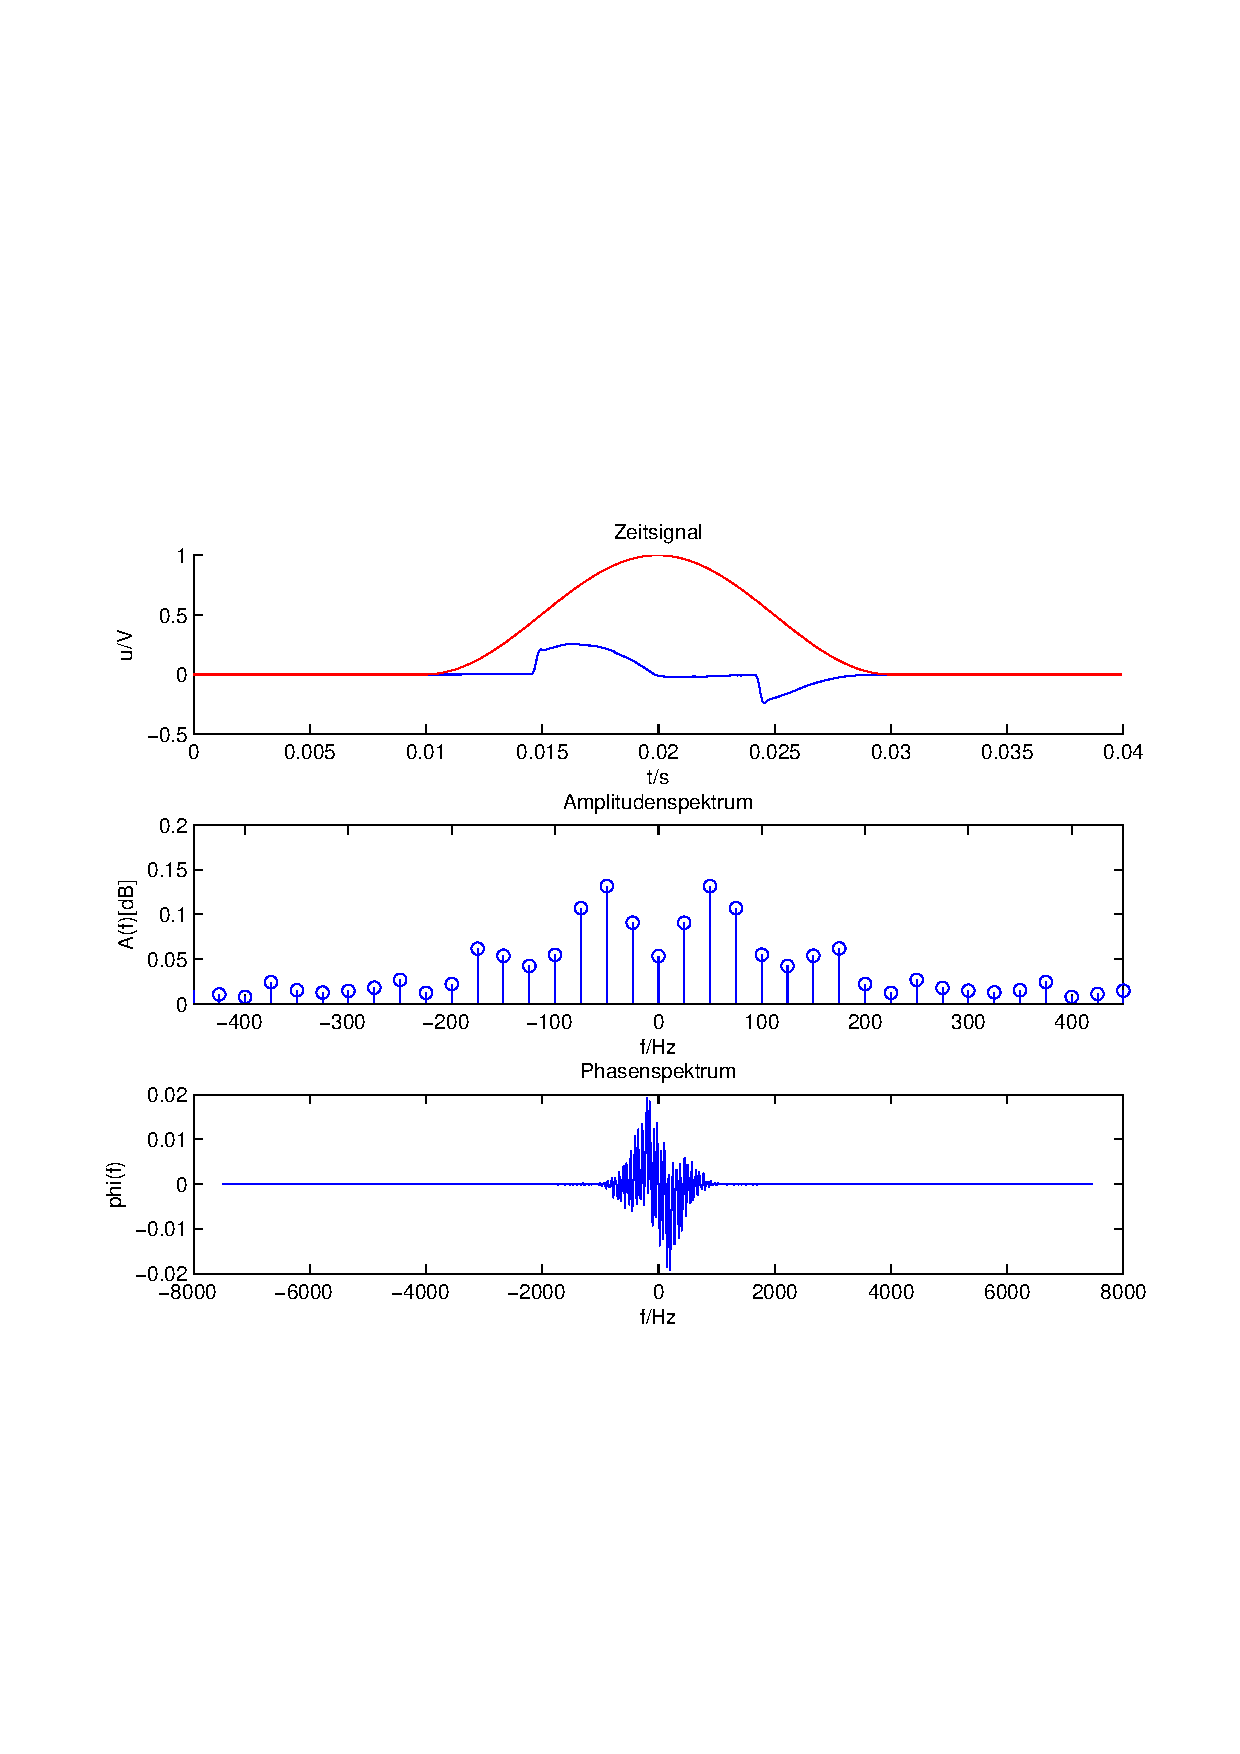
\includegraphics[scale=0.4, trim = 1.5cm 7cm 1.5cm 8cm,
                            clip]{./Bilder/Phasenanschnittsmessungmithanningfensterleckeffekt} %FIXME [width=640px, height=474px]
                            \caption{Phasenanschnittsmessung mit zu kurzem Hanningfenster}
                        \end{figure}
                   \vspace{-1.5em}
    
                    \end{minipage}
    
                \end{tabular}
                \end{center}
                
                \begin{center}
                \begin{tabular}{ll}
    
                \hspace{-11em}
                    \begin{minipage}{0.6\textwidth}
    
                        \begin{figure}[H]
                            \label{fig:}
                            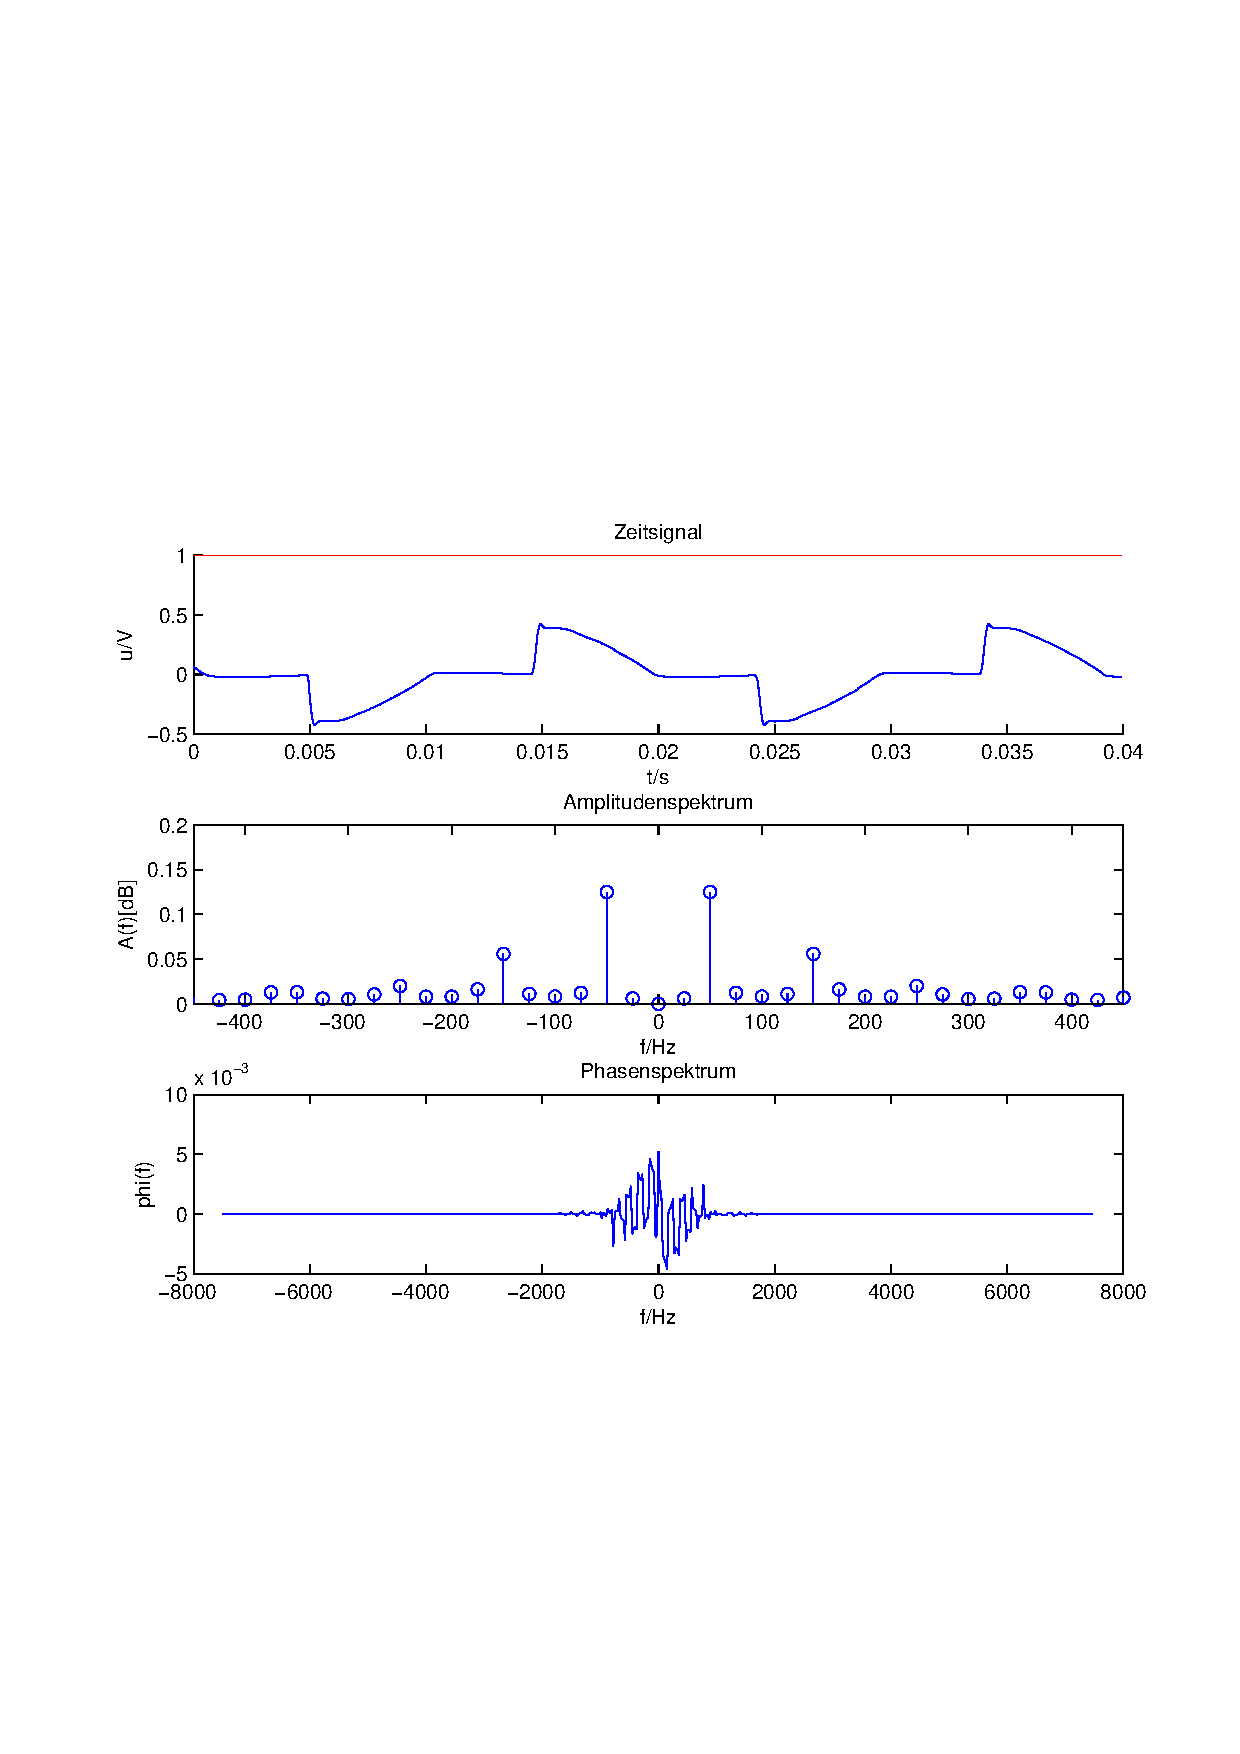
\includegraphics[scale=0.4, trim = 1.5cm 7cm 1.5cm 8cm,
                            clip]{./Bilder/Phasenanschnittsmessungmitrechteckfenster} %FIXME [width=640px, height=474px]
                            \caption{Phasenanschnittsmessung mit passenden Rechteckfenster}
                        \end{figure}
    
                    \end{minipage}
                    \begin{minipage}{0.6\textwidth}
    
                         \begin{figure}[H]
                            \label{fig:}
                            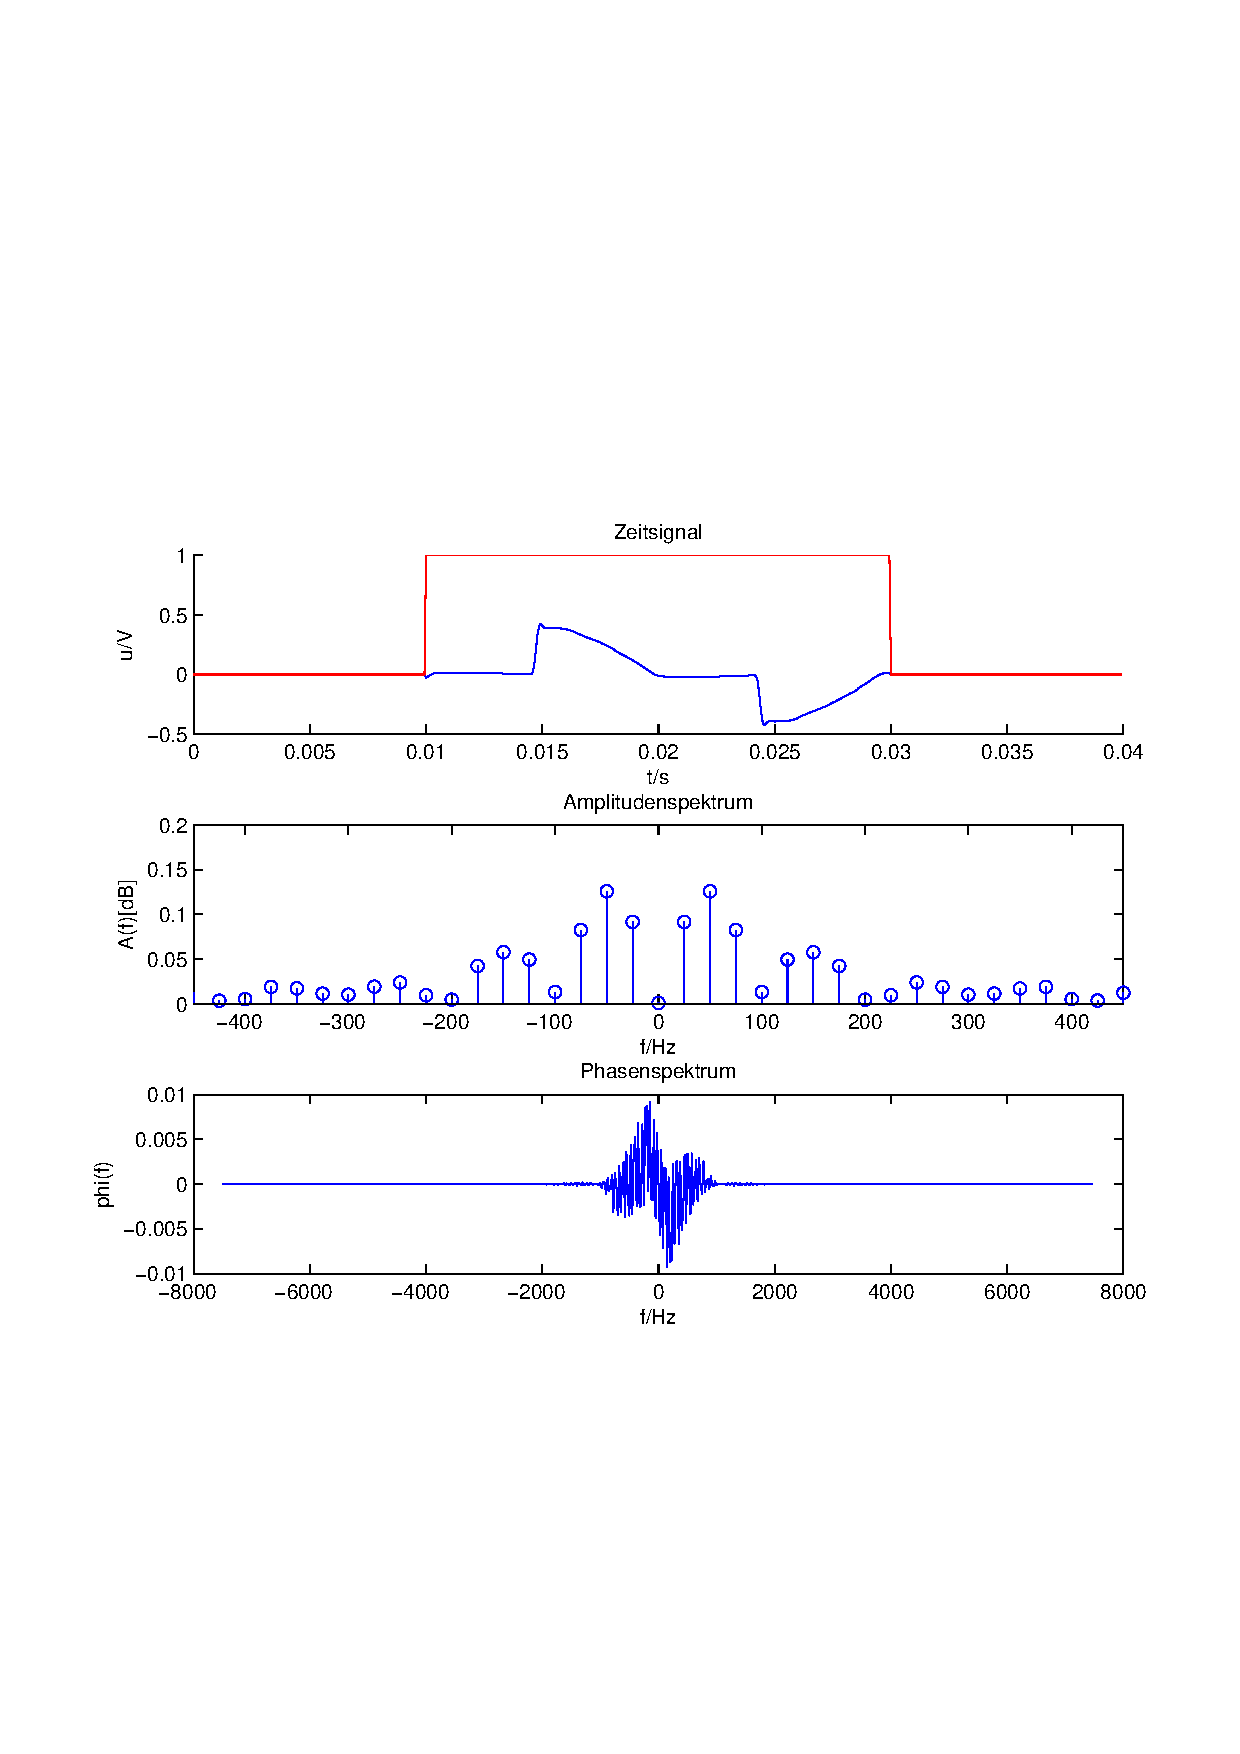
\includegraphics[scale=0.4, trim = 1.5cm 7cm 1.5cm 8cm,
                            clip]{./Bilder/Phasenanschnittsmessungmitrechteckfensterleckeffekt} %FIXME [width=640px, height=474px]
                            \caption{Phasenanschnittsmessung mit zu kurzem Rechteckfenster}
                        \end{figure}
                   \vspace{-1.5em}
    
                    \end{minipage}
    
                \end{tabular}
                \end{center}                
        
                \begin{center}
                \begin{tabular}{ll}
    
                \hspace{-11em}
                    \begin{minipage}{0.6\textwidth}
    
                        \begin{figure}[H]
                            \label{fig:}
                            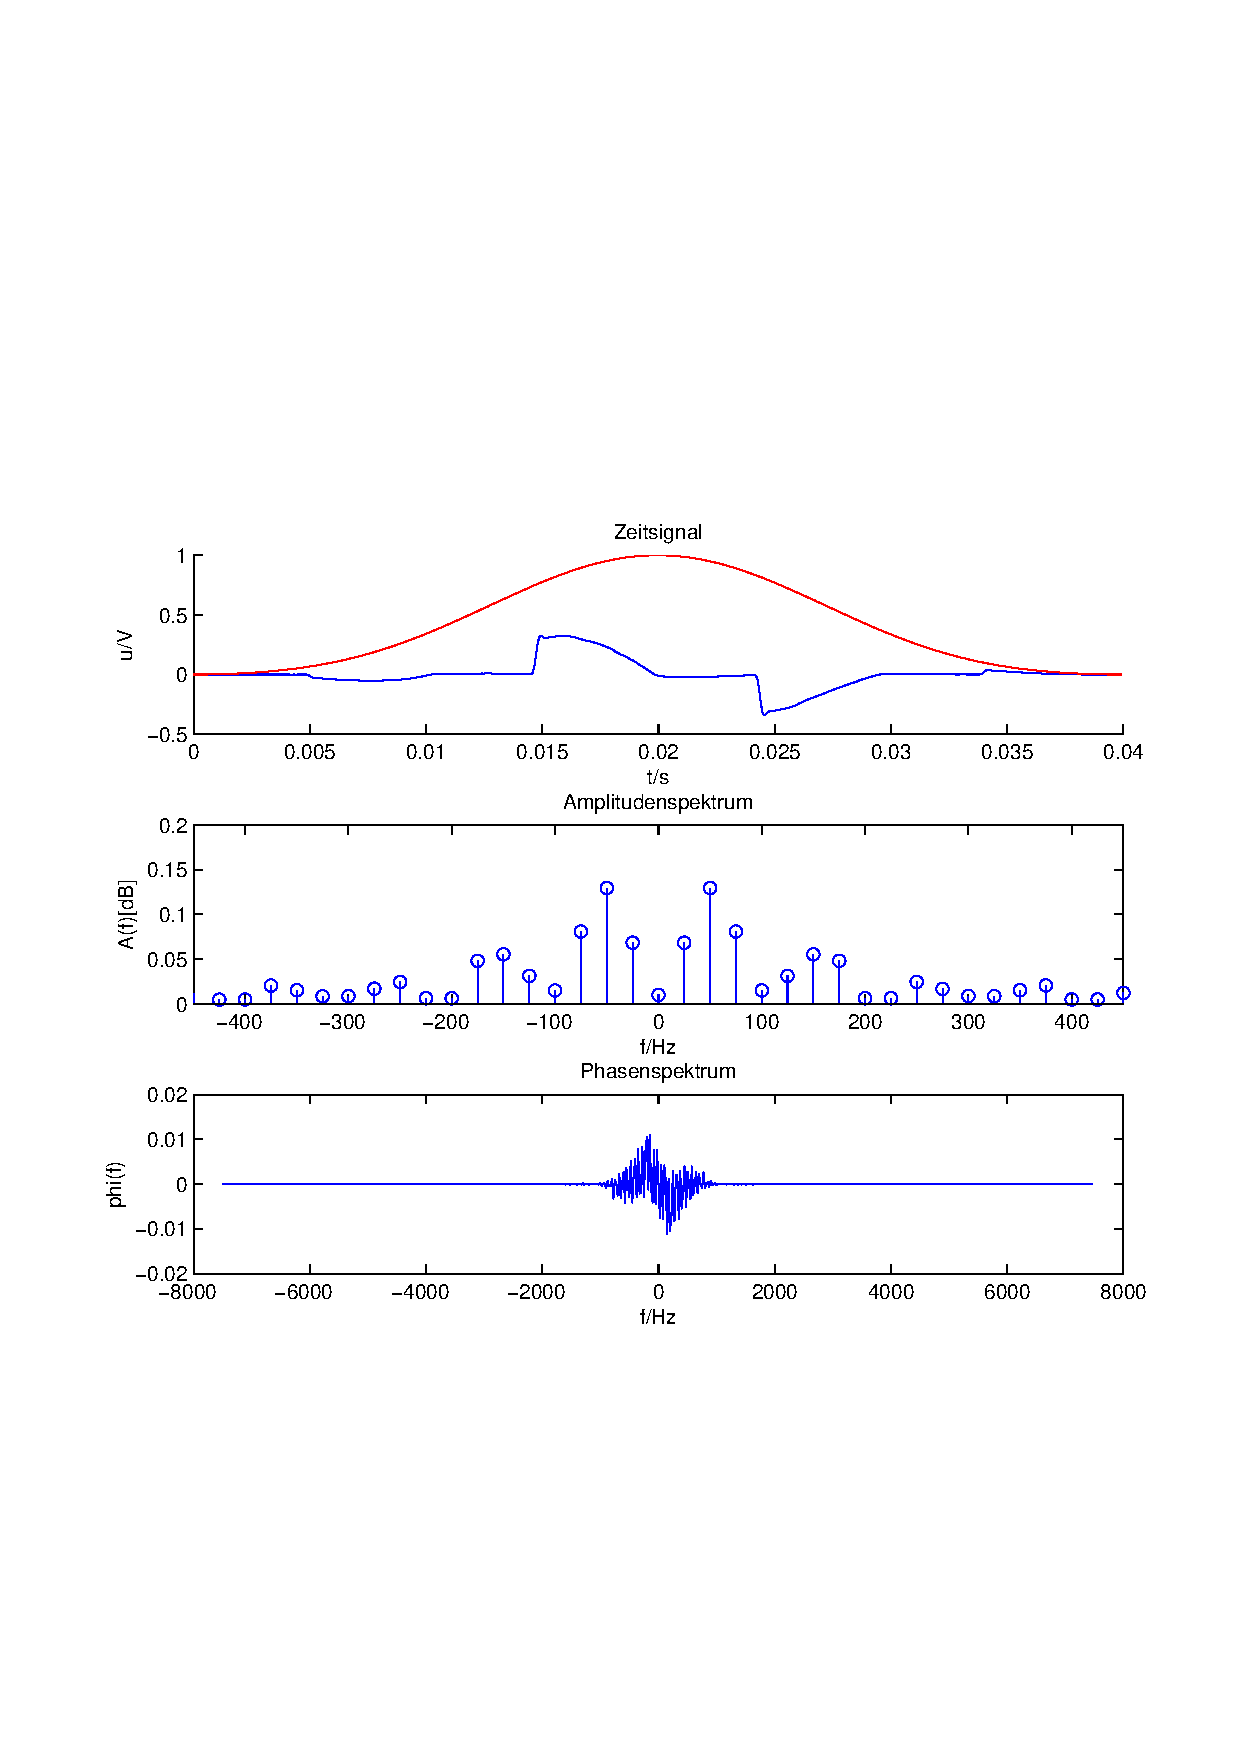
\includegraphics[scale=0.4, trim = 1.5cm 7cm 1.5cm 8cm,
                            clip]{./Bilder/Phasenanschnittsmessungmitblackmanfenster} %FIXME [width=640px, height=474px]
                            \caption{Phasenanschnittsmessung mit passenden Blackmanfenster}
                        \end{figure}
    
                    \end{minipage}
                    \begin{minipage}{0.6\textwidth}
    
                         \begin{figure}[H]
                            \label{fig:}
                            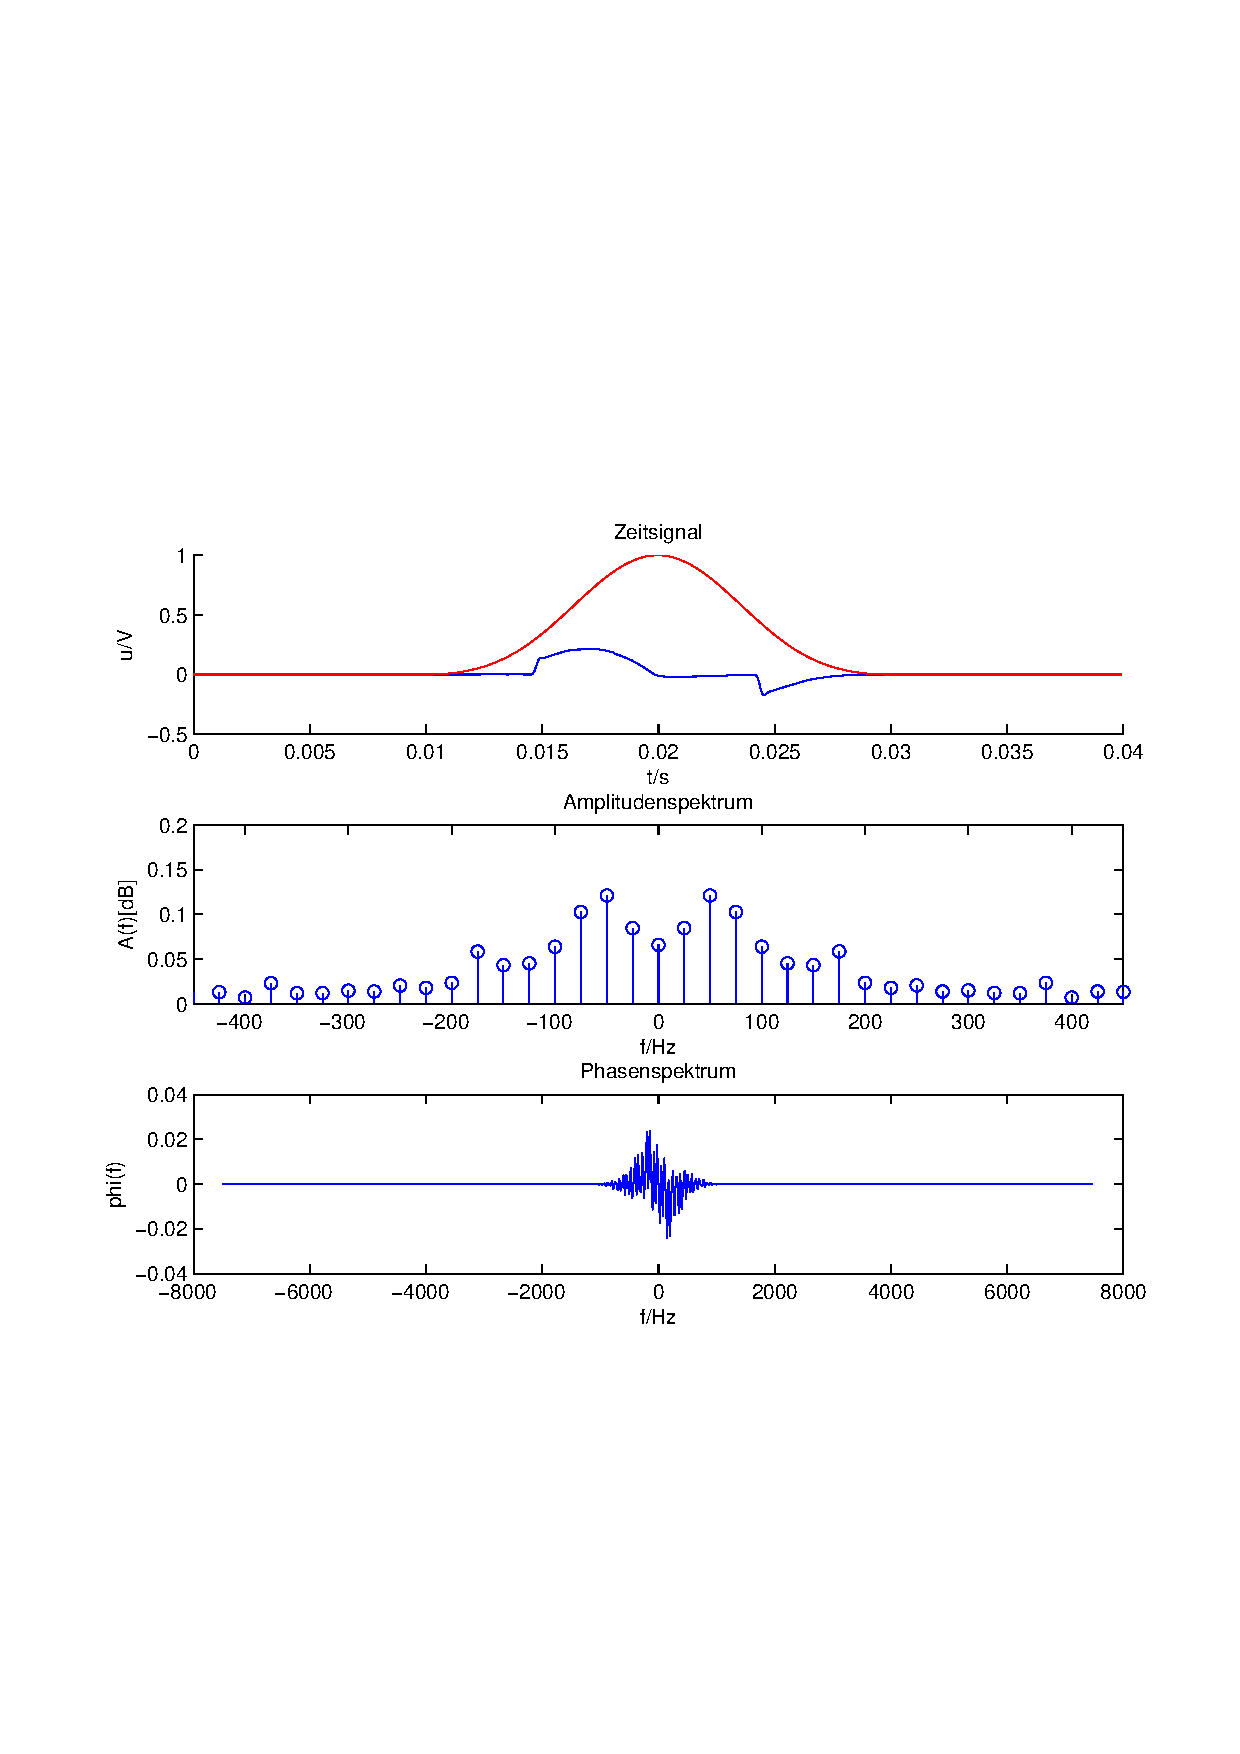
\includegraphics[scale=0.4, trim = 1.5cm 7cm 1.5cm 8cm,
                            clip]{./Bilder/Phasenanschnittsmessungmitblackmanfensterleckeffekt} %FIXME [width=640px, height=474px]
                            \caption{Phasenanschnittsmessung mit zu kurzem Blackmanfenster}
                        \end{figure}
                   \vspace{-1.5em}
    
                    \end{minipage}
    
                \end{tabular}
                \end{center}
                \vspace{1em}
>>>>>>> branch 'master' of git@github.com:unizeug/Messdatenverarbeitung_OETB_Termin3.git
        
        Diese Simmulation zeigt die Auswirkungen bei Entstehung des
        Leck-Effekts bei einem zu kurz gewählten Hanningfenster. Als Ergebnis ist ein
        etwas breiteres und flacheres Spektrum zu sehen, wie es zu erwarten war.
		\end{quote} % Ende Subsubsection
         
        \subsubsection{Netzqualität bestimmen}
    	\begin{quote}
    		Die Qualität der Netzspannung wird mit folgender Formel bestimmt.
    		
    		\begin{align}
                THD = \frac{\sqrt{{U_2}^2+{U_3}^2+ \cdot + {U_N}^2}}{U_1}
            \end{align}
            
            Es wird die geometrische Summe aller Oberwellen gebildet und durch die Grundwelle geteilt.
            Dabei ergab sich ein Anteil der Oberwellen von $3,32\%$ an dem gesamten Signal. Dieser Wert liegt unter den
            maximal zulässigen $8\%$.\\
            Es ist zu beachten, das nicht alle Oberwellen gemessen wurden und dadurch auch nicht berücksichtigt wurden.
            Durch den Antiallaisingfilter wurden alle Frequenzen oberhalb von 7kHz ausgesperrt. Schnelle Störnadeln, die
            durch Schaltvorgänge entstehen und in einem Stromversorgungsnetz häufig vorkommen, werden daher nicht
            vollständig berücksichtigt. Daher wird THD tatsächlich etwas höher sein als der hier ermittelte Wert.
            
            \begin{figure}[H]
            \centering
                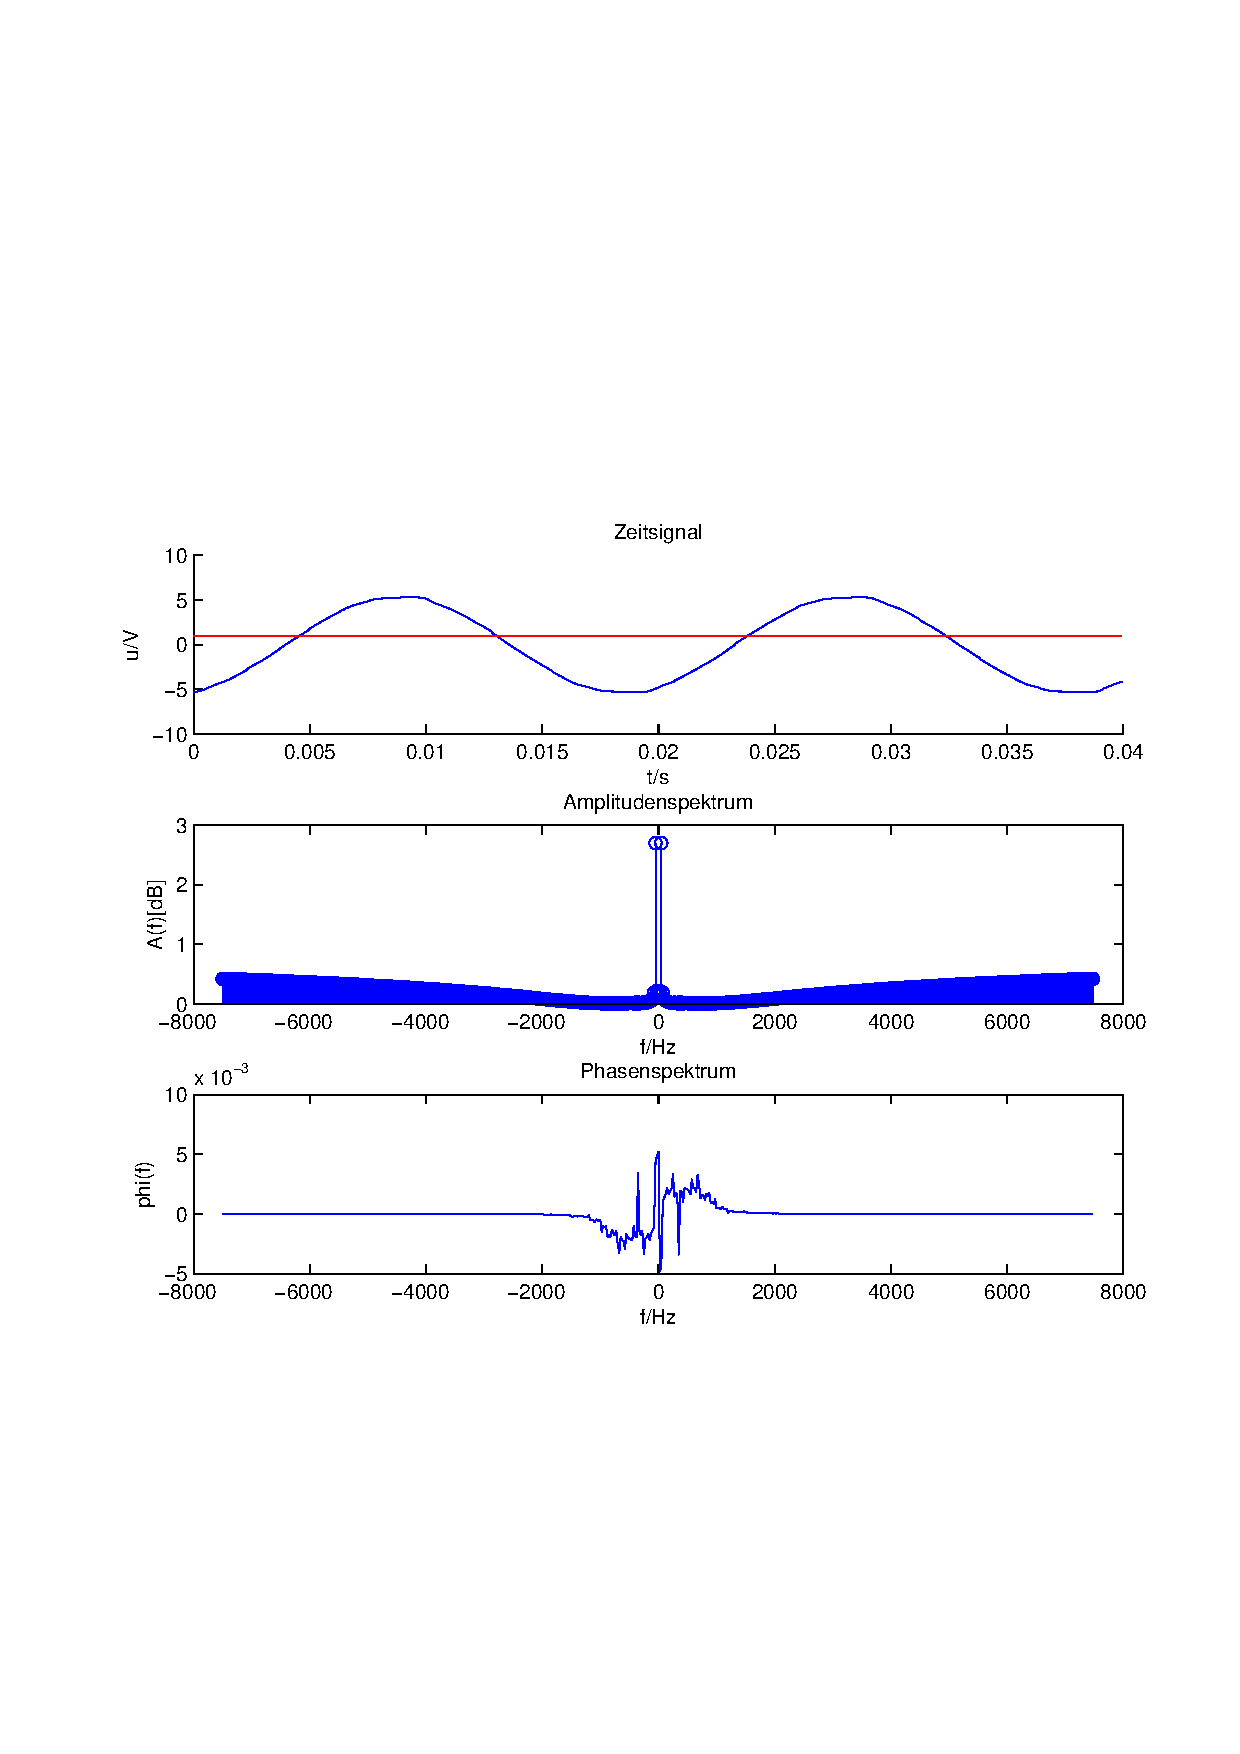
\includegraphics[scale=0.7, trim = 1.5cm 7cm 1.5cm 8.5cm, clip]{./Bilder/OberwellenmessungspektrumTHD00332.pdf}
                    \caption{caption}
            \end{figure}
    

    	\end{quote} % Ende Subsubsection
    
    \end{quote}  % Ende Subsection
			
\end{quote}%Ende section
%--------------------------------------------------------------------
%--------------------------------------------------------------------
\section{Quellcodes}
\begin{quote}
	
	\subsection{Codes aus Termin 3}
	\begin{quote}
	    \subsubsection{sinus2.m}
	    \begin{quote}
	        \lstinputlisting[
	            caption={sinus2},
	            label=lst:Matlab]
	            {./Matlab/sinus2.m}
	    \end{quote}
    
	    \subsubsection{stromPhasSchnitt.m}
	    \begin{quote}
	        \lstinputlisting[
	            caption={stromPhasSchnitt},
	            label=lst:Matlab]
	            {./Matlab/stromPhasSchnitt.m}
	    \end{quote}
    
	    \subsubsection{EffektivwertZeitbereich.m}
	    \begin{quote}
	        \lstinputlisting[
	            caption={EffektivwertZeitbereich},
	            label=lst:Matlab]
	            {./Matlab/EffektivwertZeitbereich.m}
	    \end{quote}
    
	    \subsubsection{EffektivwertFourier.m}
	    \begin{quote}
	        \lstinputlisting[
	            caption={EffektivwertFourier},
	            label=lst:Matlab]
	            {./Matlab/EffektivwertFourier.m}
	    \end{quote}
	    \subsubsection{alphadetektor2.m}
        \begin{quote}
            \lstinputlisting[
                caption={alphadetektor2},
                label=lst:Matlab]
                {./Matlab/alphadetektor2.m}
        \end{quote}
        
        \subsubsection{Aufgabe33.m}
        \begin{quote}
            \lstinputlisting[
                caption={Aufgabe33},
                label=lst:Matlab]
                {./Matlab/Aufgabe33.m}
        \end{quote}
        
        \subsubsection{Spektrum2Filterkorrektur.m}
        \begin{quote}
            \lstinputlisting[
                caption={Spektrum2Filterkorrektur},
                label=lst:Matlab]
                {./Matlab/Spektrum2Filterkorrektur.m}
        \end{quote}
	\end{quote}
	
	\subsection{Codes aus Termin 4}
	\begin{quote}
		
		\subsubsection{Spektrum.m}
		\begin{quote}
		\lstinputlisting[
				caption={Spektrum},
				label=lst:Matlab]
				{./Matlab/Spektrum.m}
		\end{quote}
		
		\subsubsection{Spektrum2Filterkorrektur.m}
        \begin{quote}
        \lstinputlisting[
                caption={Spektrum2Filterkorrektur},
                label=lst:Matlab]
                {./Matlab/Spektrum2Filterkorrektur.m}
        \end{quote}
		
		\subsubsection{Vorbereitungsaufgabe2.m}
		\begin{quote}
		\lstinputlisting[
				caption={},
				label=lst:Matlab]
		        {./Matlab/Vorbereitungsaufgabe42.m}
		\end{quote}
		
		\subsubsection{Vorbereitungsaufgabe3.m}
		\begin{quote}
		\lstinputlisting[
				caption={Vorbereitungsaufgabe43},
				label=lst:Matlab]
                {./Matlab/Vorbereitungsaufgabe43.m}		
		\end{quote}
		
		\subsubsection{praxisaufgabe41.m}
        \begin{quote}
        \lstinputlisting[
                caption={praxisaufgabe41},
                label=lst:Matlab]
                {./Matlab/praxisaufgabe41.m}     
        \end{quote}
        
        \subsubsection{MDV PR4 aufgabe3.m}
        \begin{quote}
        \lstinputlisting[
                caption={MDV PR4 aufgabe3},
                label=lst:Matlab]
                {./Matlab/MDV_PR4_aufgabe3.m}     
        \end{quote}
		
	\end{quote}
\end{quote}



%--------------------------------------------------------------------
%--------------------------------------------------------------------


\begin{thebibliography}{999}
\bibitem {Schaltungwandlerbox} Prof. Dr.-Ing. Gühmann, Clemens; Dipl.-Ing. Funk, Jürgen: MDVLaborGeraete_web, S.4

%Name, Vorname.; evtl. Name2, Vorname2.: Titel des Dokumentes
%oder Buches, Zeitschrift/Verlag/URL (Auflage, Erscheinungsort, -jahr), ggf. Seitenzahlen
\bibitem {PasevalscheTheorem} \url{https://de.wikipedia.org/wiki/Parsevalsches_Theorem}, Zugriff
23.05.2012
\end{thebibliography}


\end{document}


